\section{Reweight Dedicated TT MC Samples for the Estimation of theoretical uncertainties}

The size of the uncertainty resulting from the FSR variation is observed
to be very large (up to 20\%) in the $\ell\tau$ categories.  This level
of variation could be expected to be corrected for in the scale factors
accounting for the difference in ID/misID efficiency for identified
$\tau$ candidates, and that uncertainty in general would be much
smaller, $<5\%$.  

To account for this, scale factors between the different
simulation scenarios are estimated.  Since these are corrections
between MC, the scale factors are derived using generator truth
information.  That is, while running over the nominal and FSR-scaled
$\ttbar$ samples, $W\rightarrow\tau_{h}$ are identified.  The efficiency
of these generator level, hadronic taus to be matched to a reconstructed
$\tau_{h}$ passing all identification requirements is evaluated.  Based
on this scale factors between the up and down variations can be
calculated.  The resulting values are shown in figure~\ref{fig:appendix:reweighttt:sf_fsr}.
Based on this, the morphing templates in the $\ell\tau$ categories are
scaled according to the average scale factor for the
$\tau\rightarrow\tau$ and $j \rightarrow \tau$ templates. The effect of
including the corrections for the FSR-varied samples is shown in
table~\ref{tab:fsr_correction}.  It is clear that there is a substantial
reduction in the uncertainty attributable to the FSR variations.



\begin{table}[h]
    \begin{center}
    \begin{tabular}{l|cccc}
                                  & $W\rightarrow e$ & $W\rightarrow \mu$ & $W\rightarrow \tau$ & $W\rightarrow h$ \\
        \hline
        nominal                   & 1.02             & 0.71               & 2.04                & 0.40             \\
        w/ $\tau$ FSR corrections & 1.01             & 0.69               & 1.69                & 0.36             \\
    \end{tabular}
    \caption{Comparison between nominal uncertainty (in a snapshot of
        the analysis) and the uncertainty after applying the corrections
        to the FSR variation.}
    \label{fig:fsr_correction}
    \end{center}
\end{table}



\begin{figure}
    \centering
    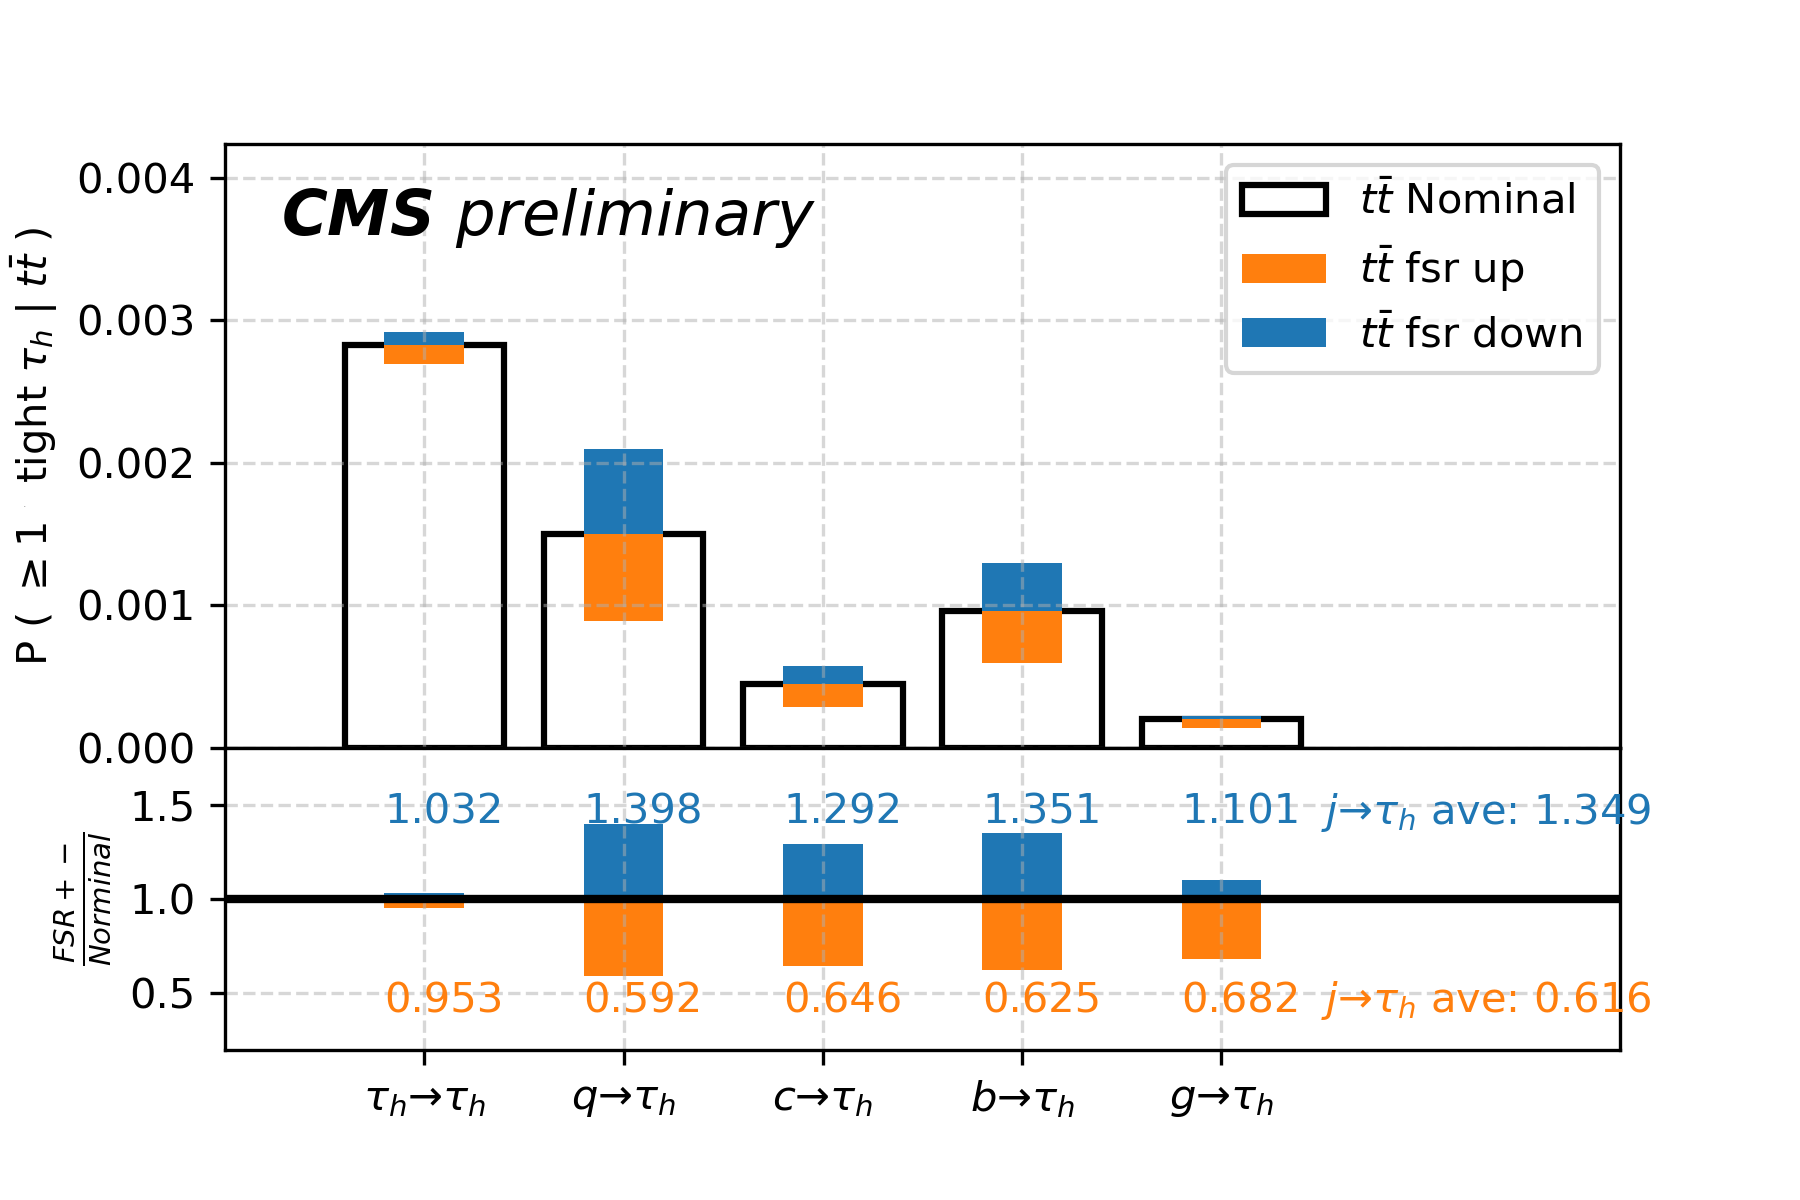
\includegraphics[width=0.49\textwidth]{chapters/Appendix/sectionTTSyst/figures/2020_MCRatio_fsr_tauGenFlavor_tauTight.png}
    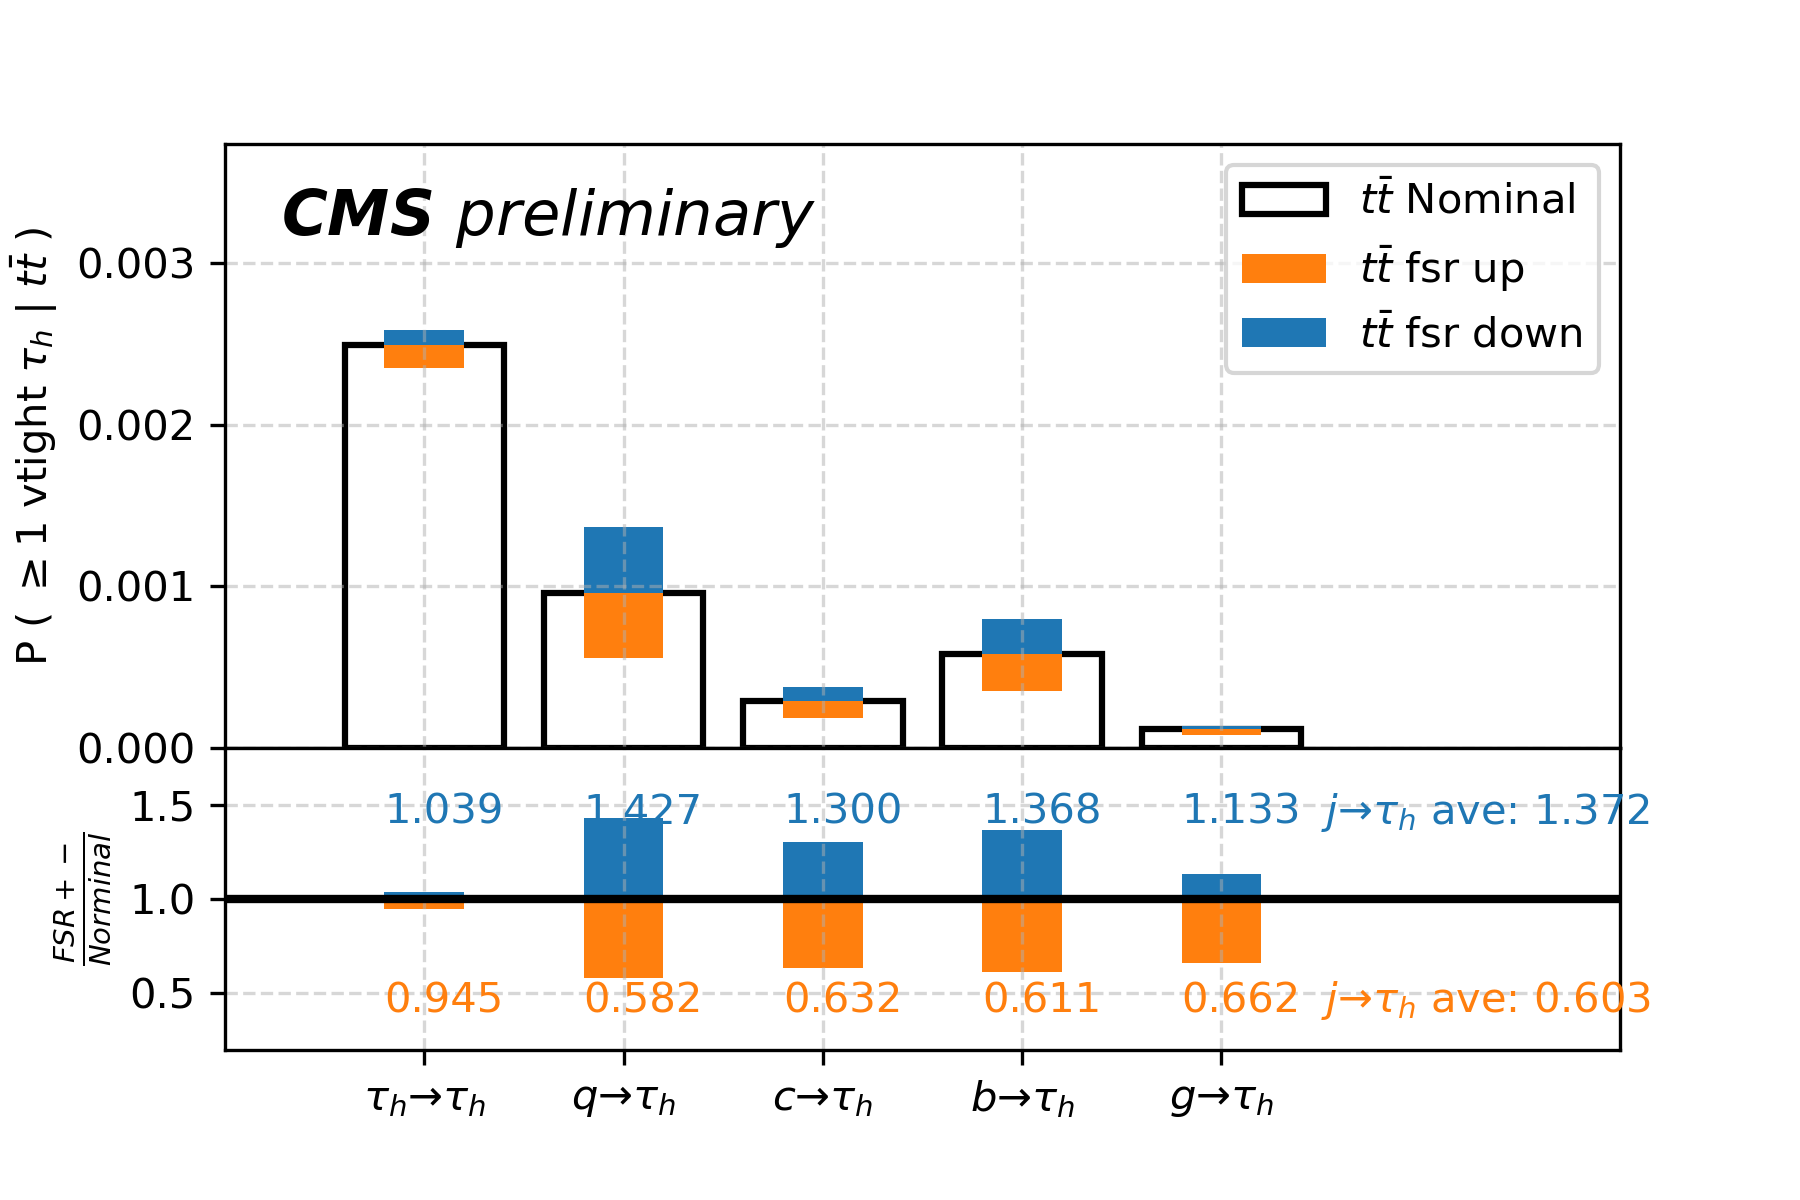
\includegraphics[width=0.49\textwidth]{chapters/Appendix/sectionTTSyst/figures/2020_MCRatio_fsr_tauGenFlavor_tauVTight.png}
    \caption{Reweight $\tau_h$ and $j \to \tau_h$ efficiencies in the dedicated FSR ttbar samples}
    \label{fig:appendix:reweighttt:sf_fsr}
\end{figure}

\begin{figure}
    \centering
    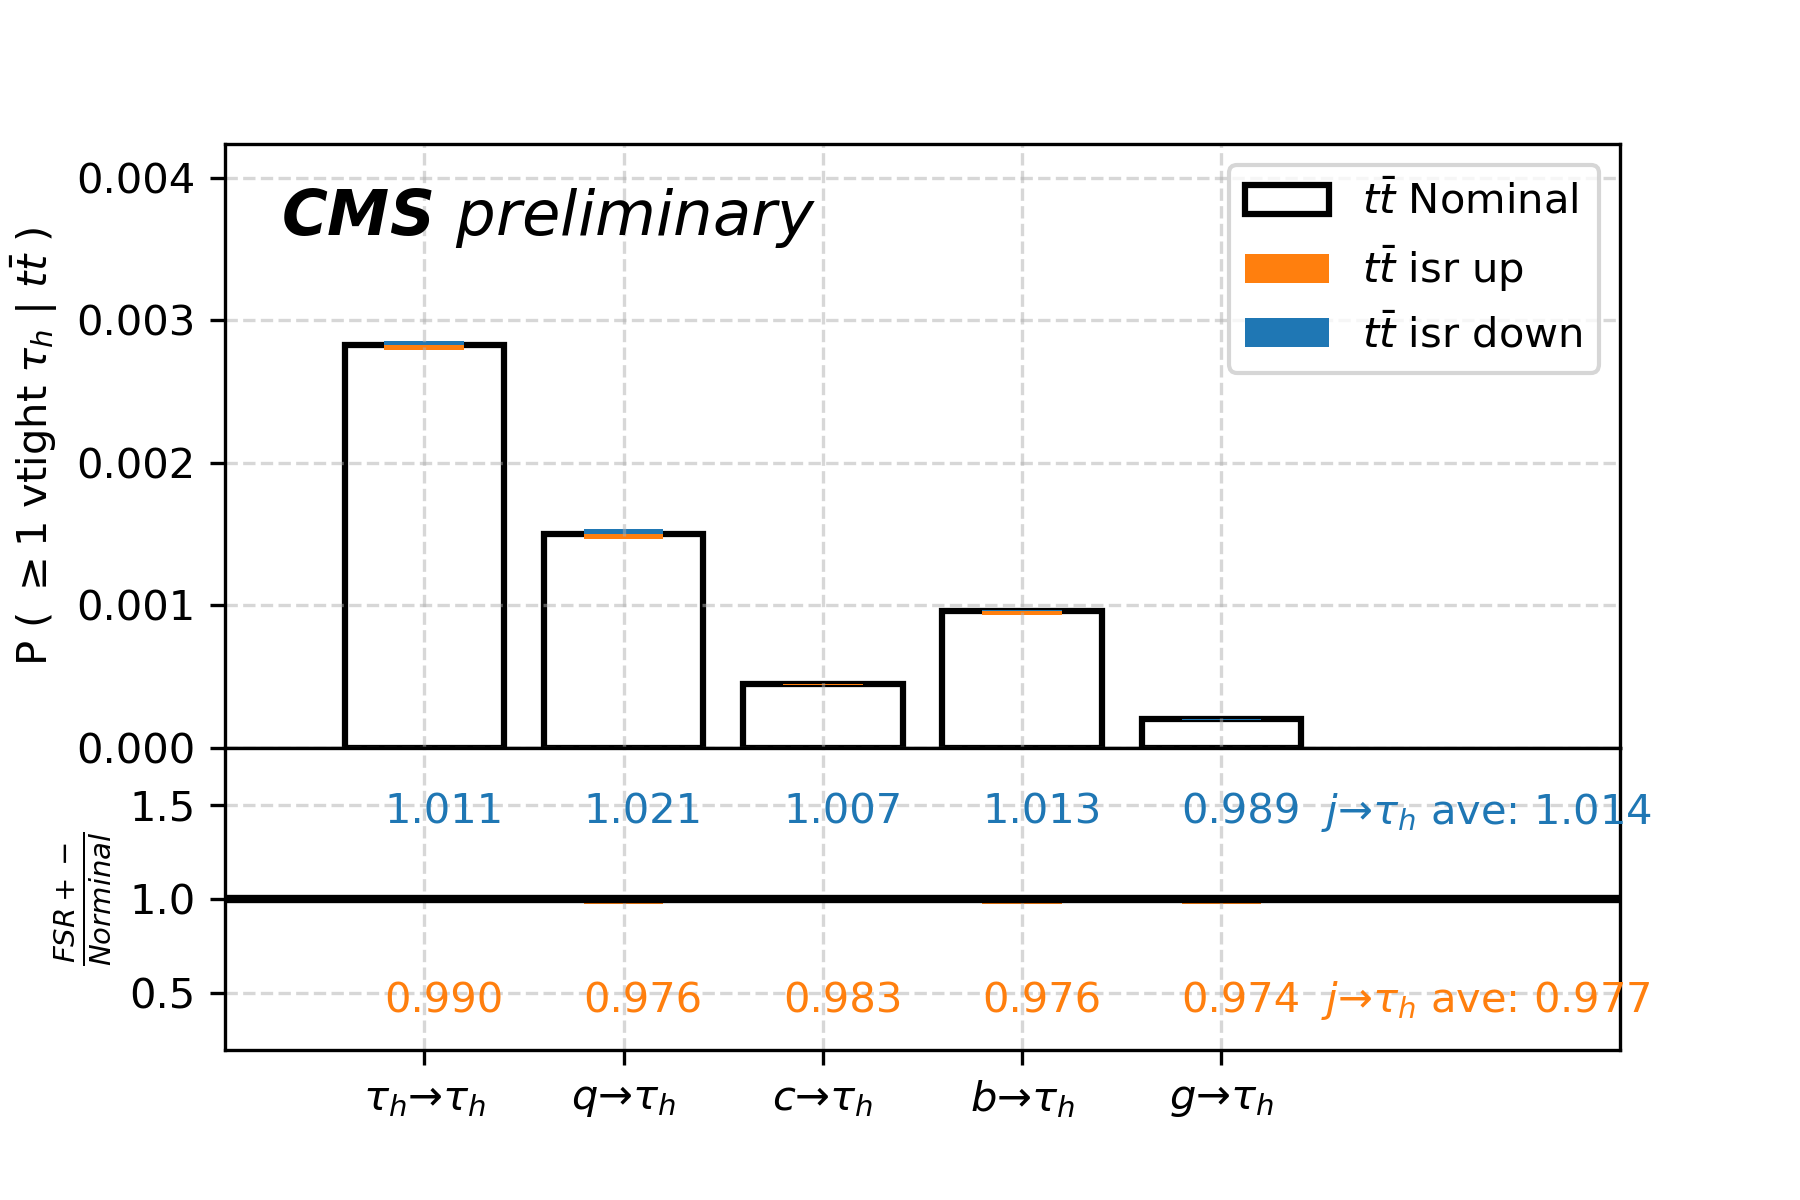
\includegraphics[width=0.49\textwidth]{chapters/Appendix/sectionTTSyst/figures/2020_MCRatio_isr_tauGenFlavor_tauTight.png}
    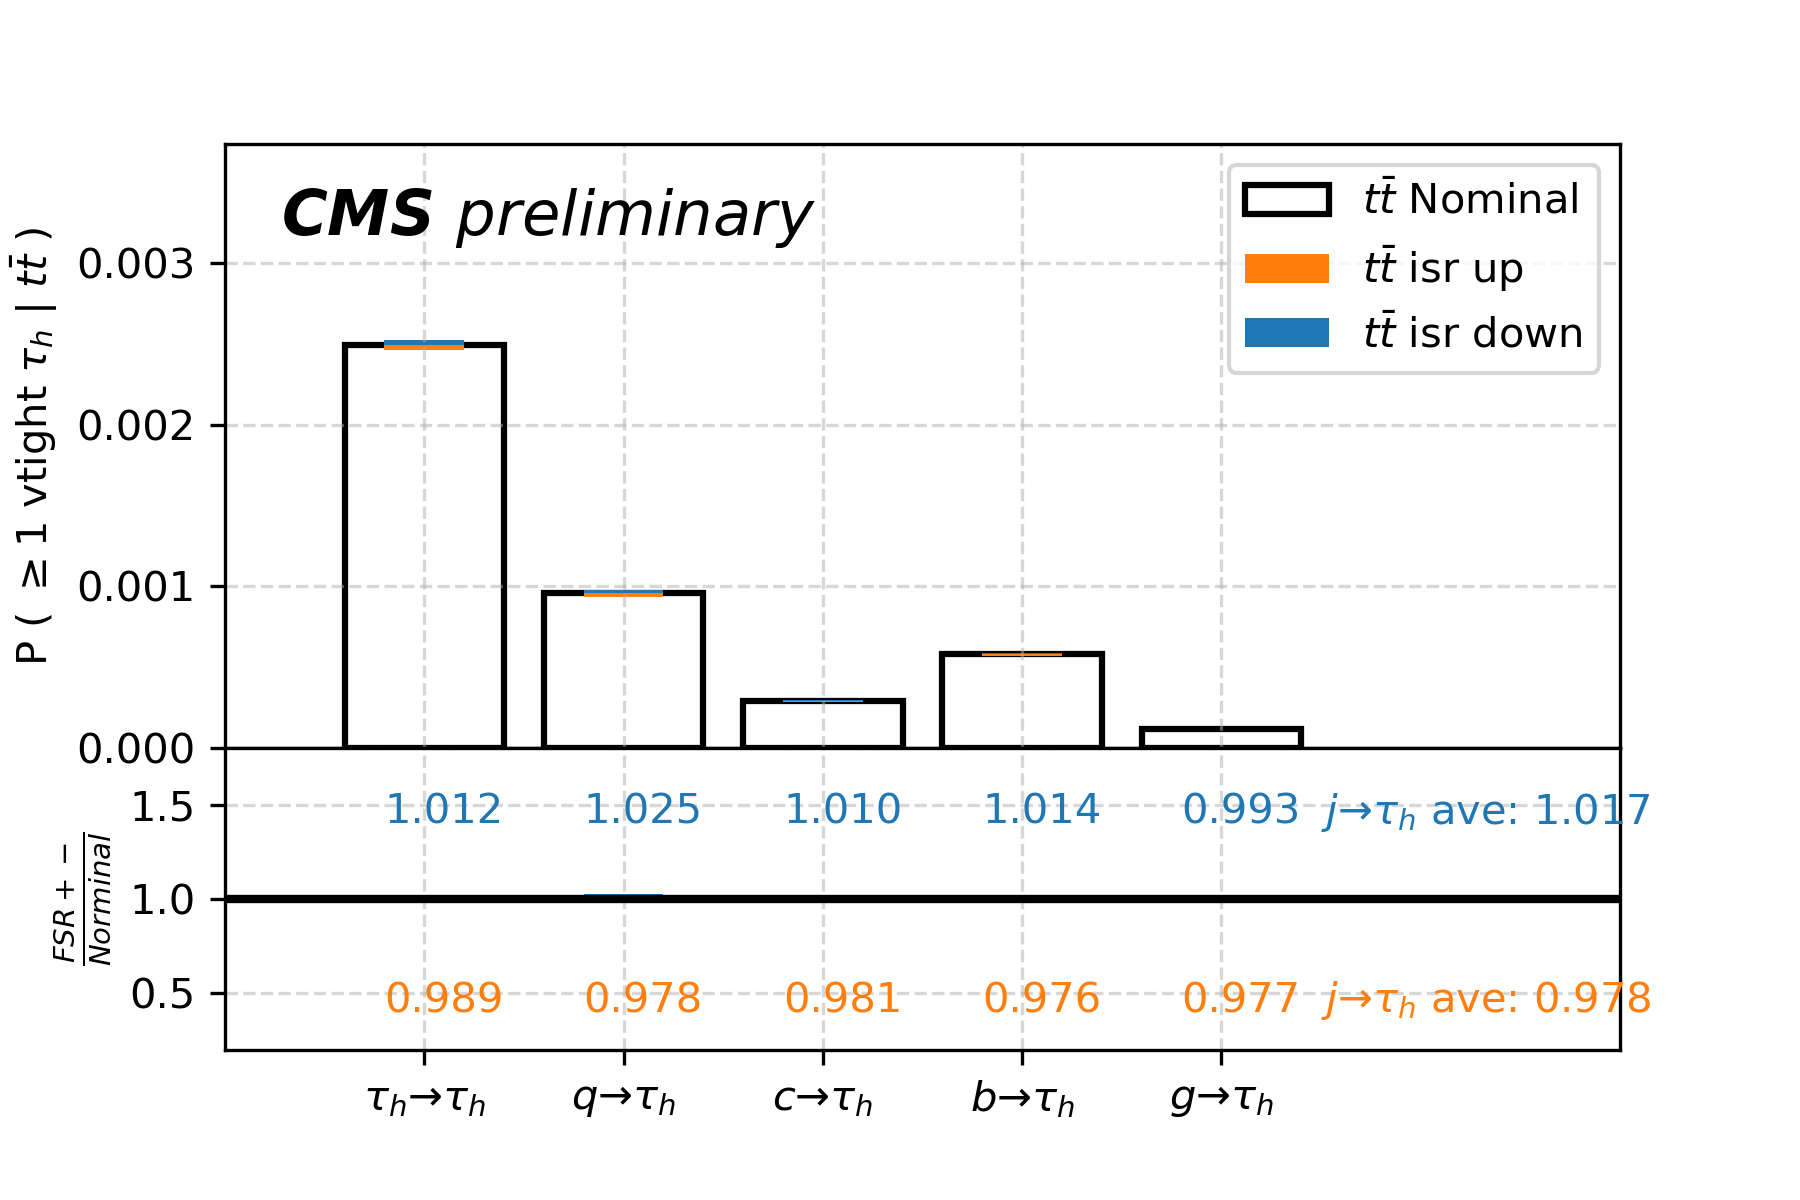
\includegraphics[width=0.49\textwidth]{chapters/Appendix/sectionTTSyst/figures/2020_MCRatio_isr_tauGenFlavor_tauVTight.png}
    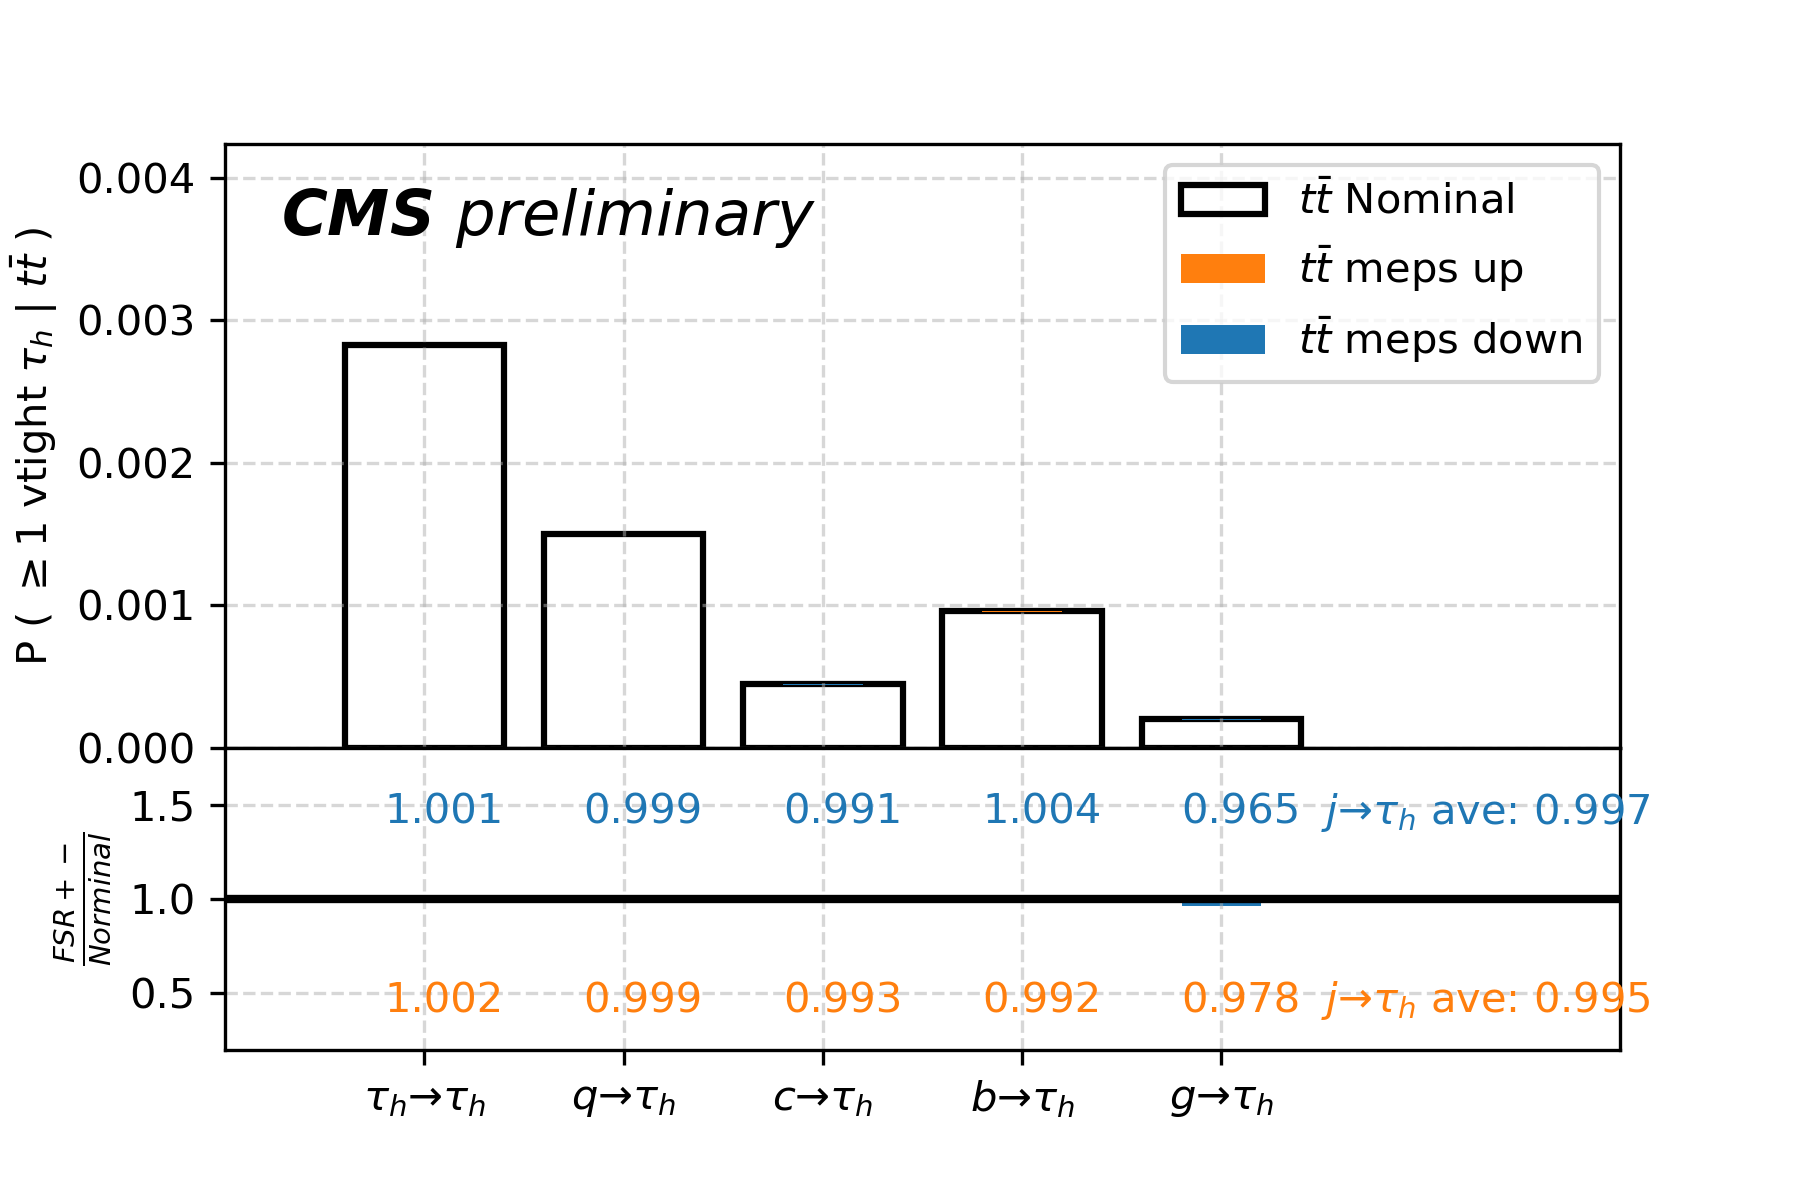
\includegraphics[width=0.49\textwidth]{chapters/Appendix/sectionTTSyst/figures/2020_MCRatio_meps_tauGenFlavor_tauTight.png}
    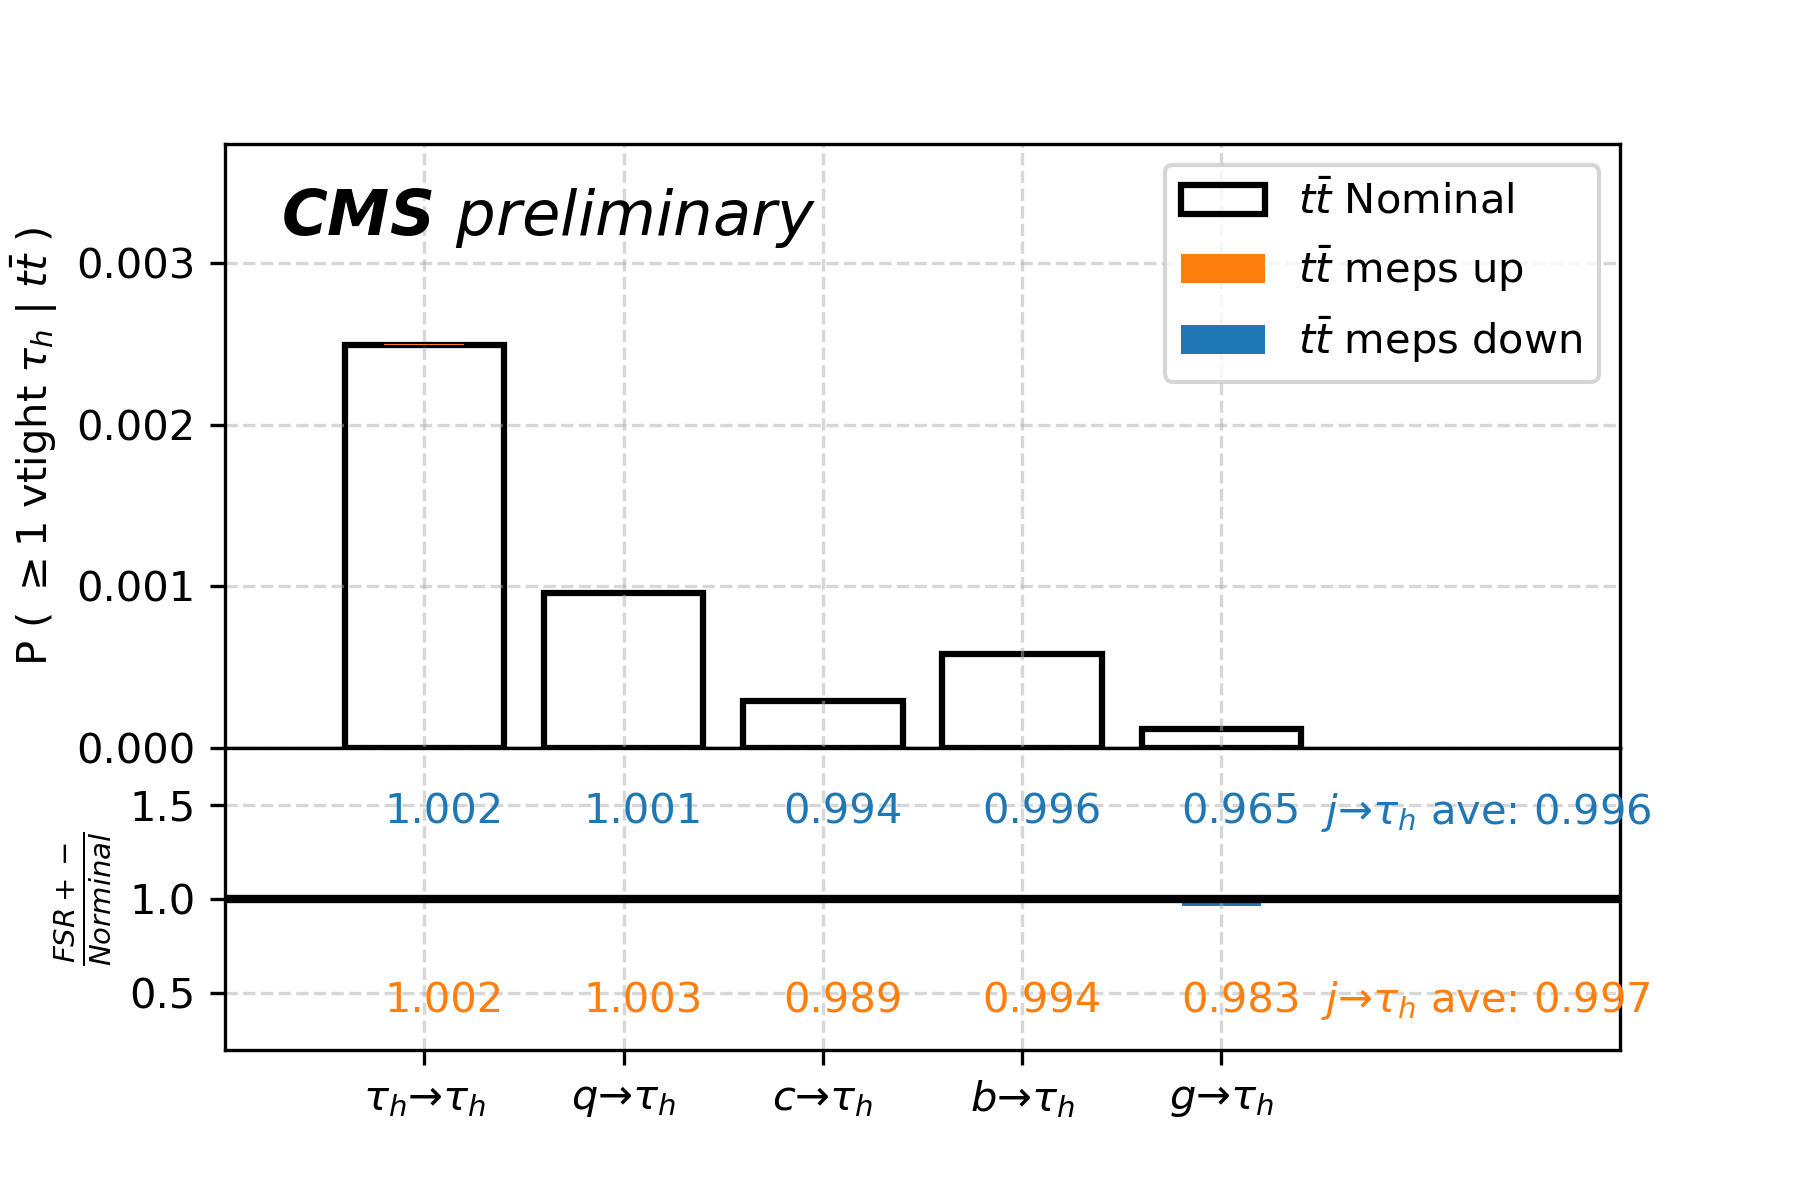
\includegraphics[width=0.49\textwidth]{chapters/Appendix/sectionTTSyst/figures/2020_MCRatio_meps_tauGenFlavor_tauVTight.png}
    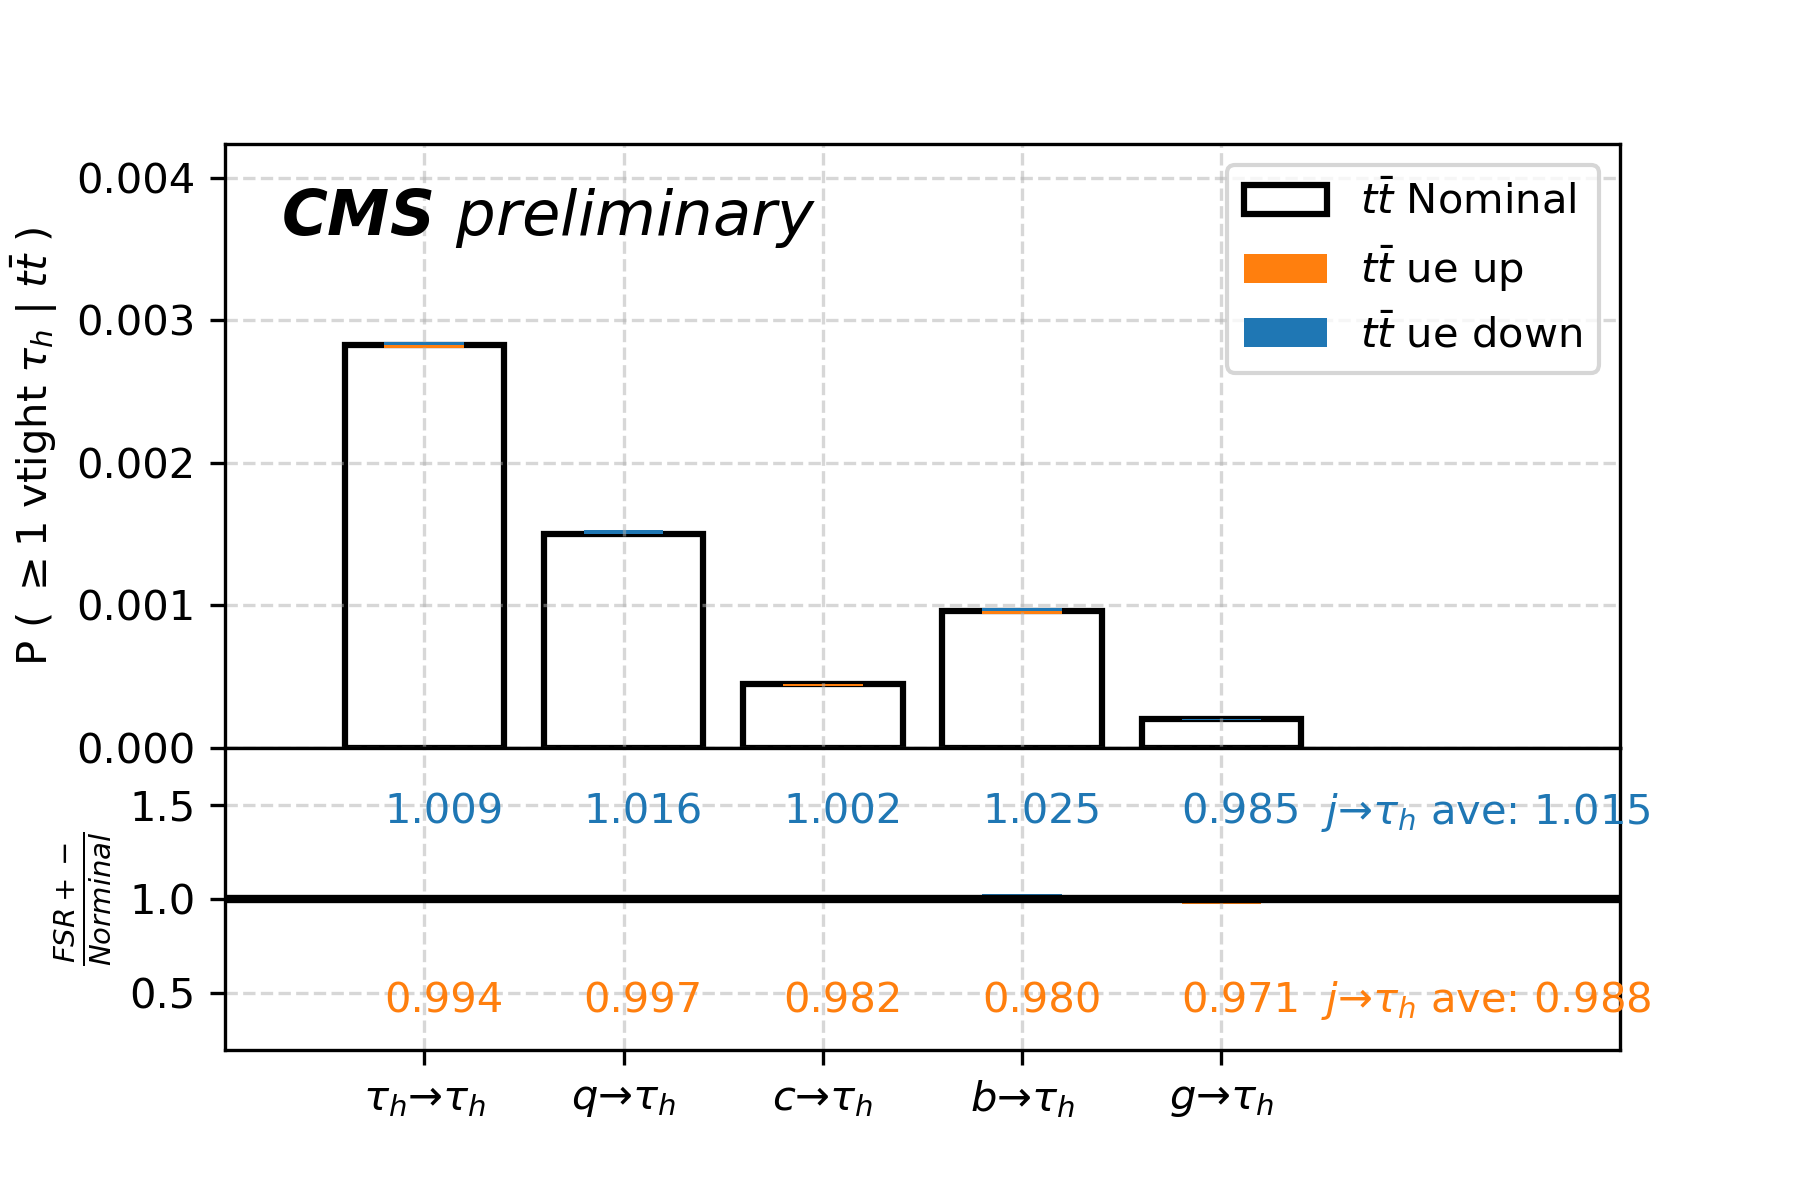
\includegraphics[width=0.49\textwidth]{chapters/Appendix/sectionTTSyst/figures/2020_MCRatio_ue_tauGenFlavor_tauTight.png}
    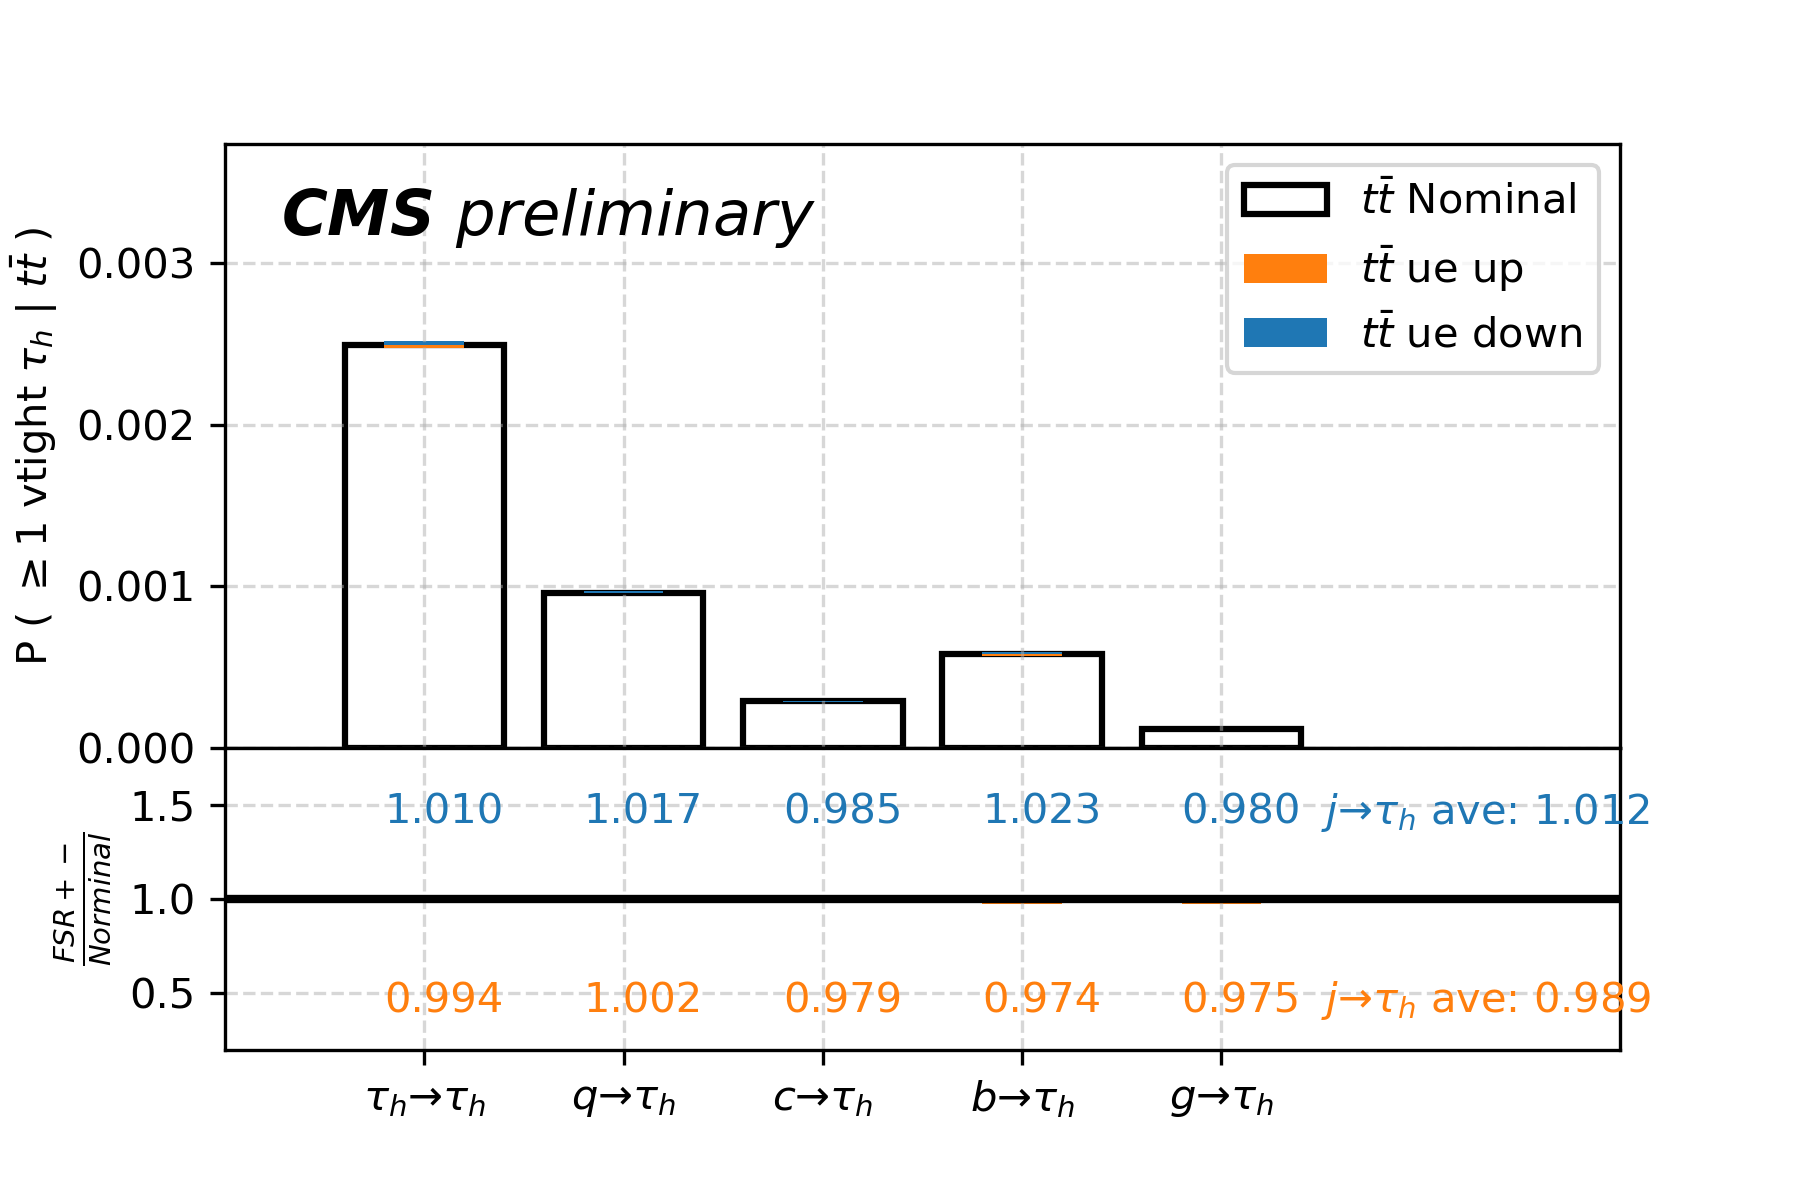
\includegraphics[width=0.49\textwidth]{chapters/Appendix/sectionTTSyst/figures/2020_MCRatio_ue_tauGenFlavor_tauVTight.png}
    \caption{Reweight $\tau_h$ and $j \to \tau_h$ efficiencies in the dedicated ISF, MEPS, UE ttbar samples}
    \label{fig:appendix:reweighttt:sf}
\end{figure}


\begin{figure}
    \centering
    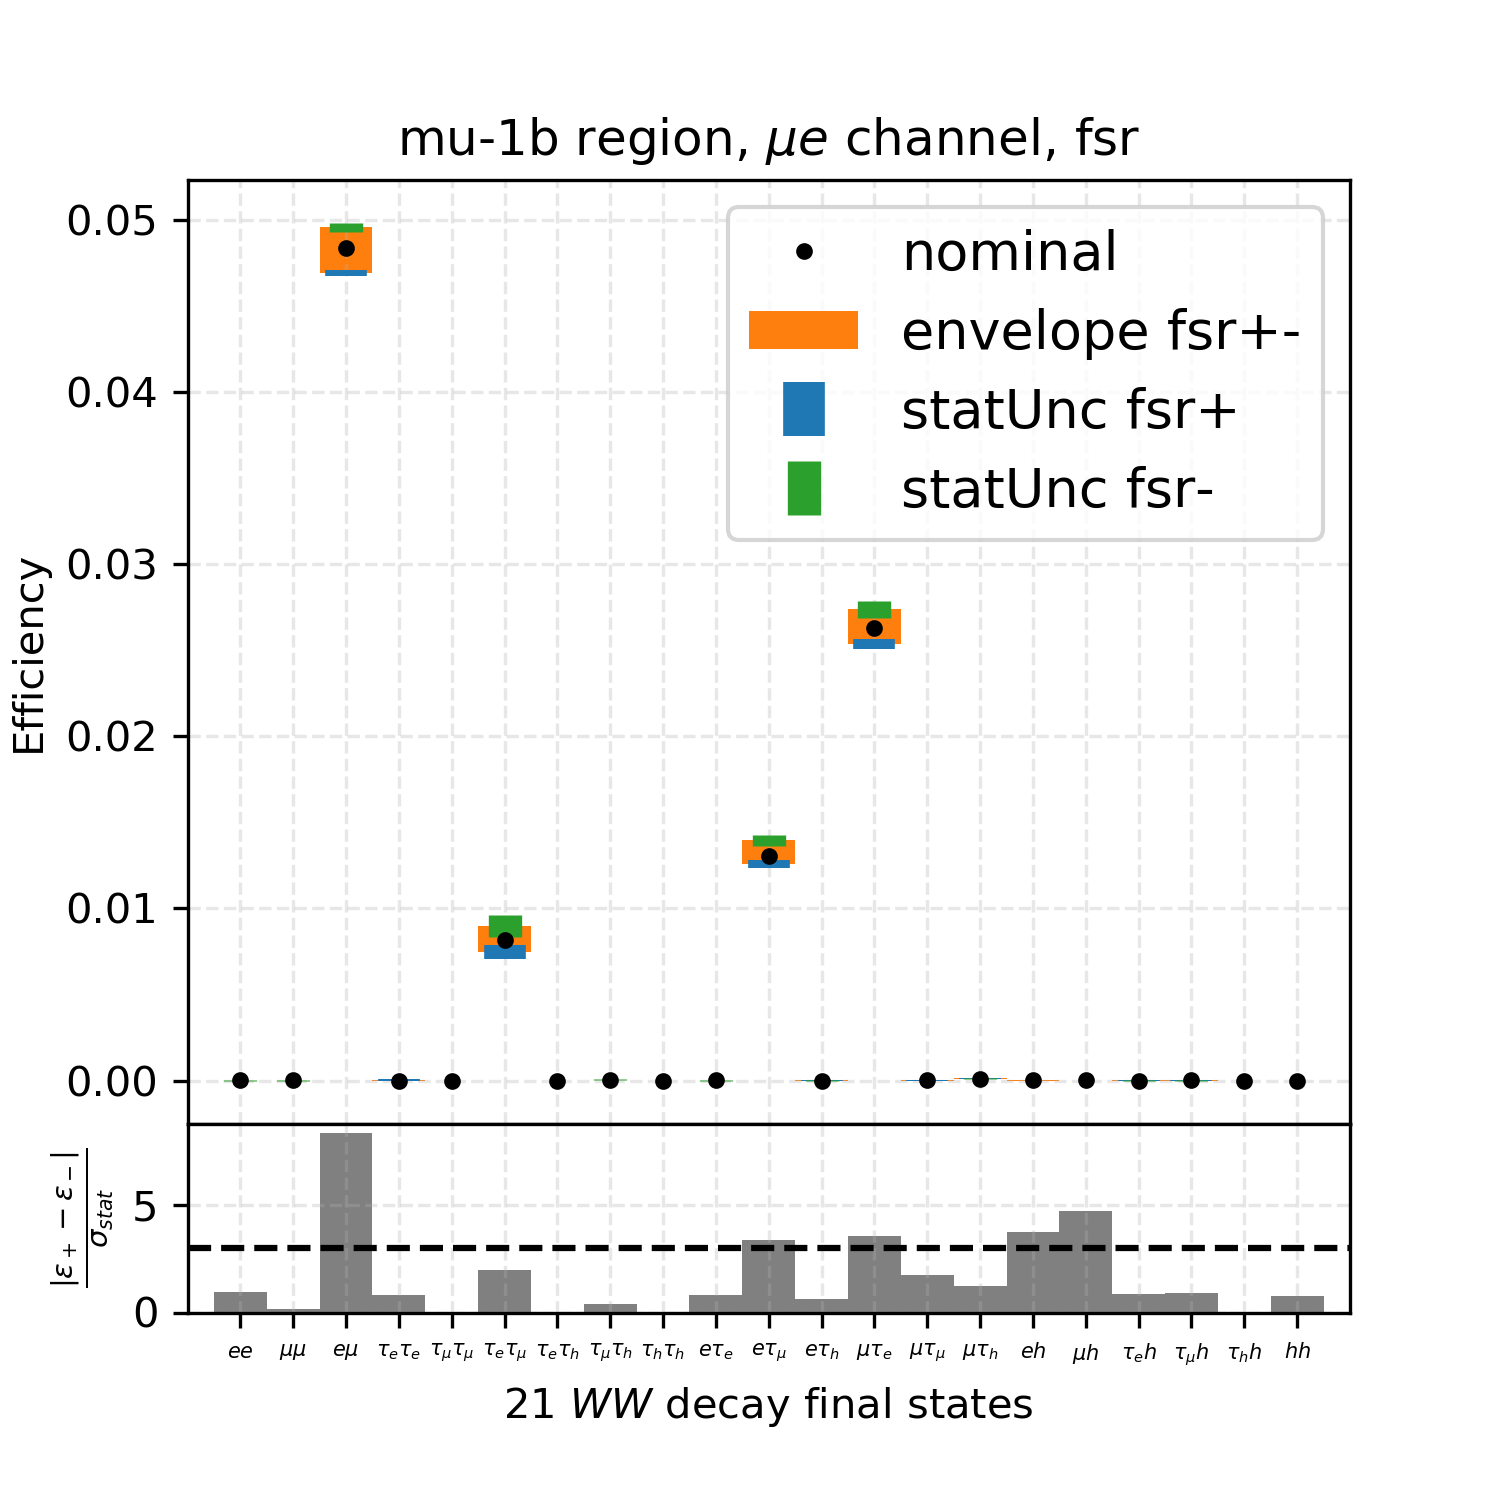
\includegraphics[width=0.24\textwidth]{chapters/Appendix/sectionTTSyst/figures/afterCorr/icata0_ch0_fsr.png}
    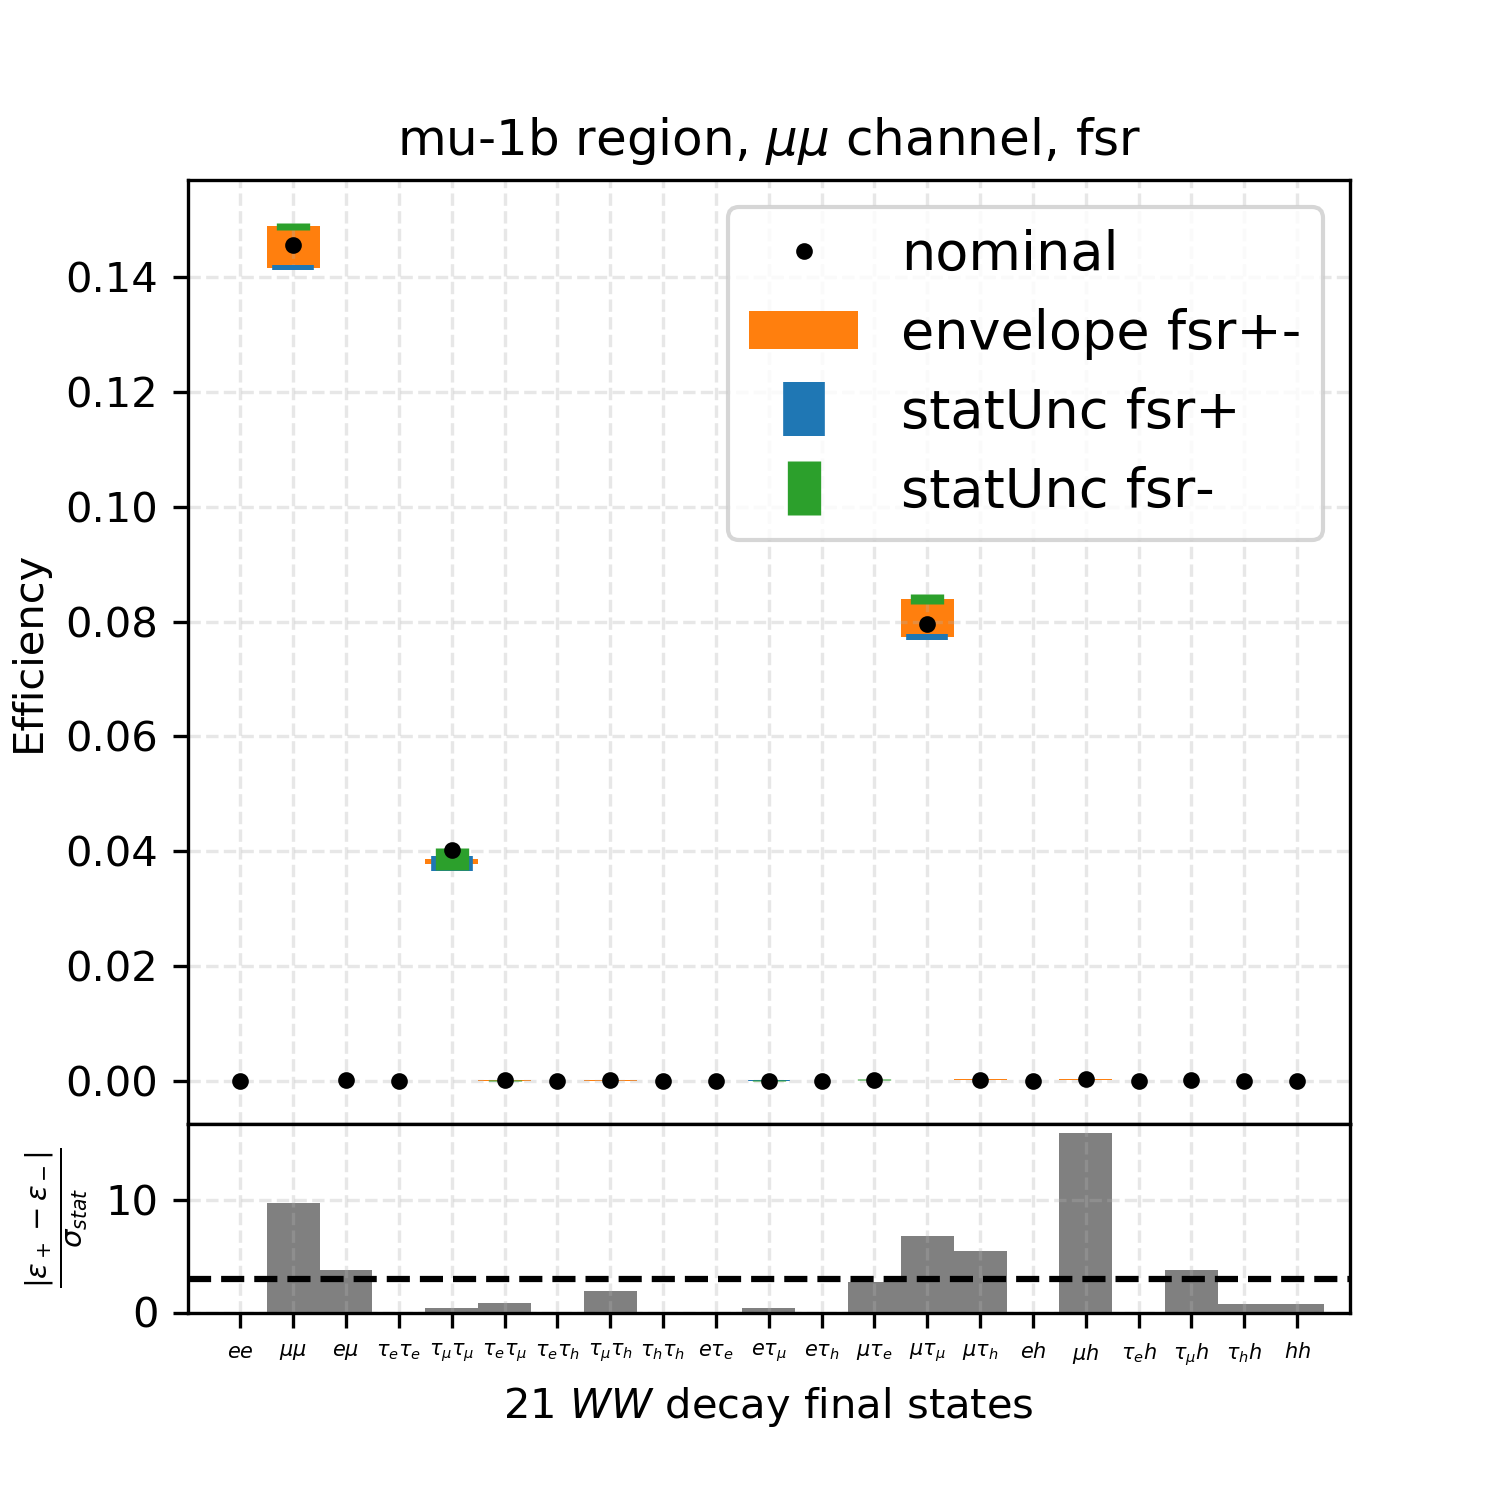
\includegraphics[width=0.24\textwidth]{chapters/Appendix/sectionTTSyst/figures/afterCorr/icata0_ch1_fsr.png}
    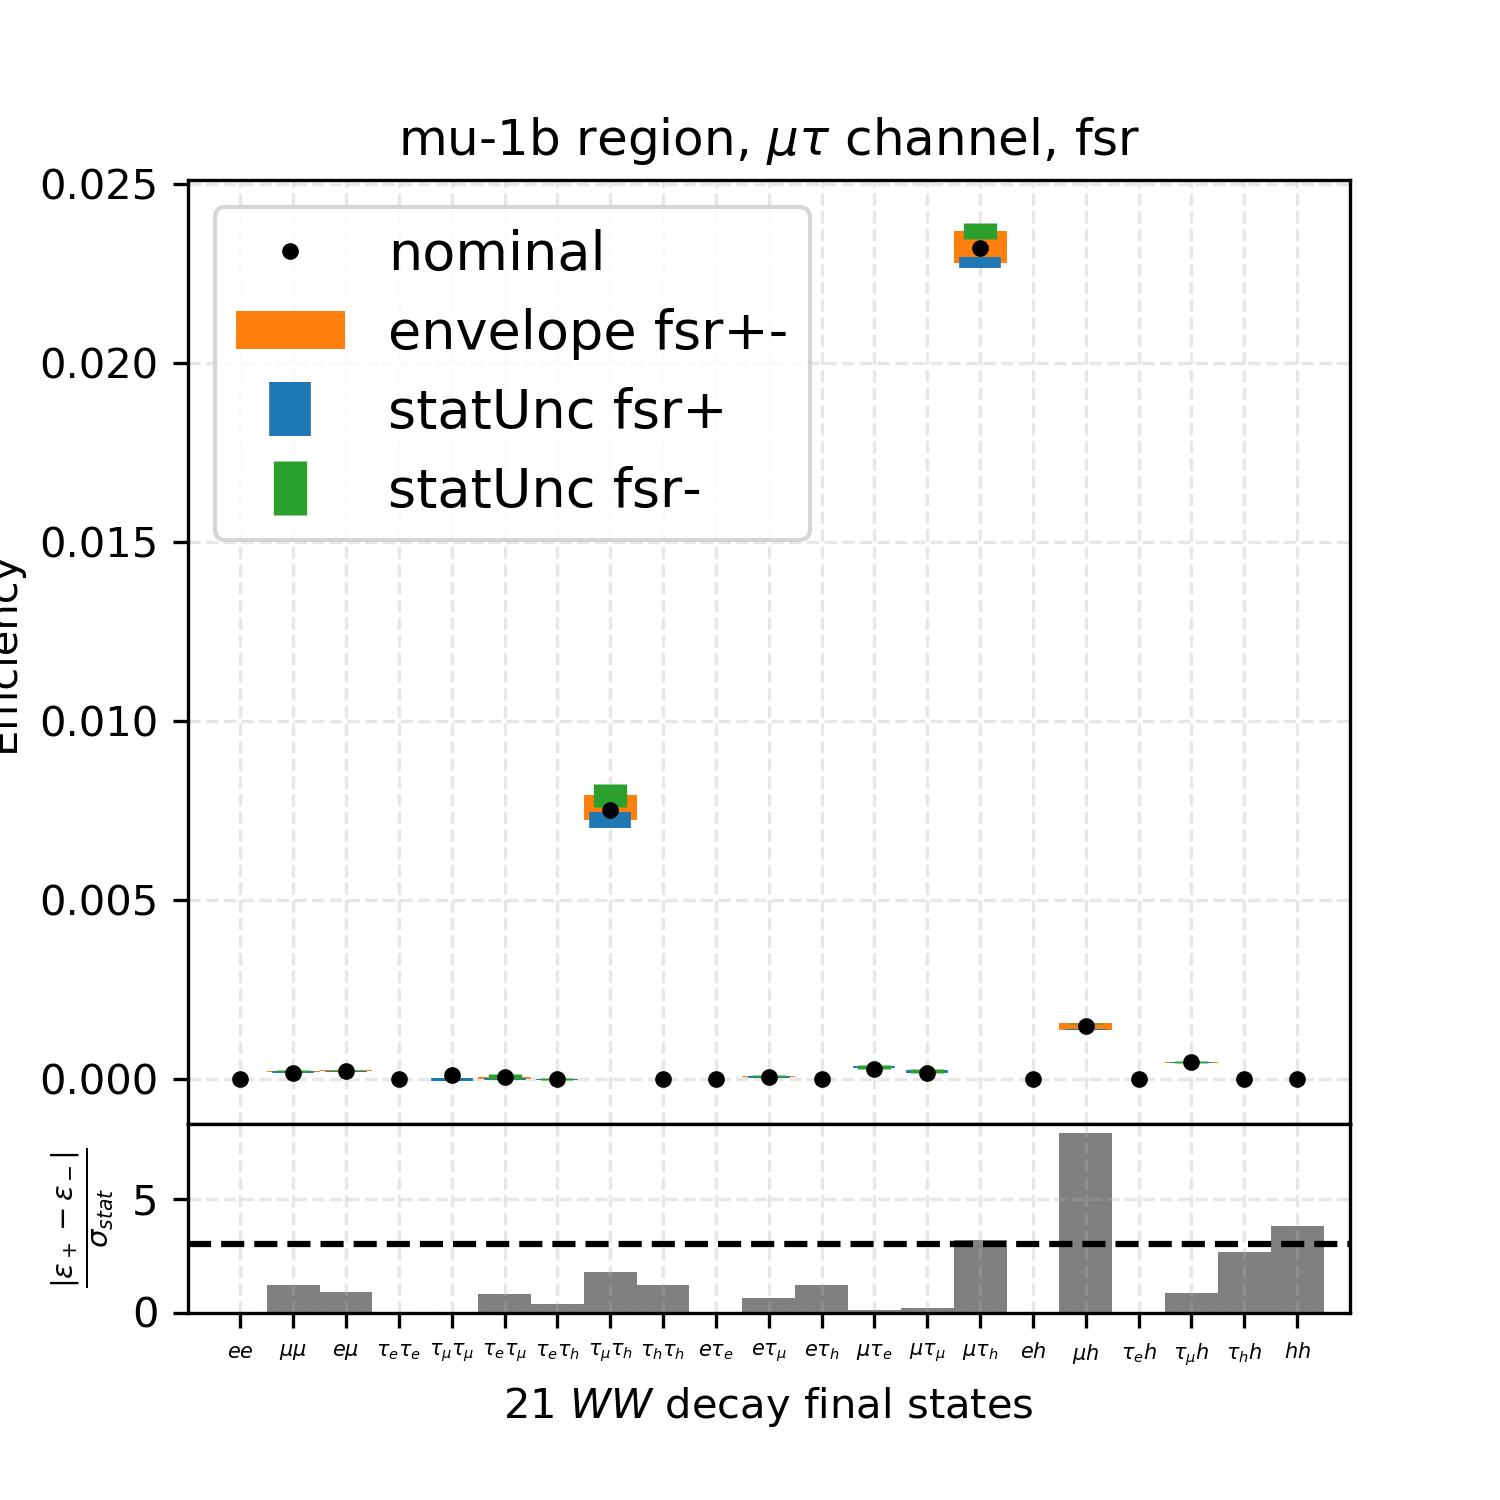
\includegraphics[width=0.24\textwidth]{chapters/Appendix/sectionTTSyst/figures/afterCorr/icata0_ch2_fsr.png}
    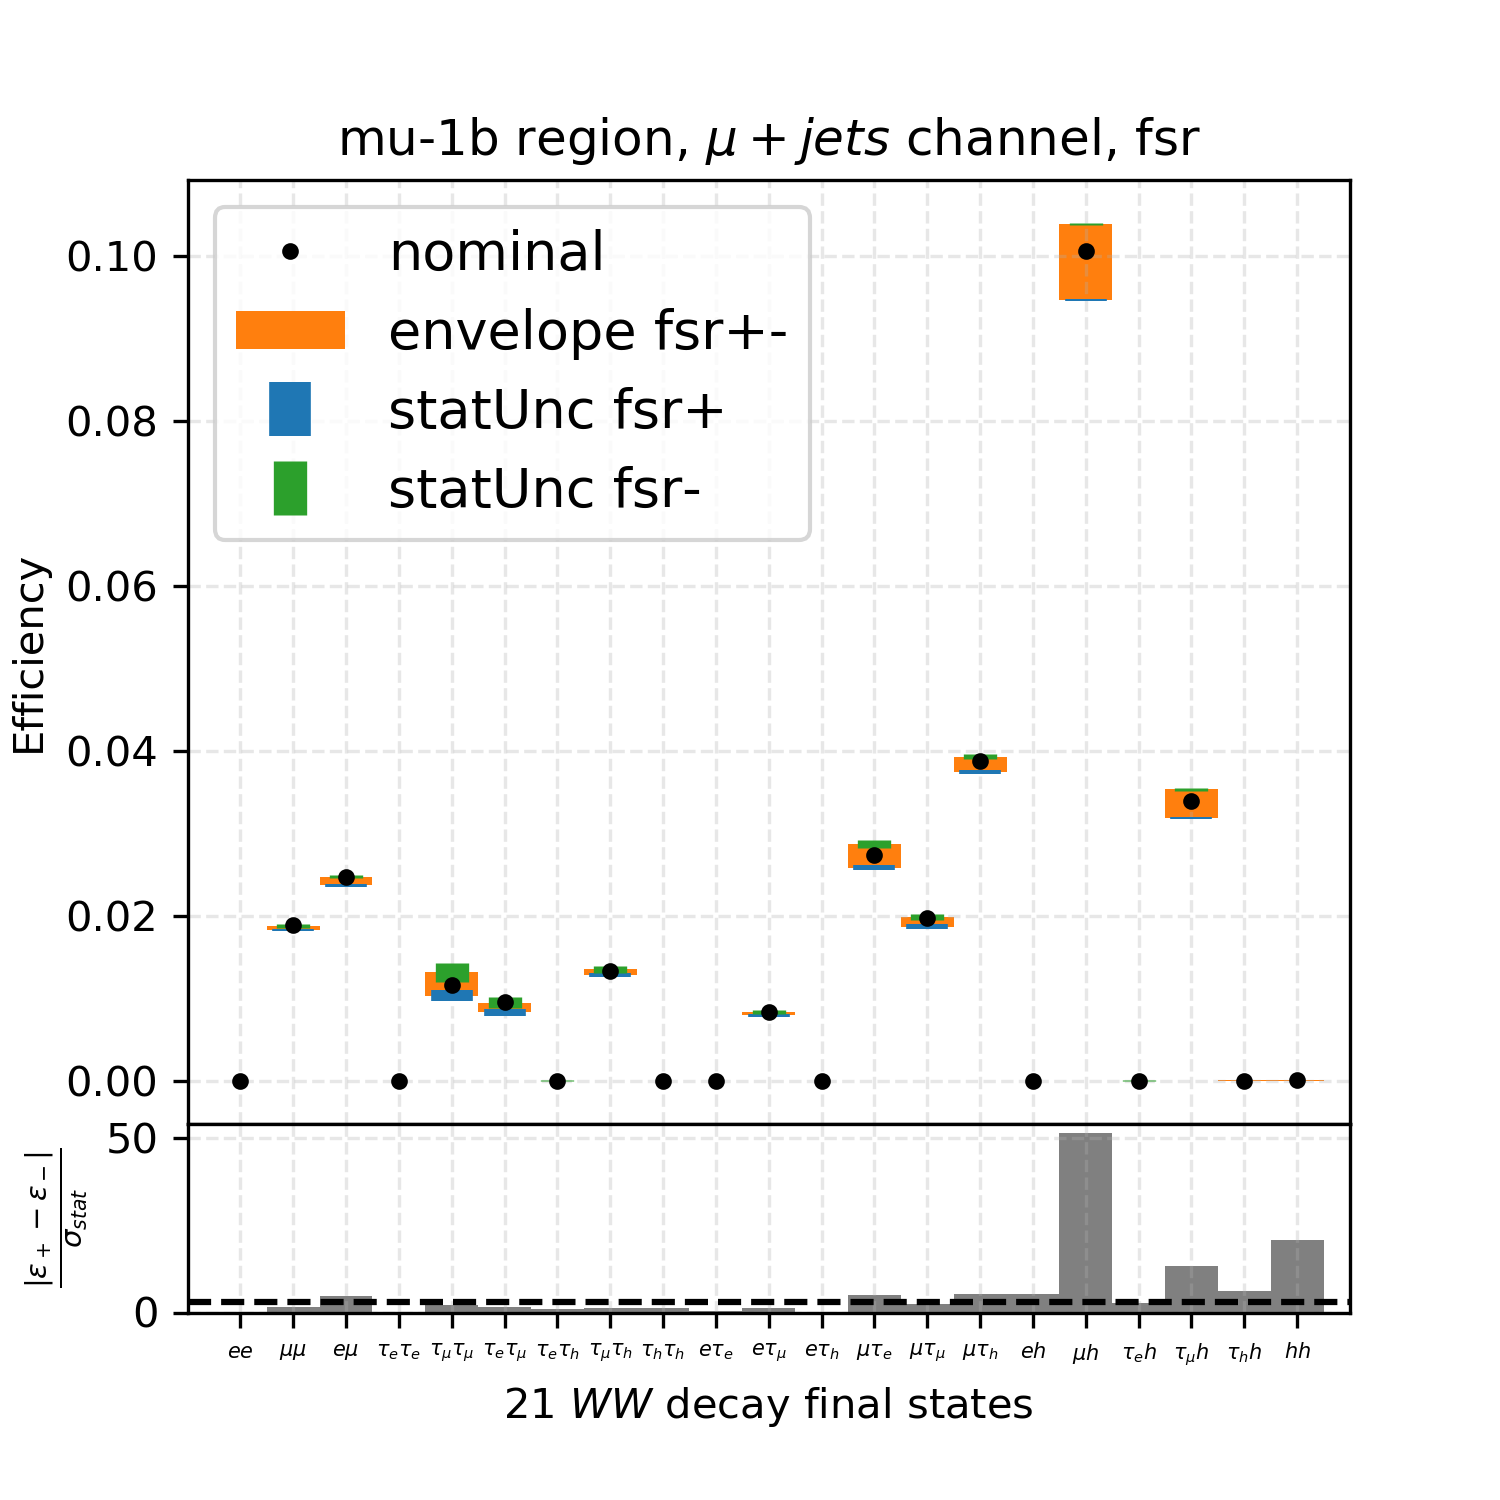
\includegraphics[width=0.24\textwidth]{chapters/Appendix/sectionTTSyst/figures/afterCorr/icata0_ch3_fsr.png}

    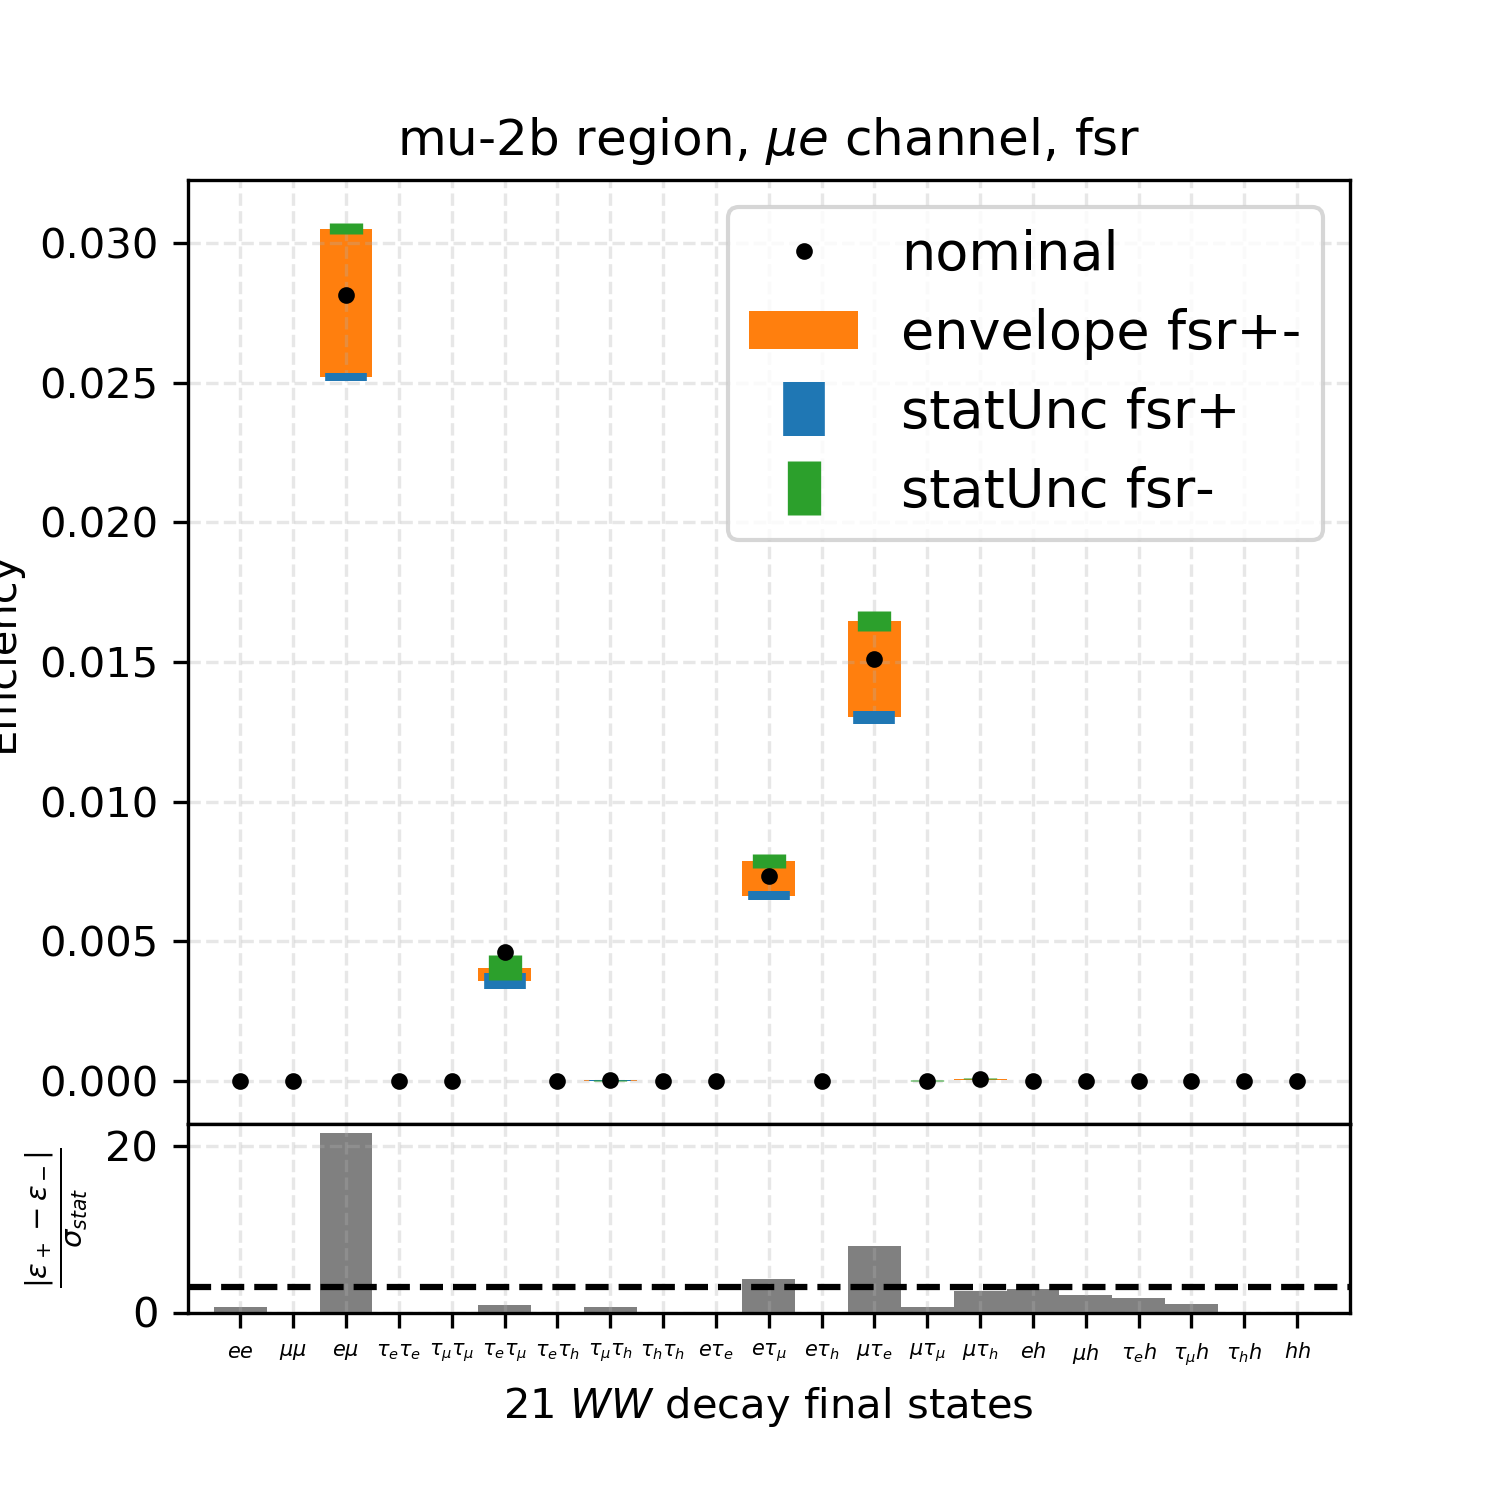
\includegraphics[width=0.24\textwidth]{chapters/Appendix/sectionTTSyst/figures/afterCorr/icata1_ch0_fsr.png}
    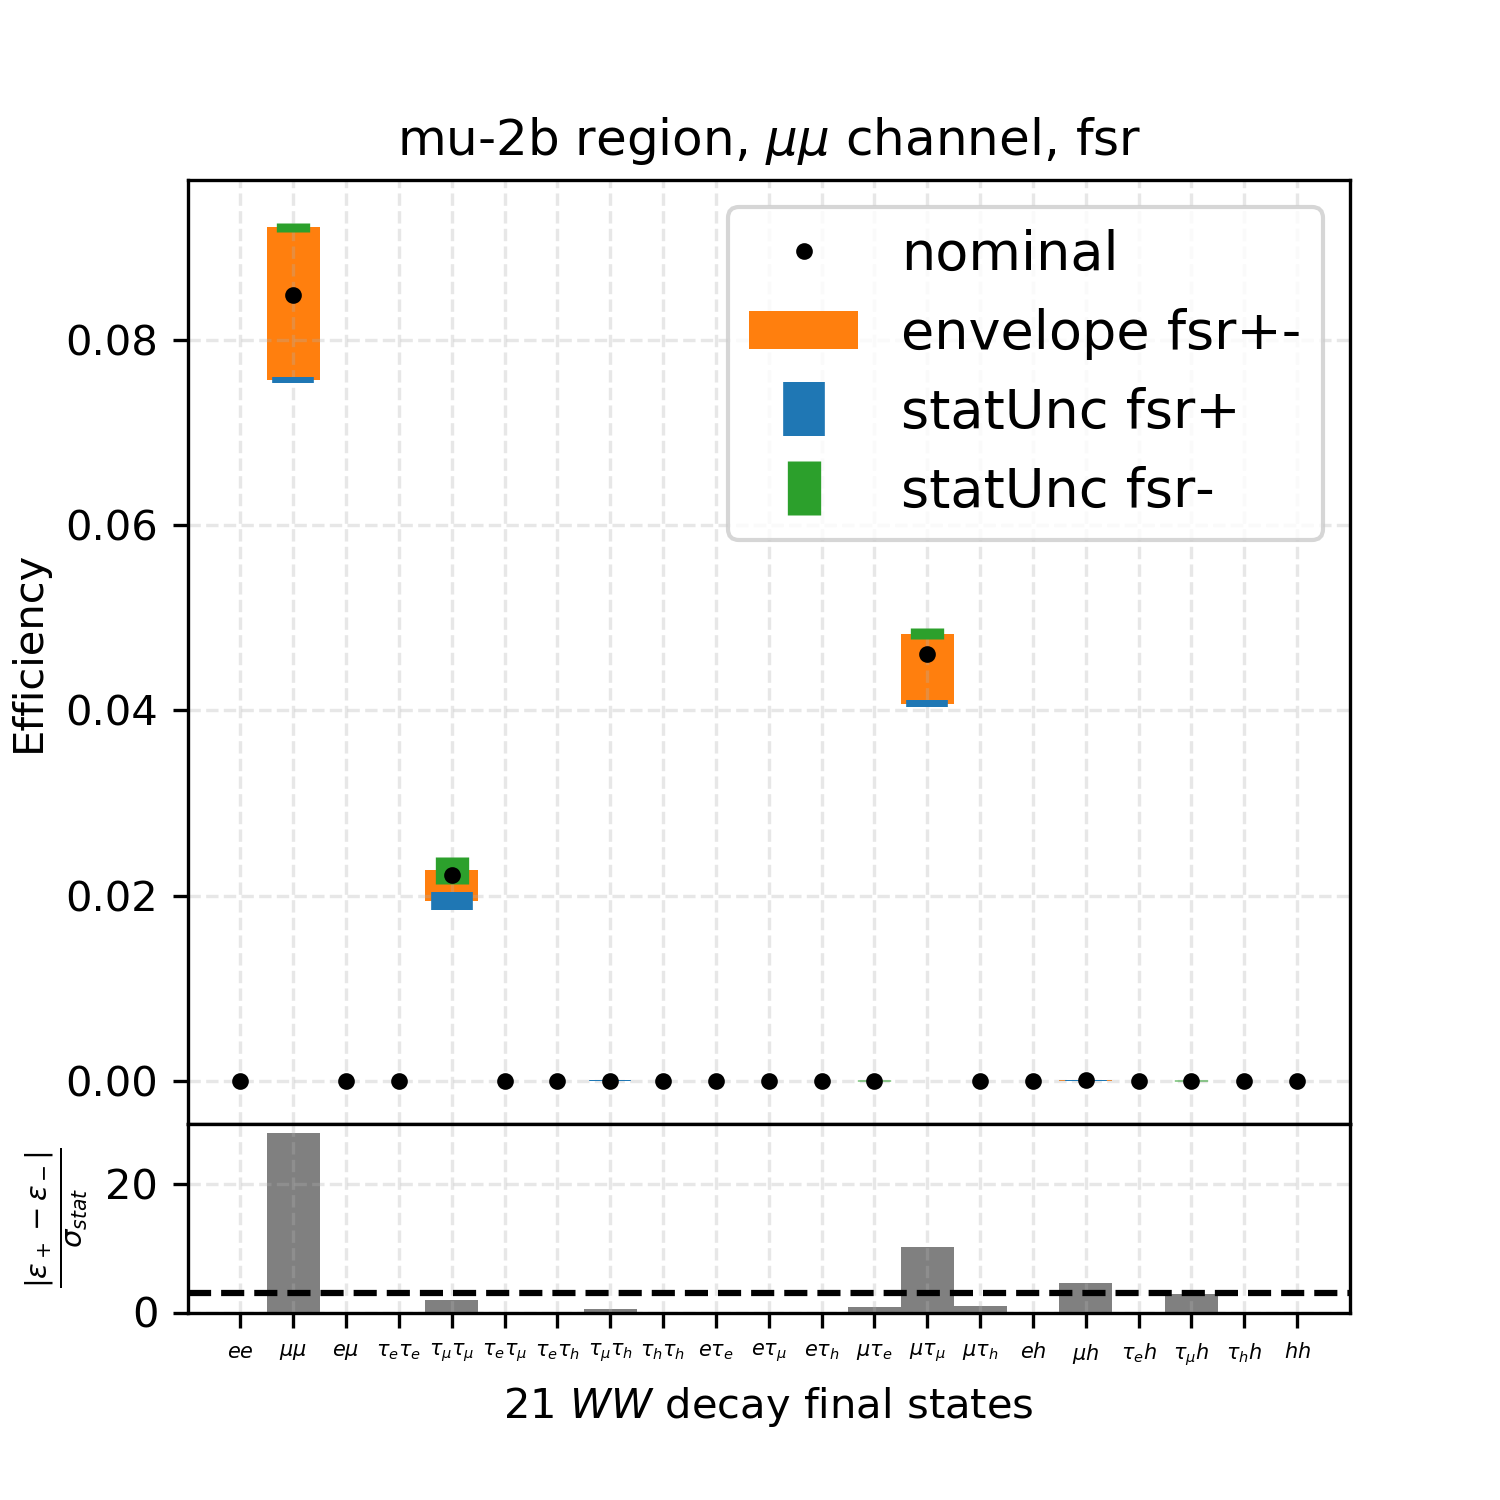
\includegraphics[width=0.24\textwidth]{chapters/Appendix/sectionTTSyst/figures/afterCorr/icata1_ch1_fsr.png}
    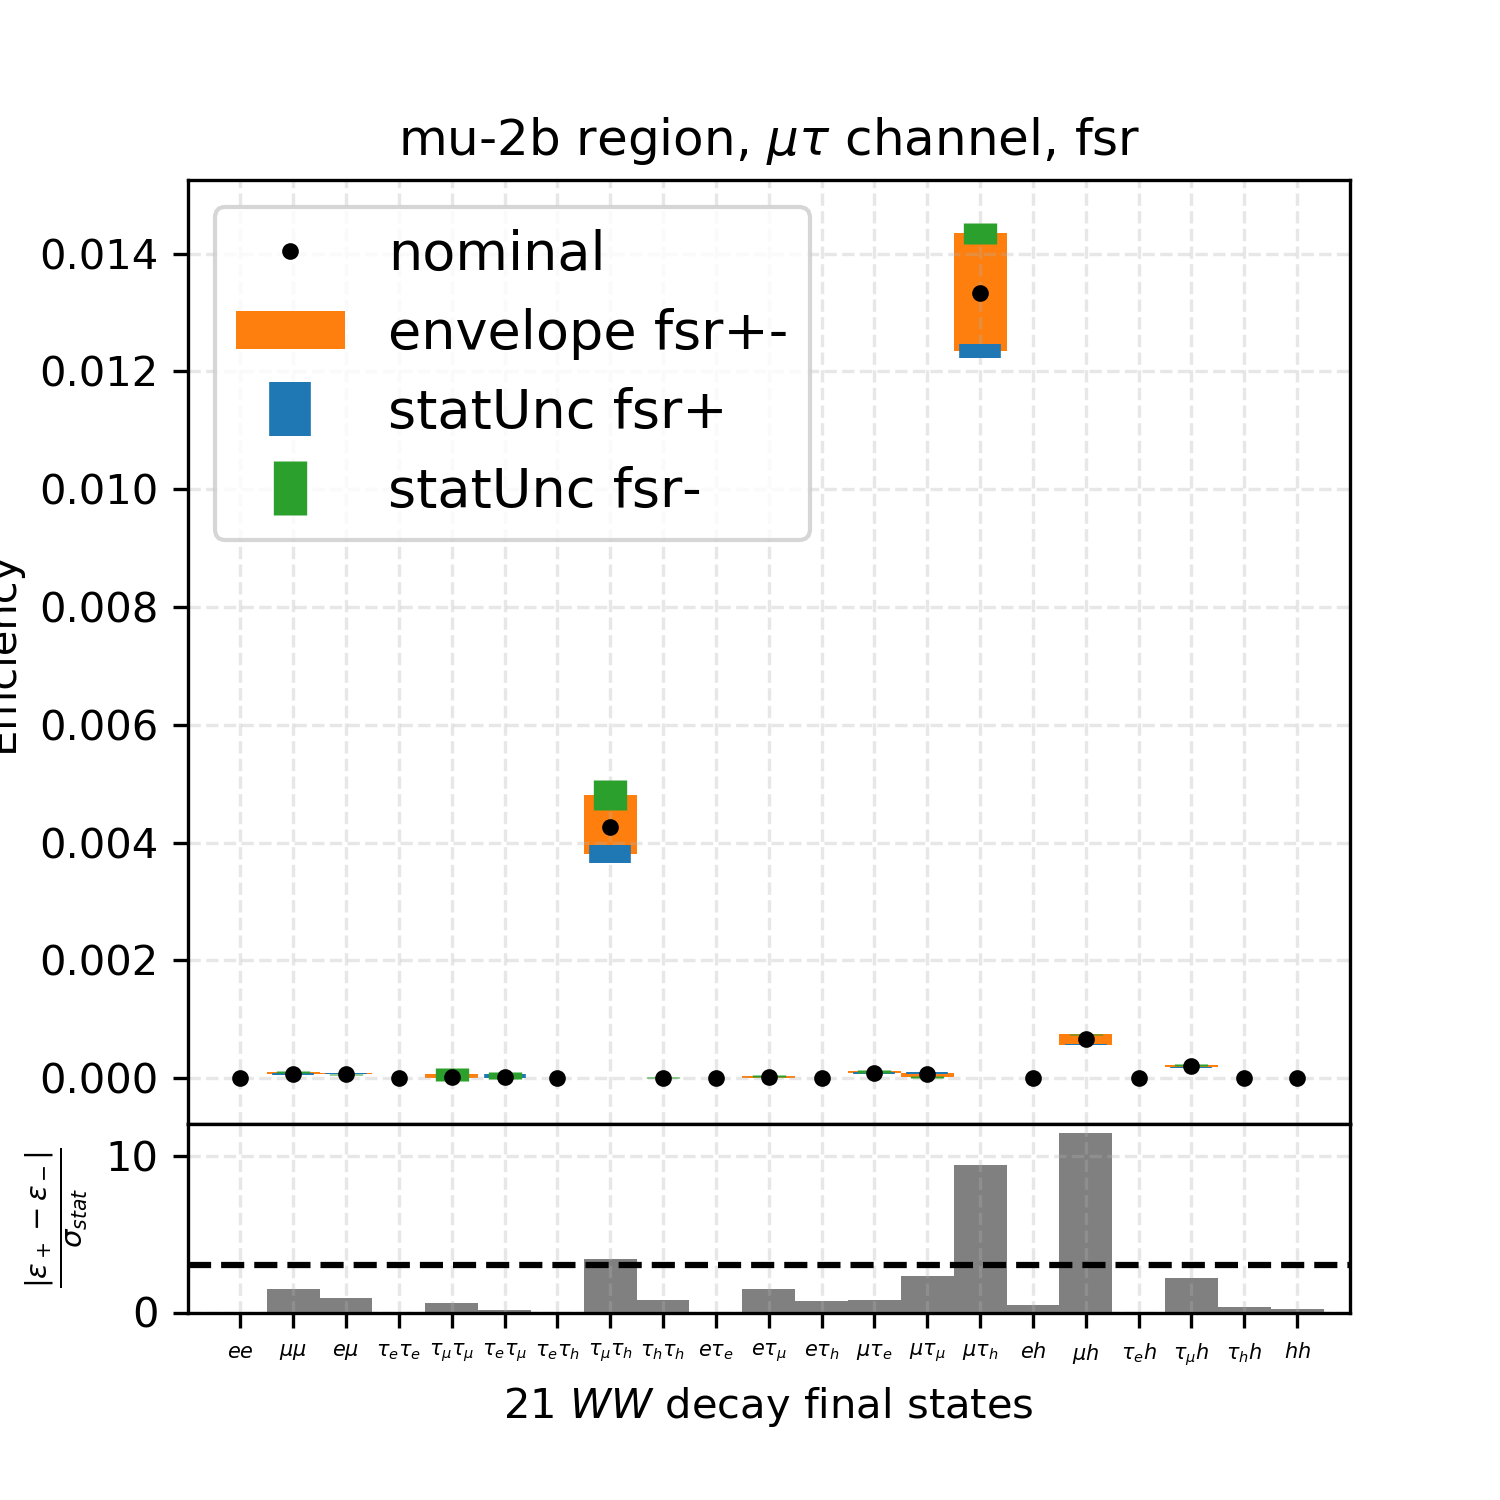
\includegraphics[width=0.24\textwidth]{chapters/Appendix/sectionTTSyst/figures/afterCorr/icata1_ch2_fsr.png}
    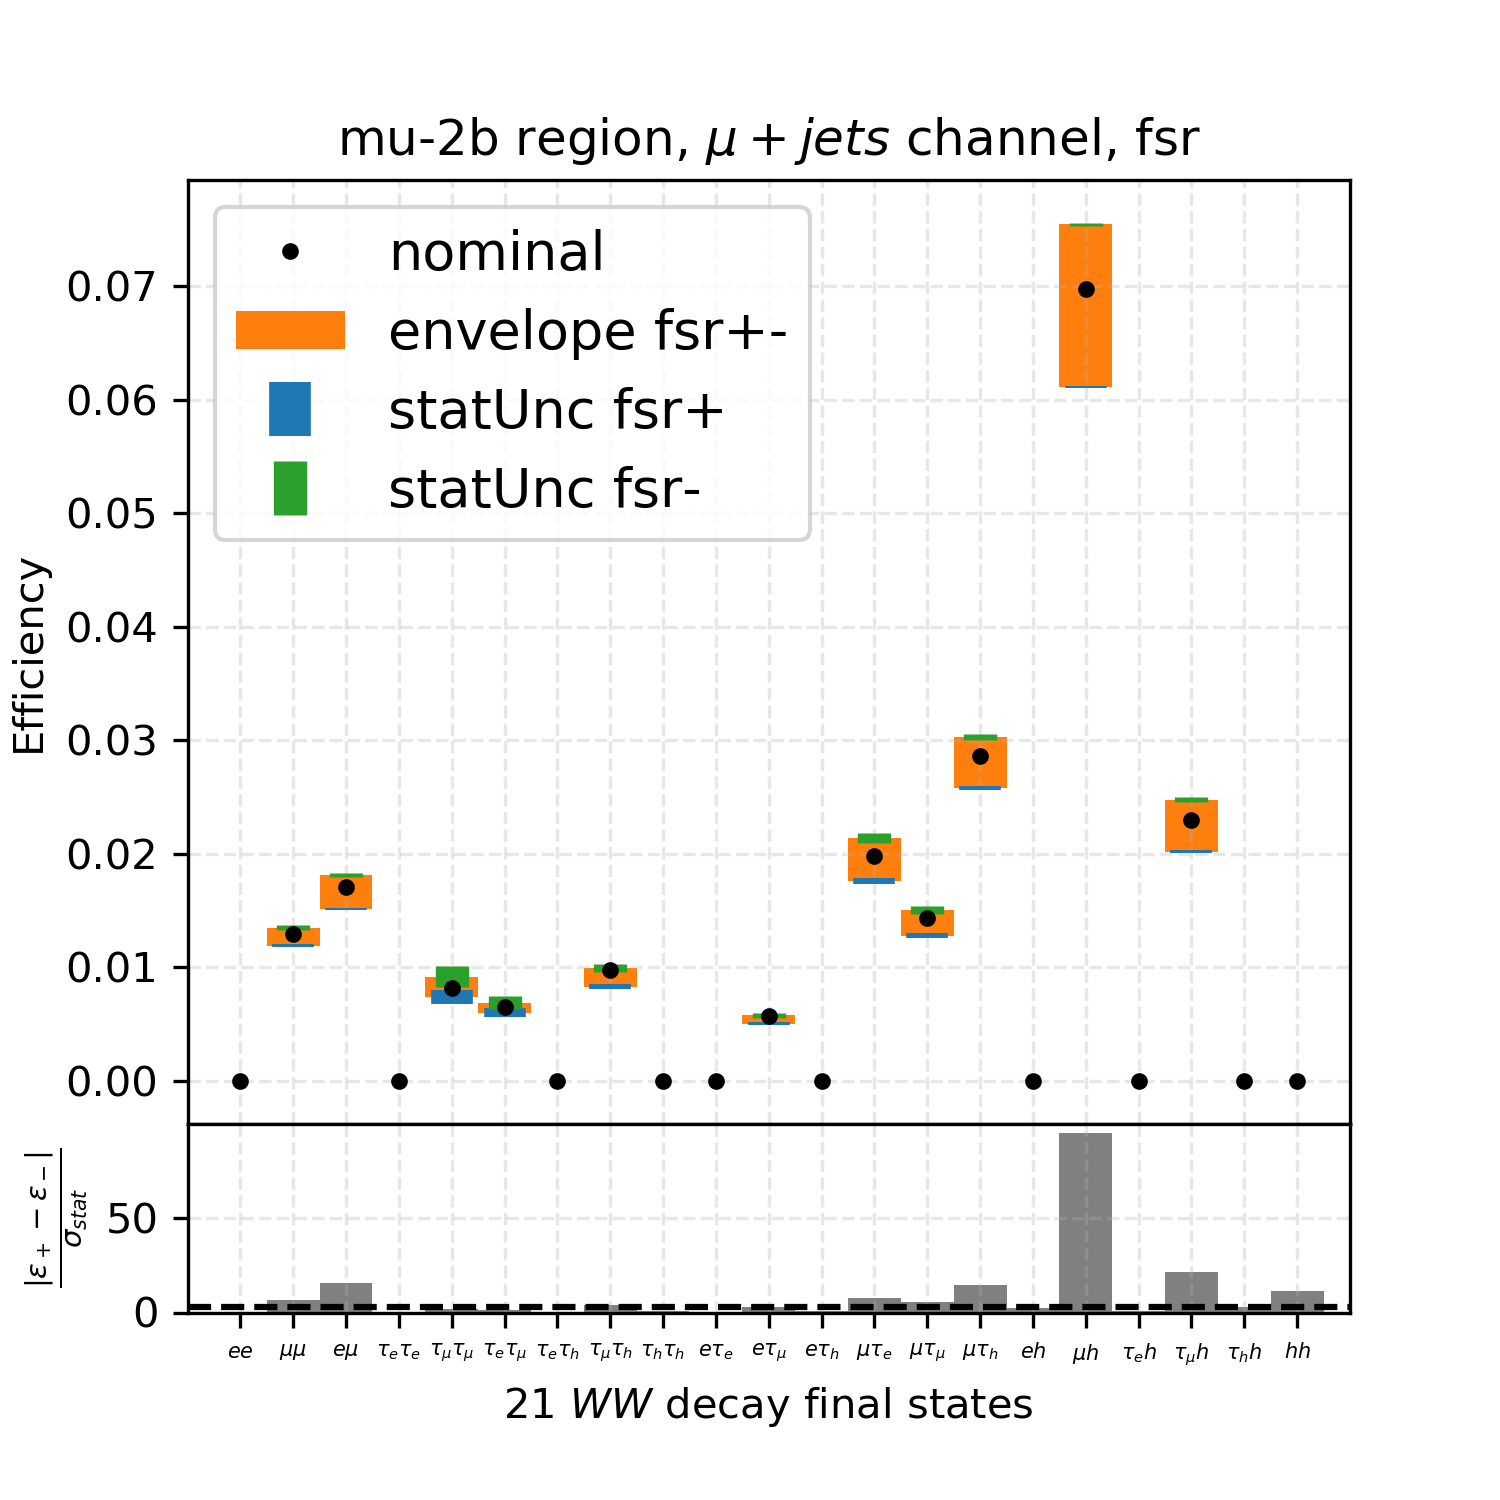
\includegraphics[width=0.24\textwidth]{chapters/Appendix/sectionTTSyst/figures/afterCorr/icata1_ch3_fsr.png}
    
    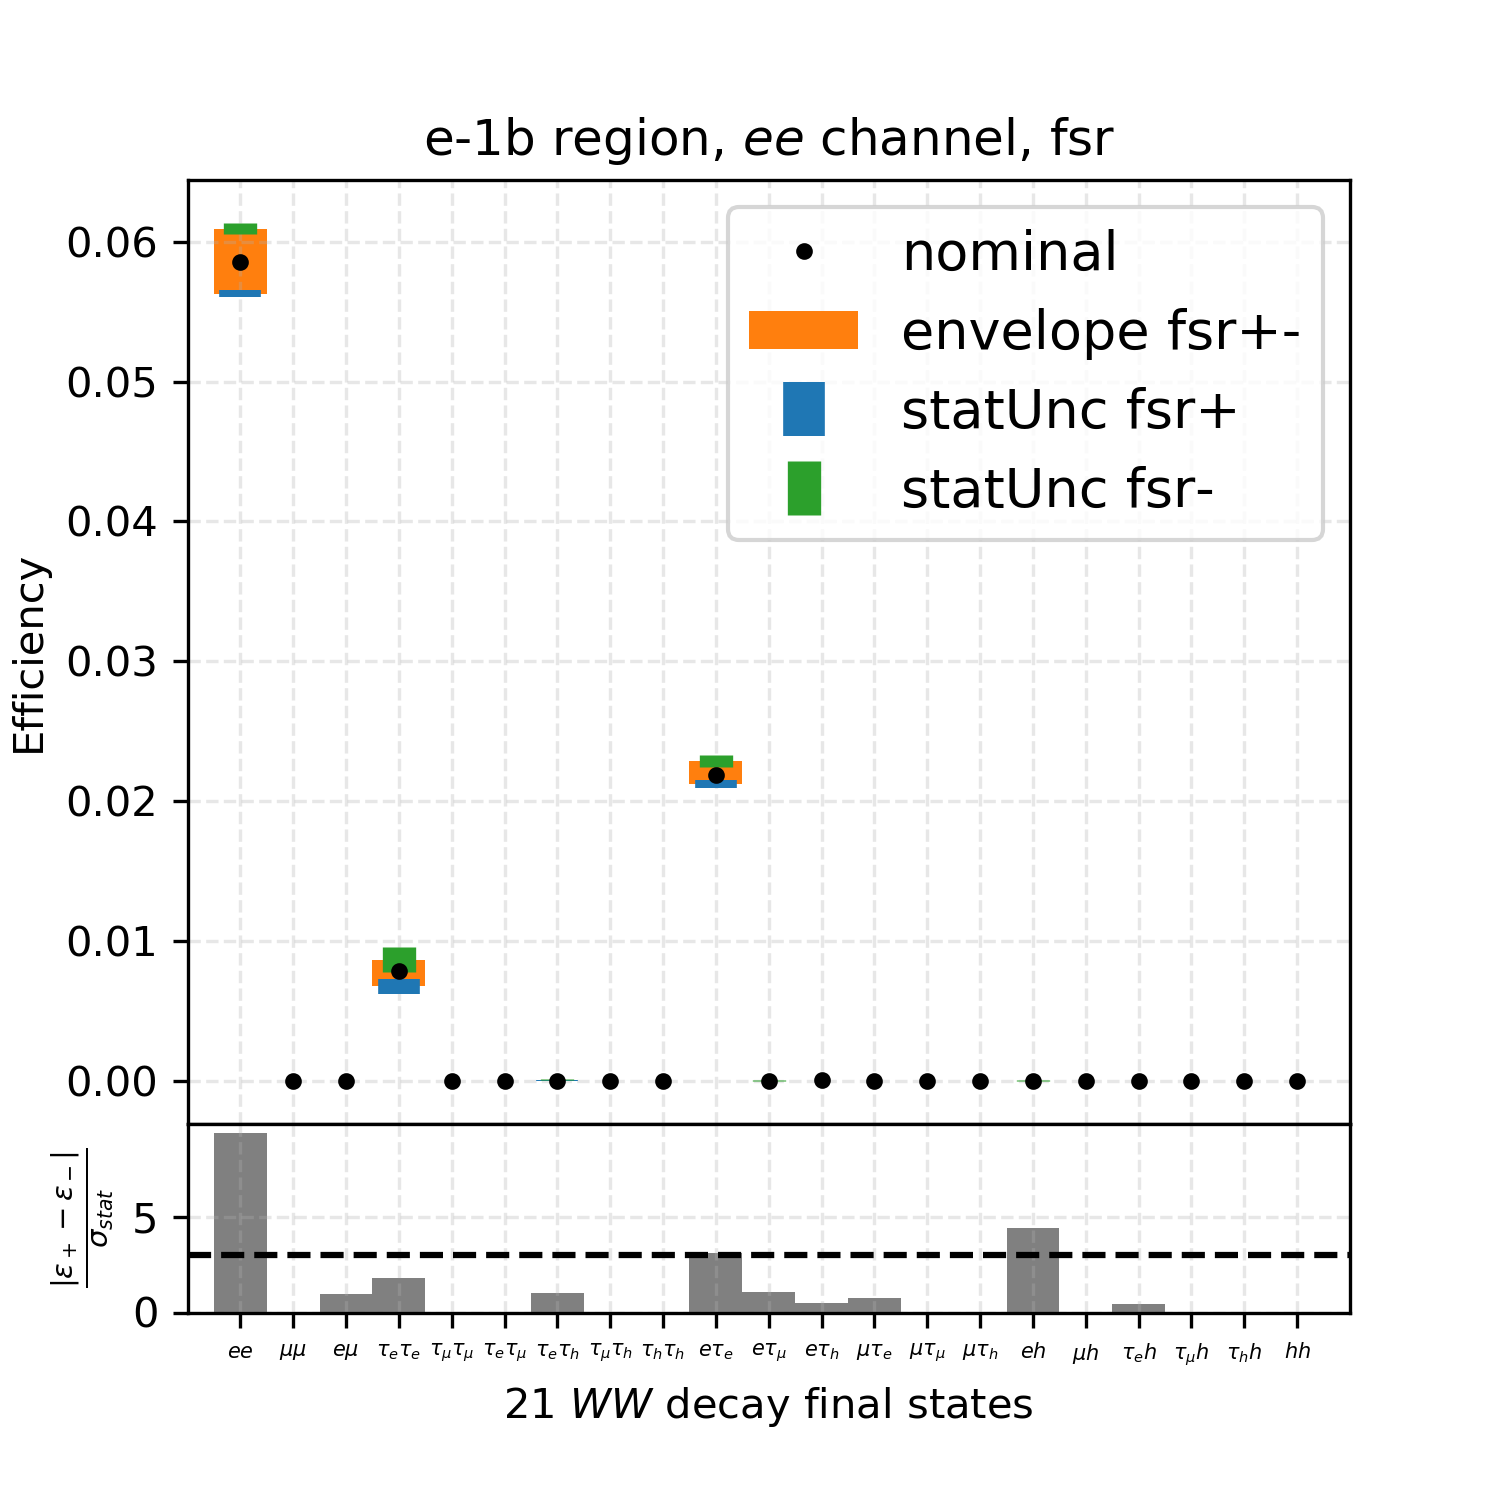
\includegraphics[width=0.24\textwidth]{chapters/Appendix/sectionTTSyst/figures/afterCorr/icata2_ch0_fsr.png}
    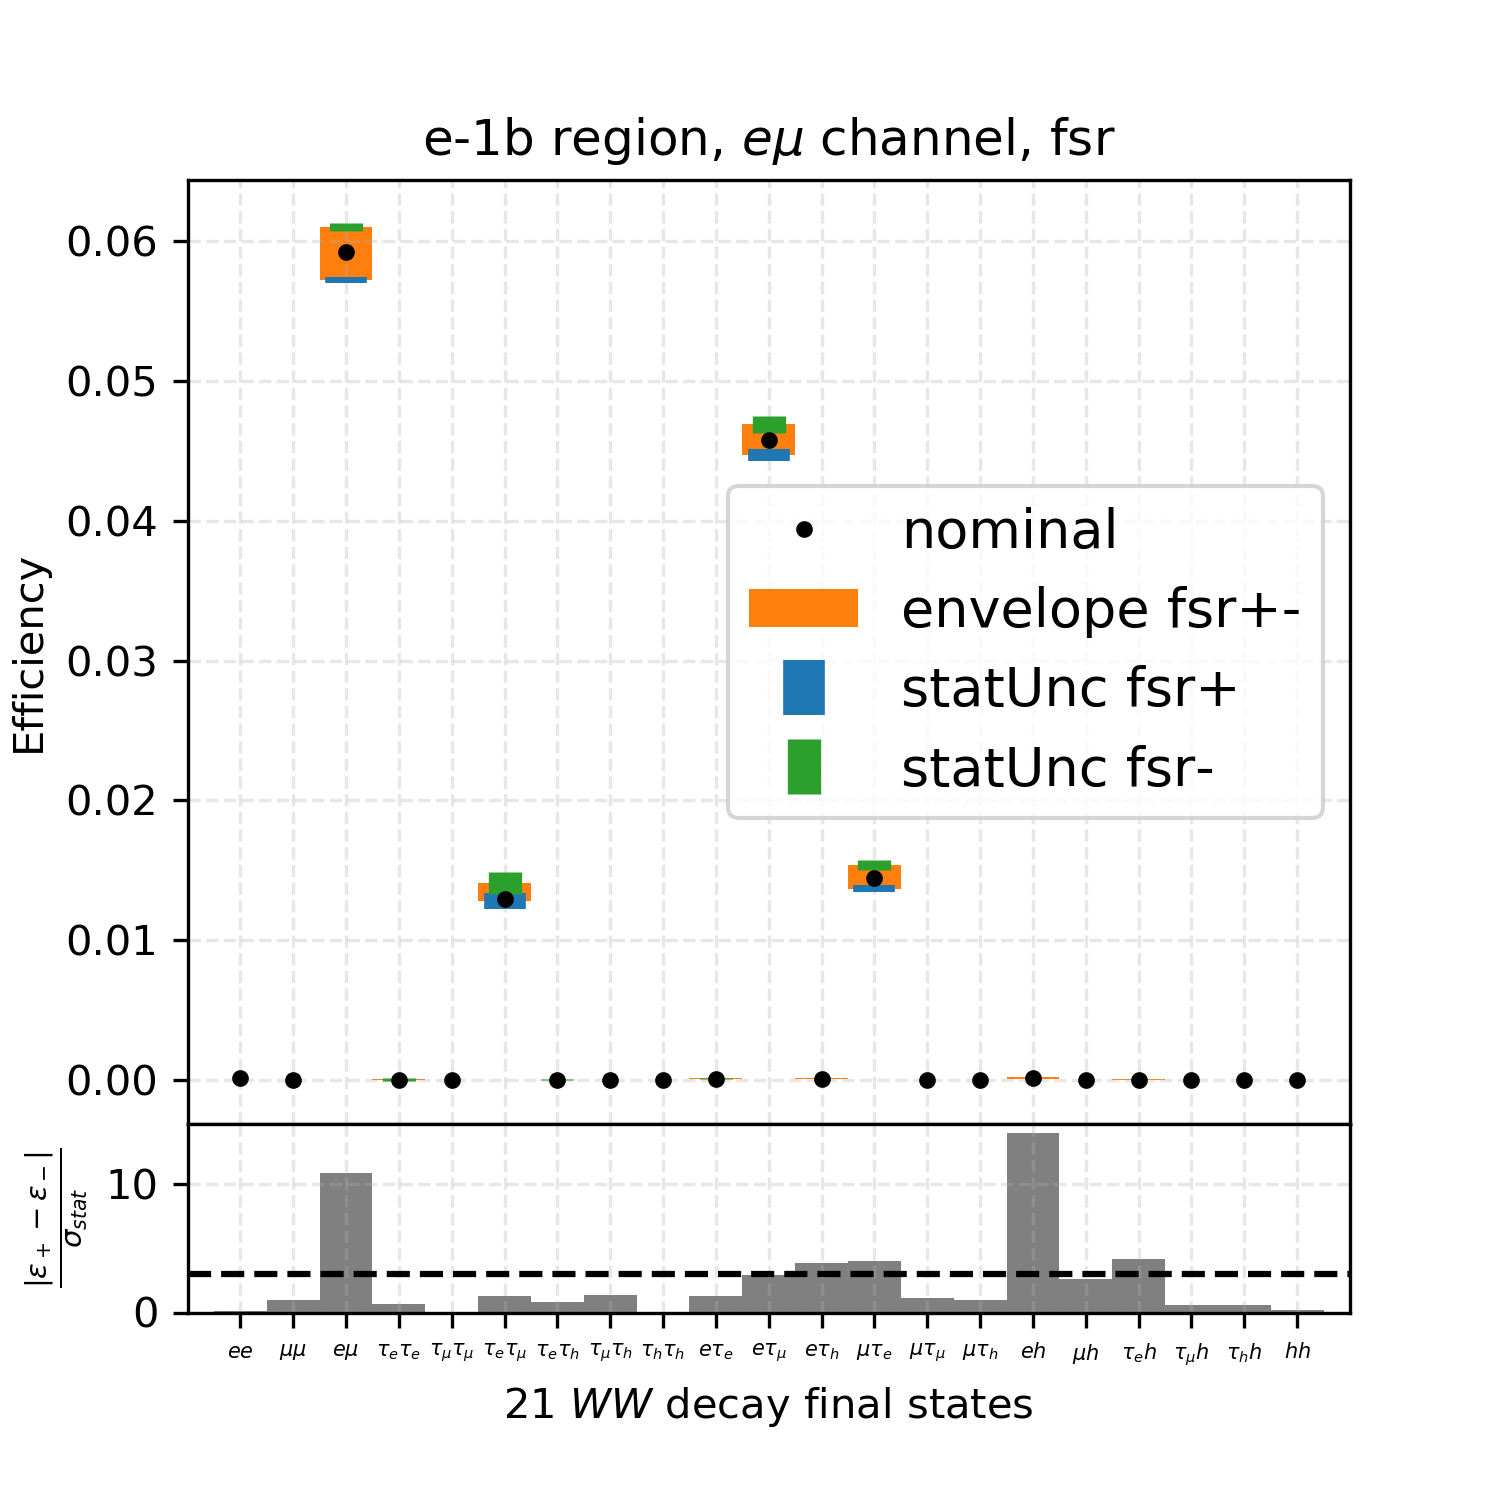
\includegraphics[width=0.24\textwidth]{chapters/Appendix/sectionTTSyst/figures/afterCorr/icata2_ch1_fsr.png}
    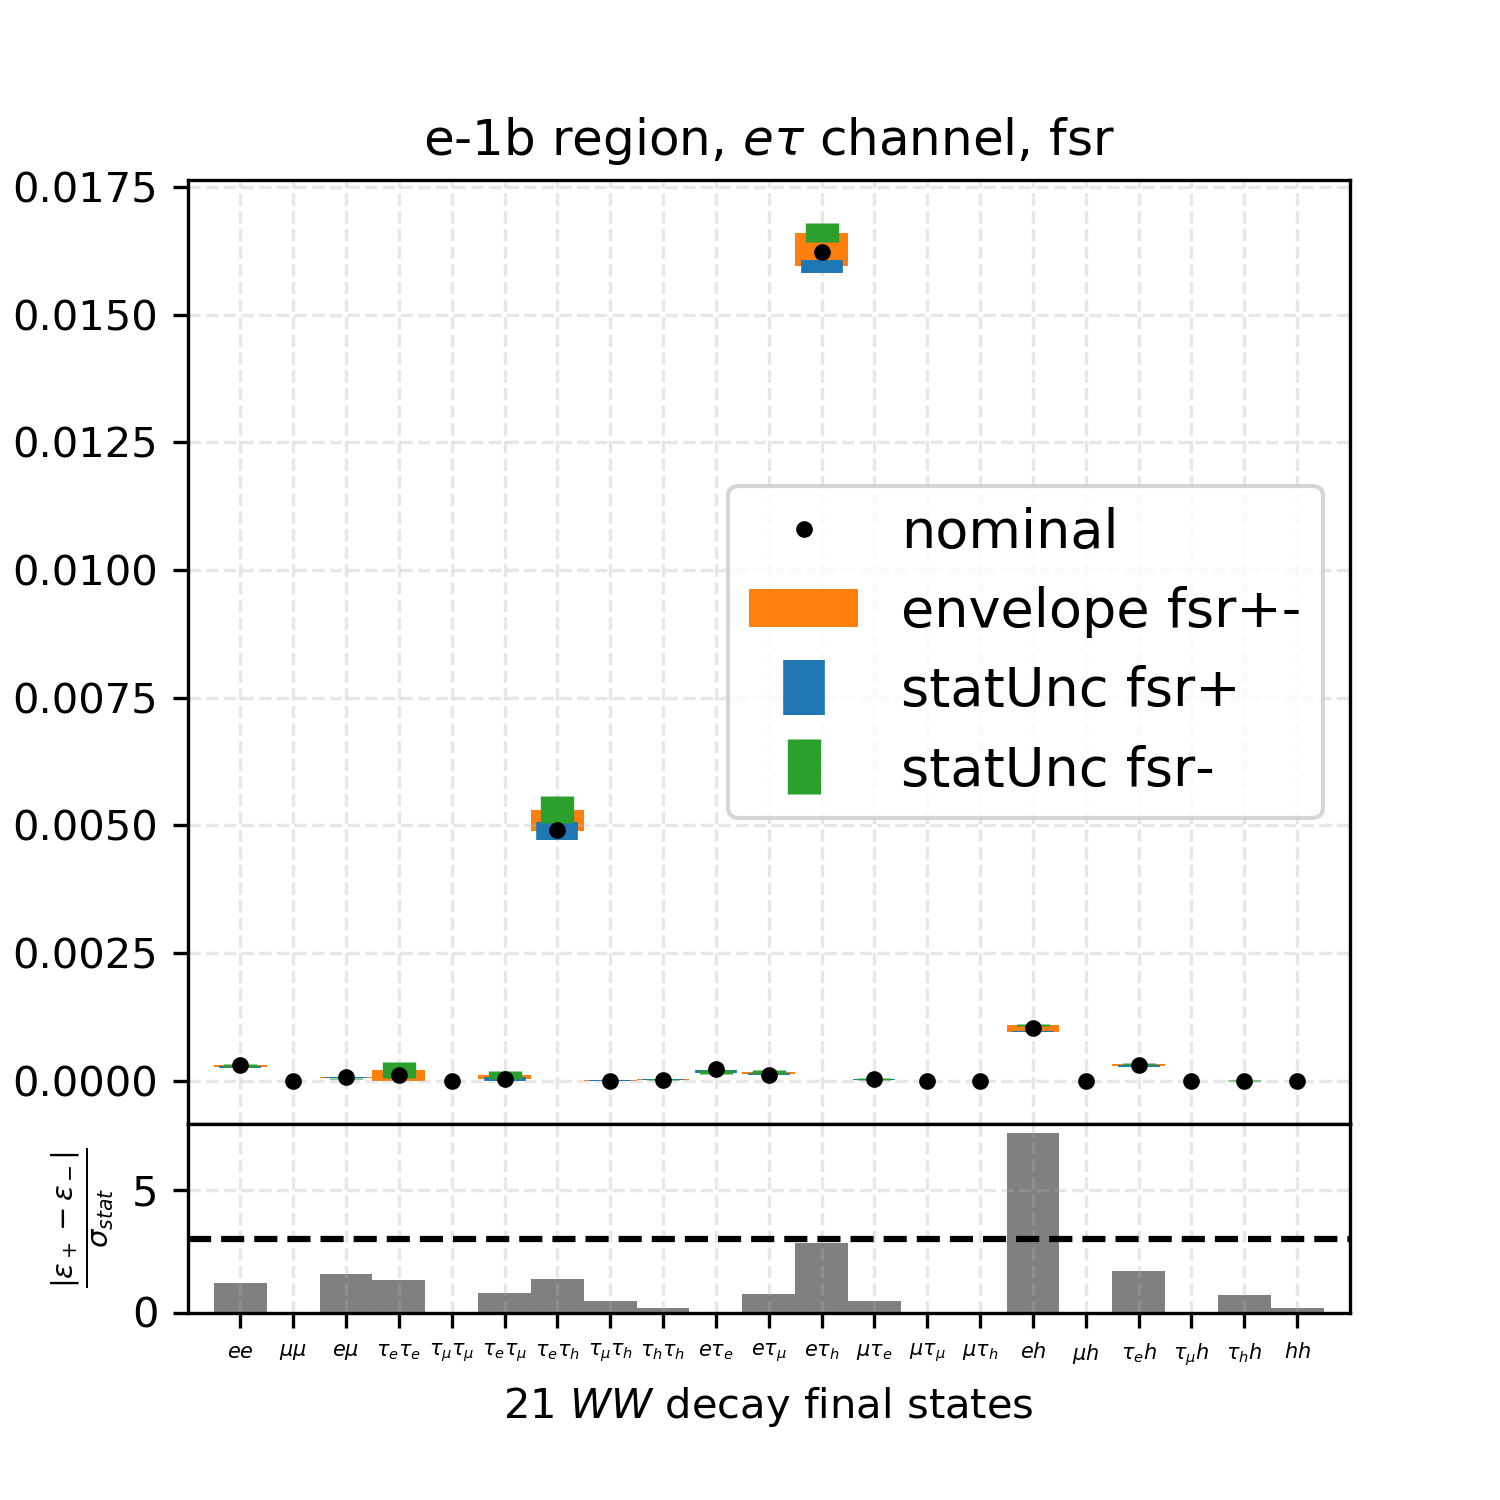
\includegraphics[width=0.24\textwidth]{chapters/Appendix/sectionTTSyst/figures/afterCorr/icata2_ch2_fsr.png}
    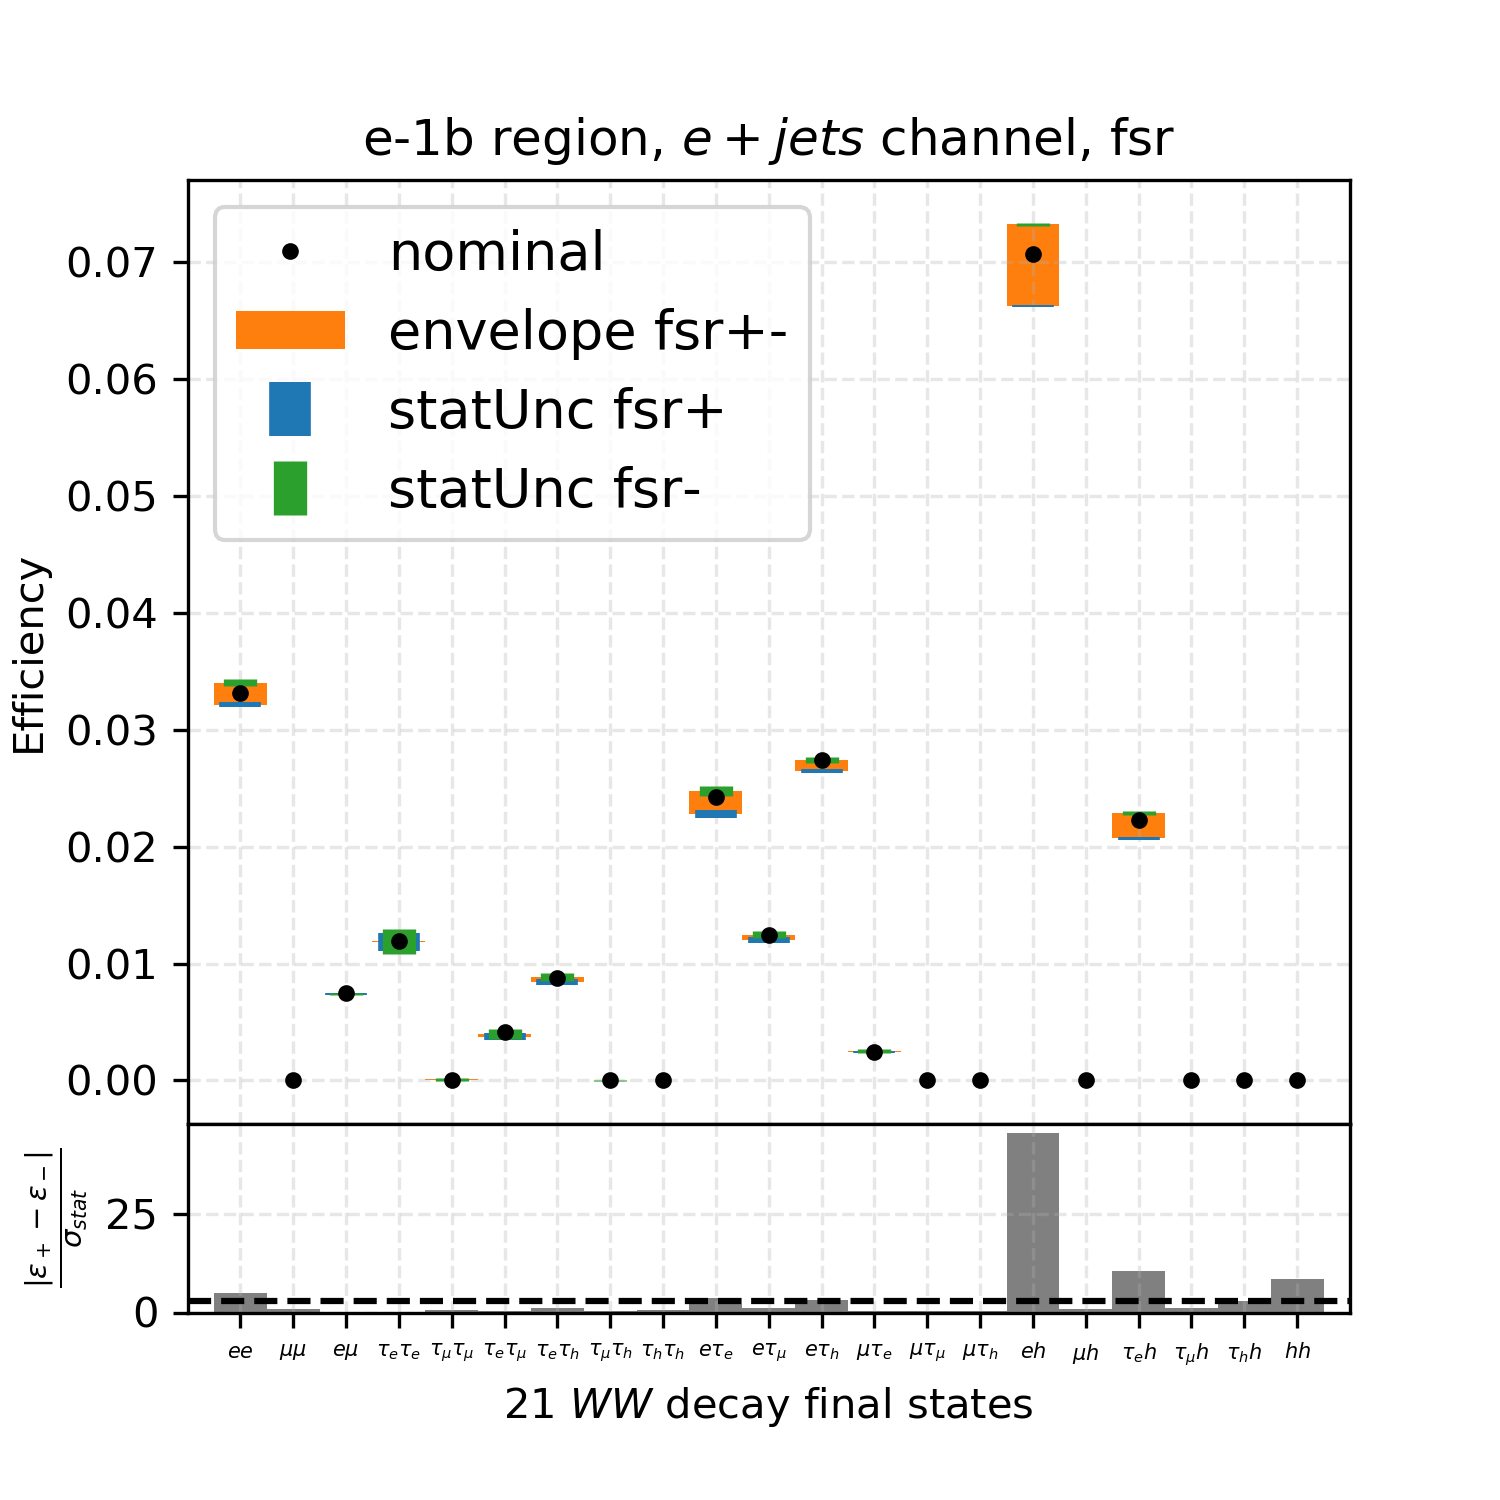
\includegraphics[width=0.24\textwidth]{chapters/Appendix/sectionTTSyst/figures/afterCorr/icata2_ch3_fsr.png}

    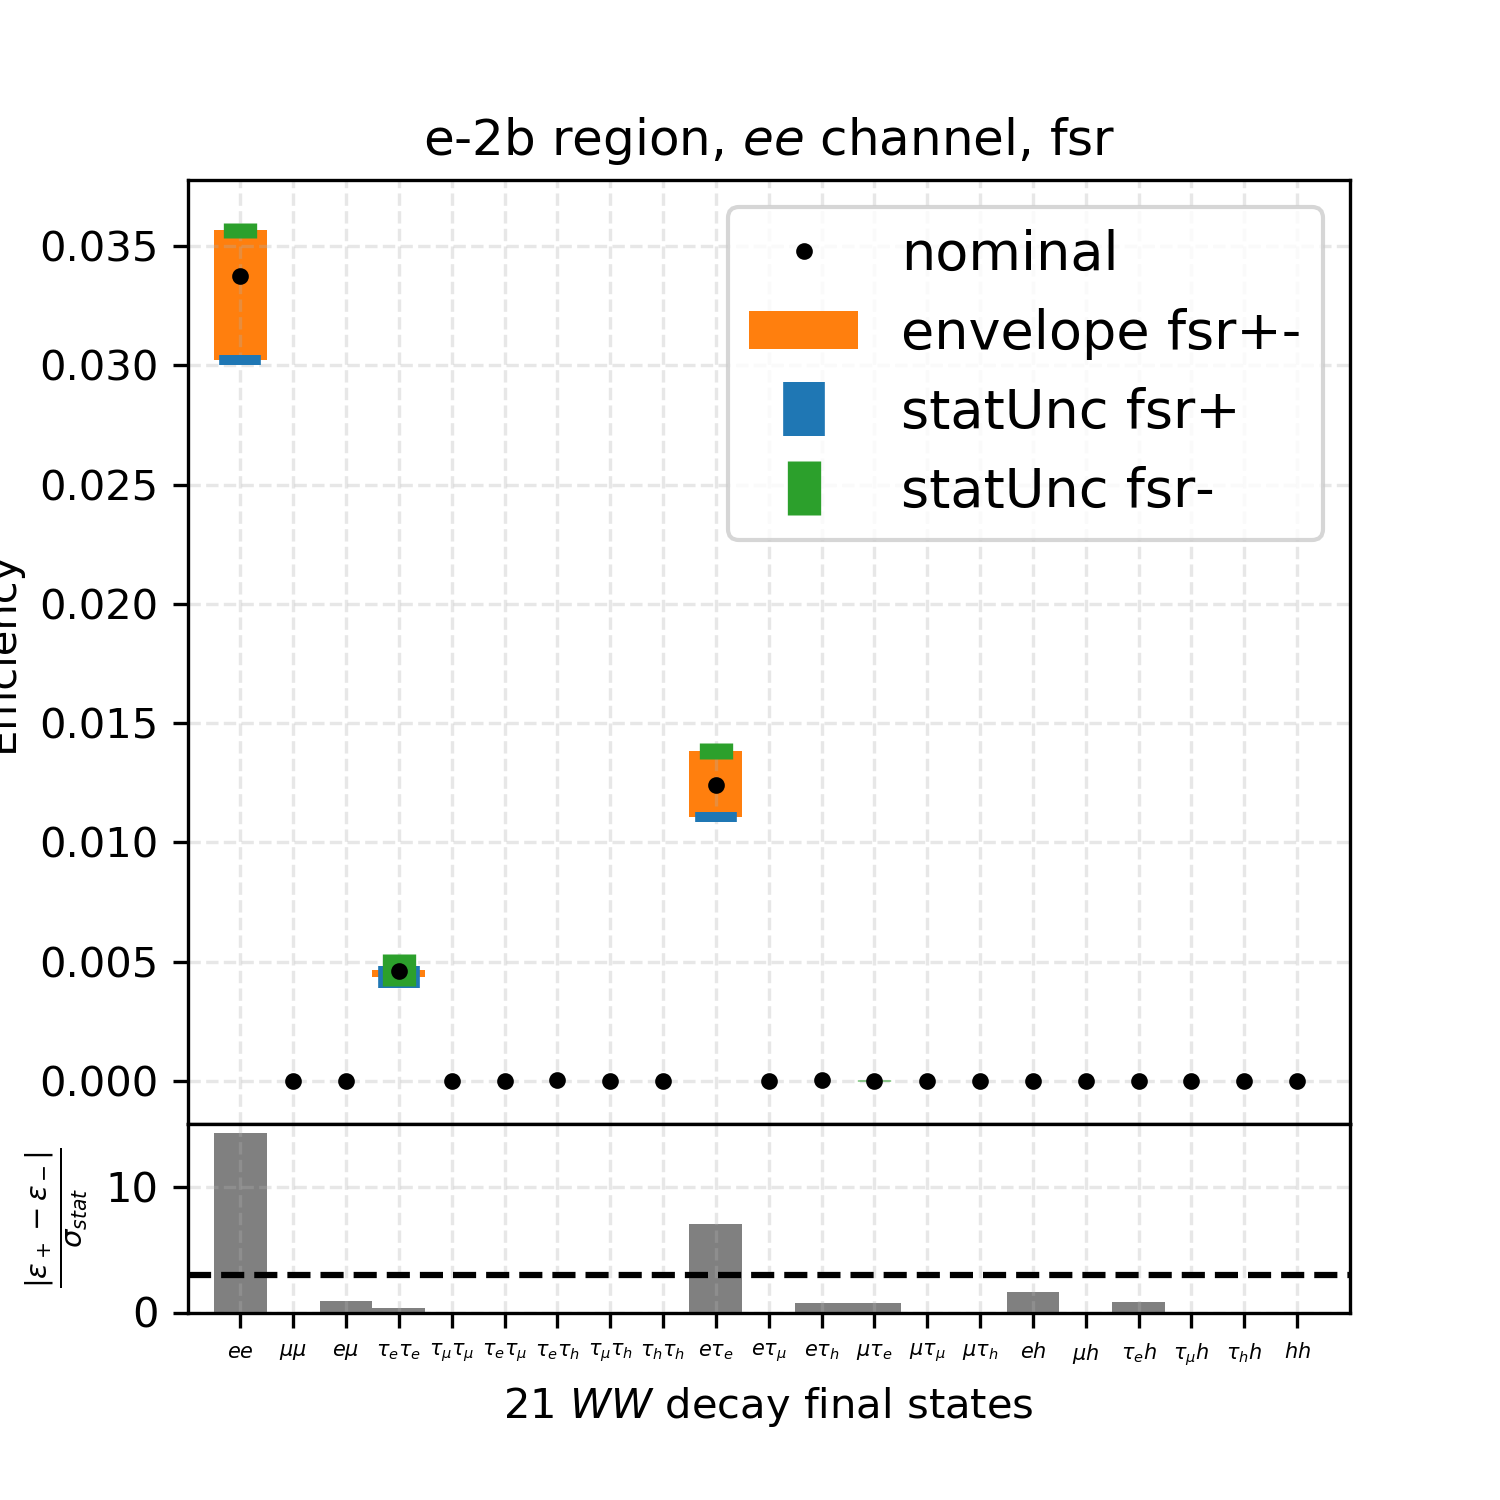
\includegraphics[width=0.24\textwidth]{chapters/Appendix/sectionTTSyst/figures/afterCorr/icata3_ch0_fsr.png}
    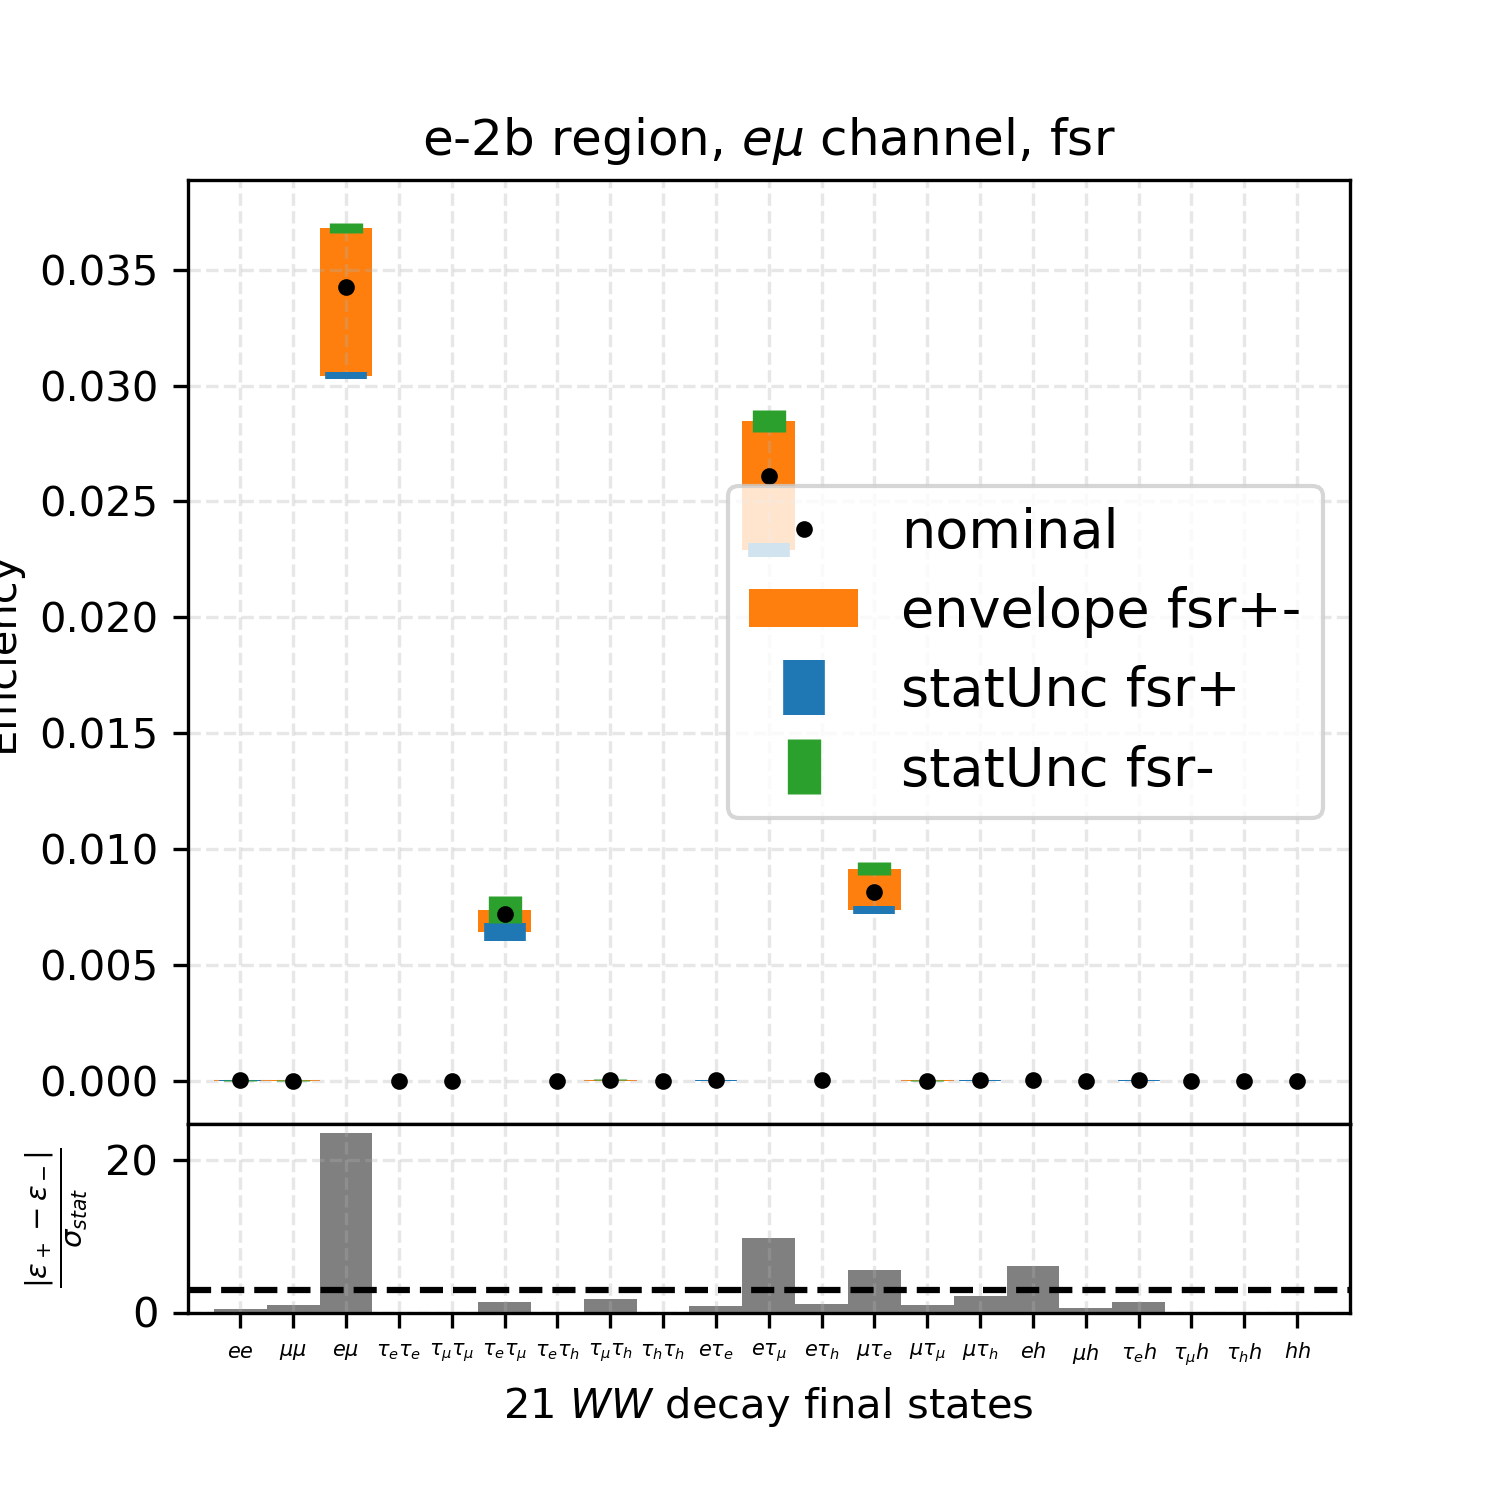
\includegraphics[width=0.24\textwidth]{chapters/Appendix/sectionTTSyst/figures/afterCorr/icata3_ch1_fsr.png}
    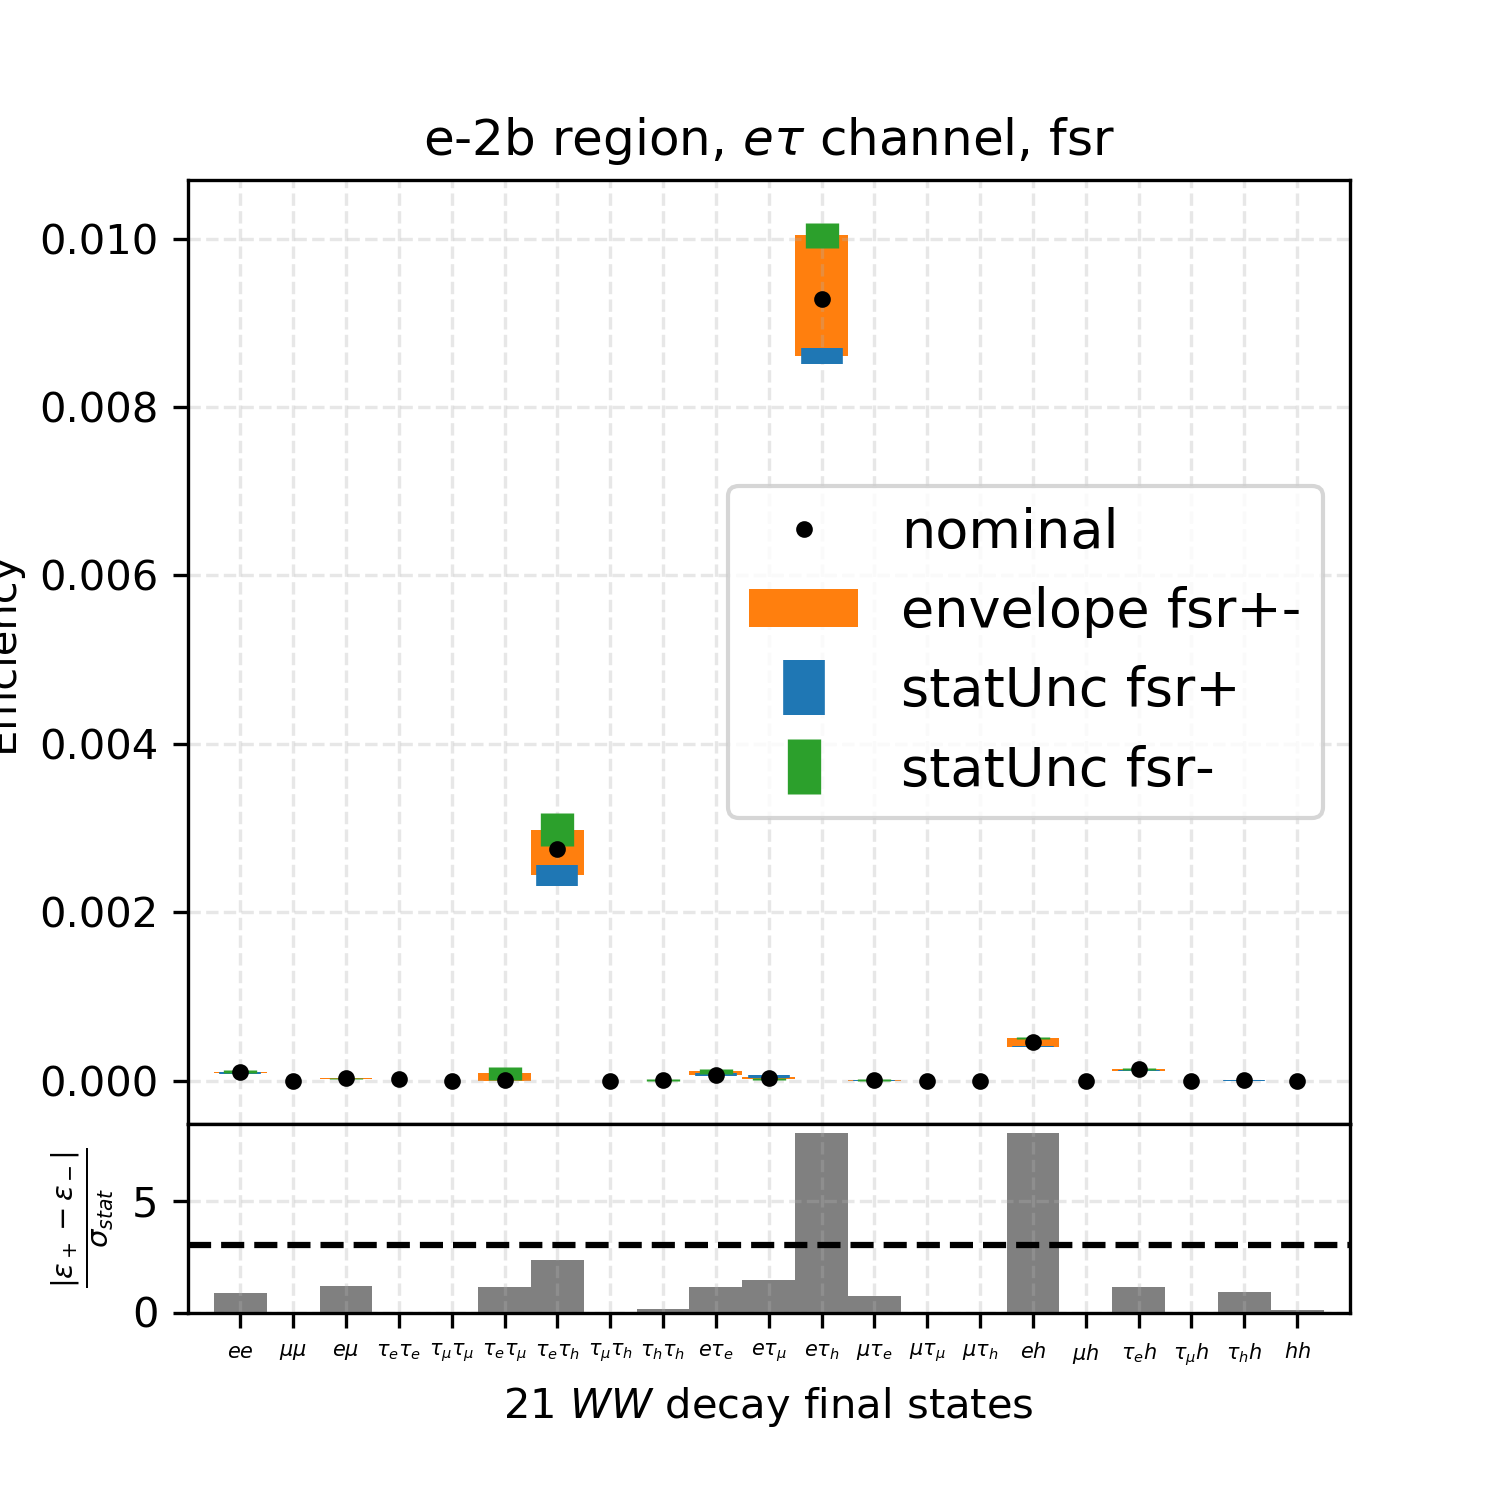
\includegraphics[width=0.24\textwidth]{chapters/Appendix/sectionTTSyst/figures/afterCorr/icata3_ch2_fsr.png}
    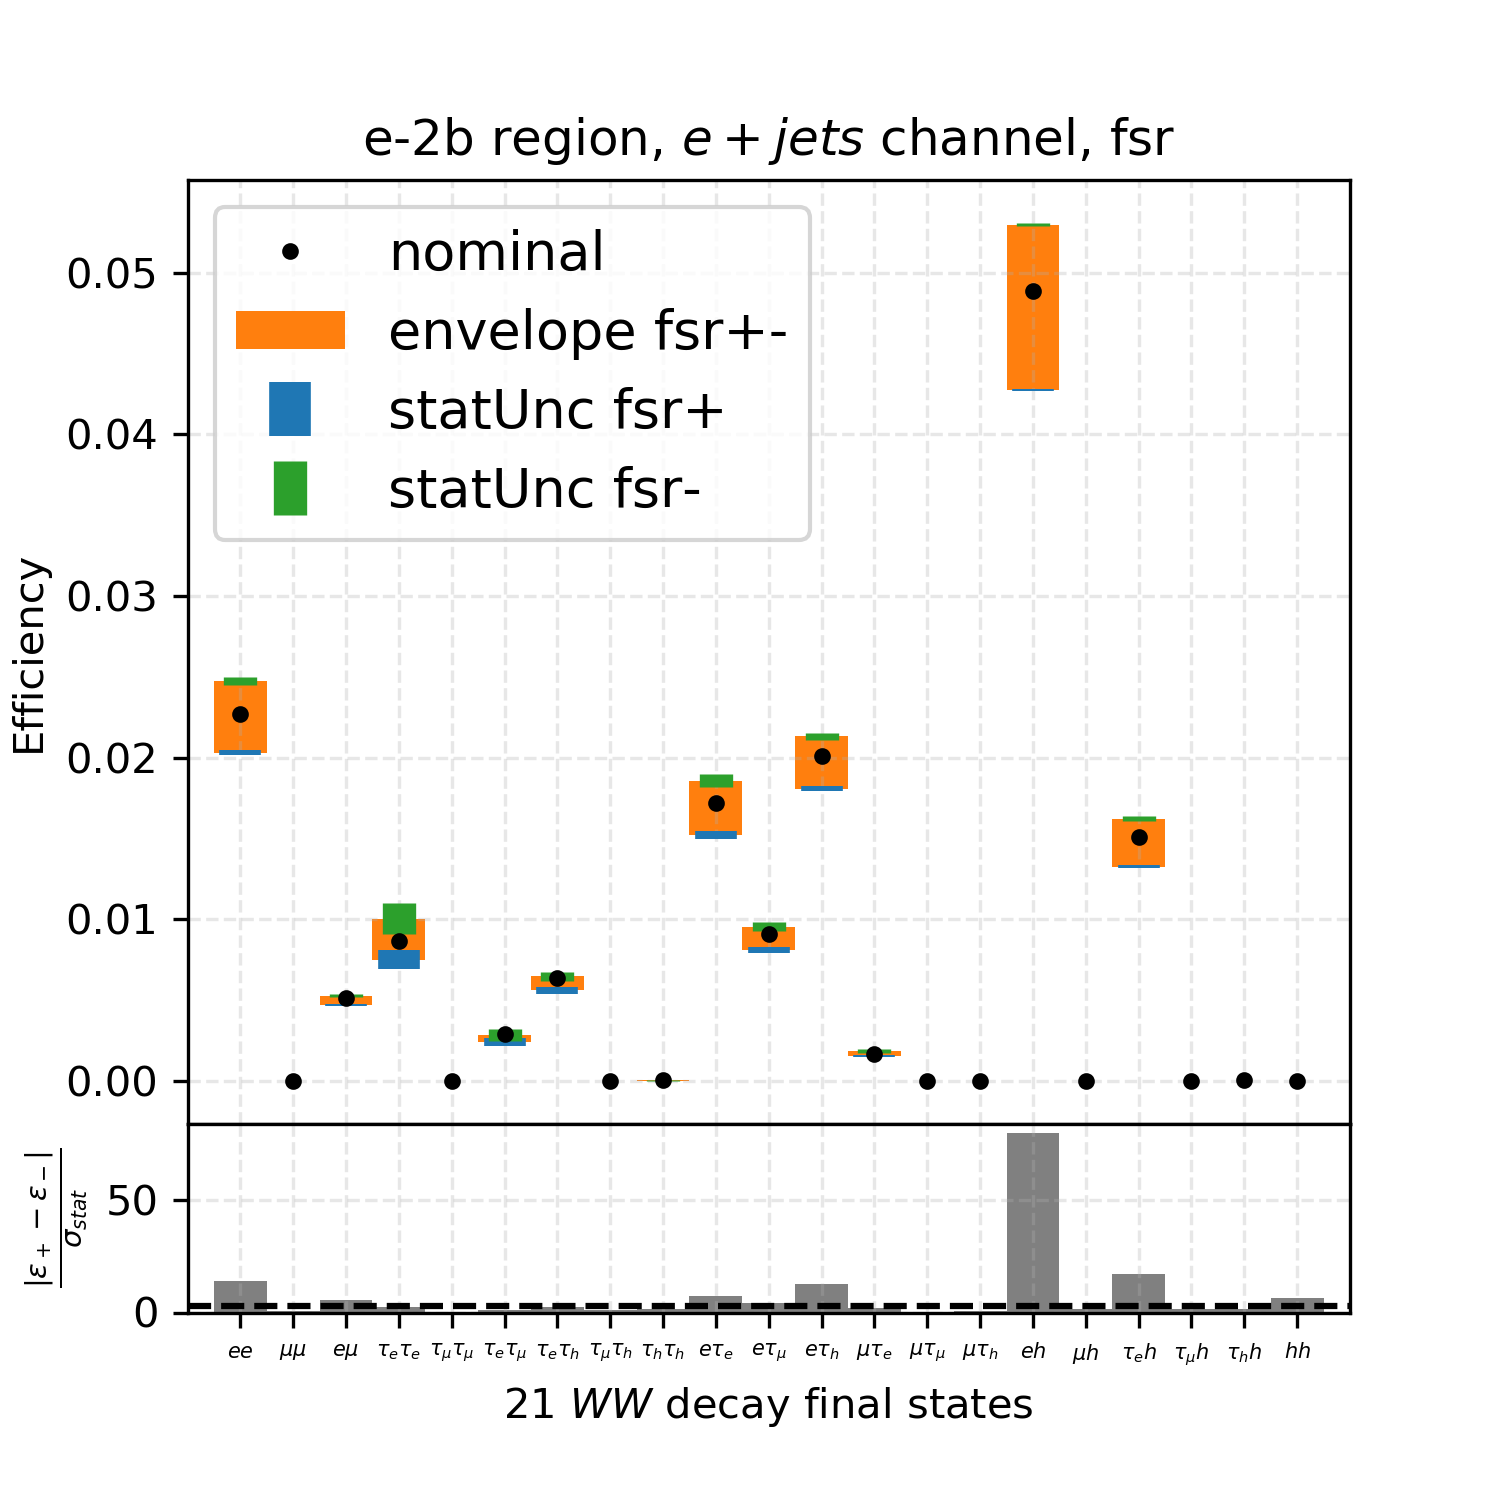
\includegraphics[width=0.24\textwidth]{chapters/Appendix/sectionTTSyst/figures/afterCorr/icata3_ch3_fsr.png}
    
    \caption{Reweight $\tau_h$ and $j \to \tau_h$ efficiencies in the dedicated FSR, ISF, MEPS, UE ttbar samples}
    \label{fig:appendix:reweighttt:effAfterCorrFSR}
\end{figure}



\begin{figure}
    \centering
    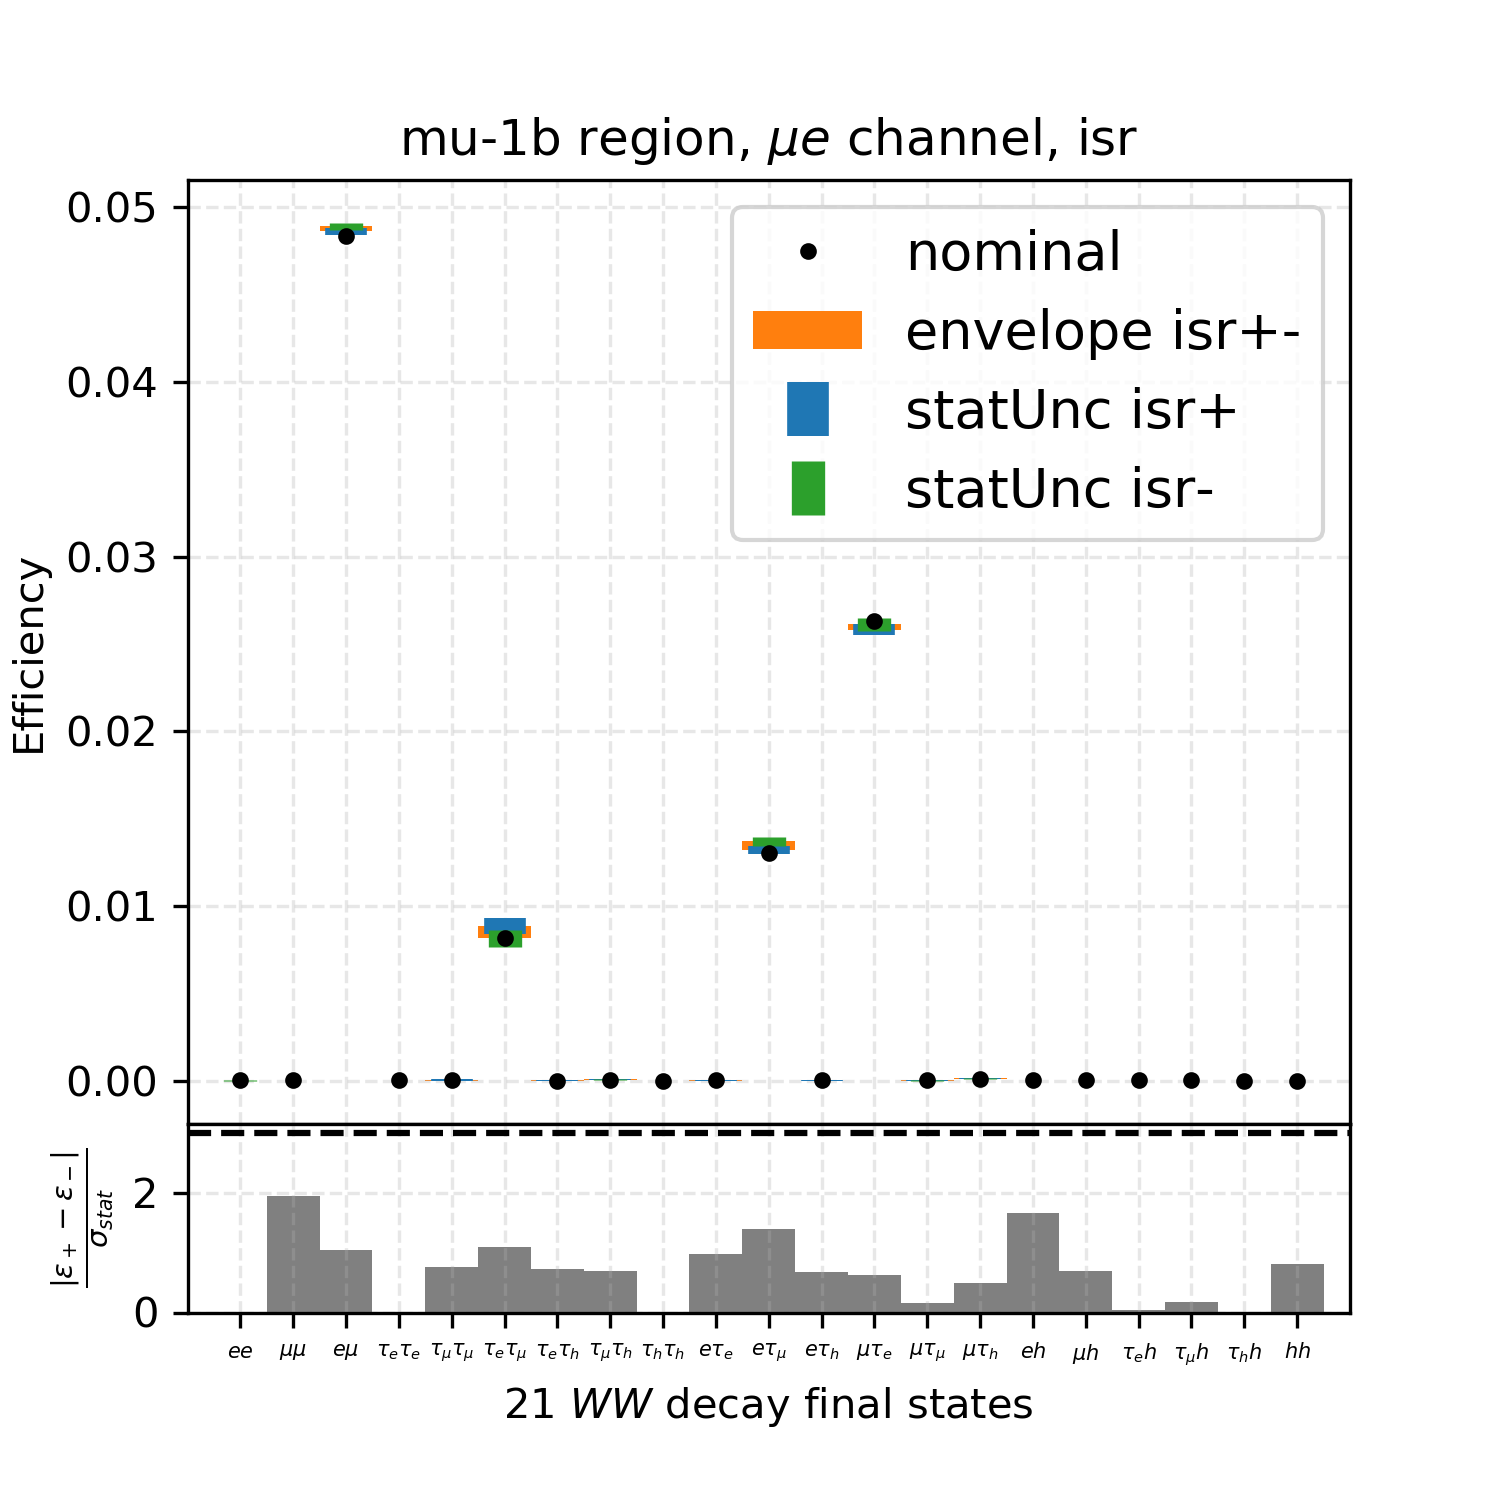
\includegraphics[width=0.24\textwidth]{chapters/Appendix/sectionTTSyst/figures/afterCorr/icata0_ch0_isr.png}
    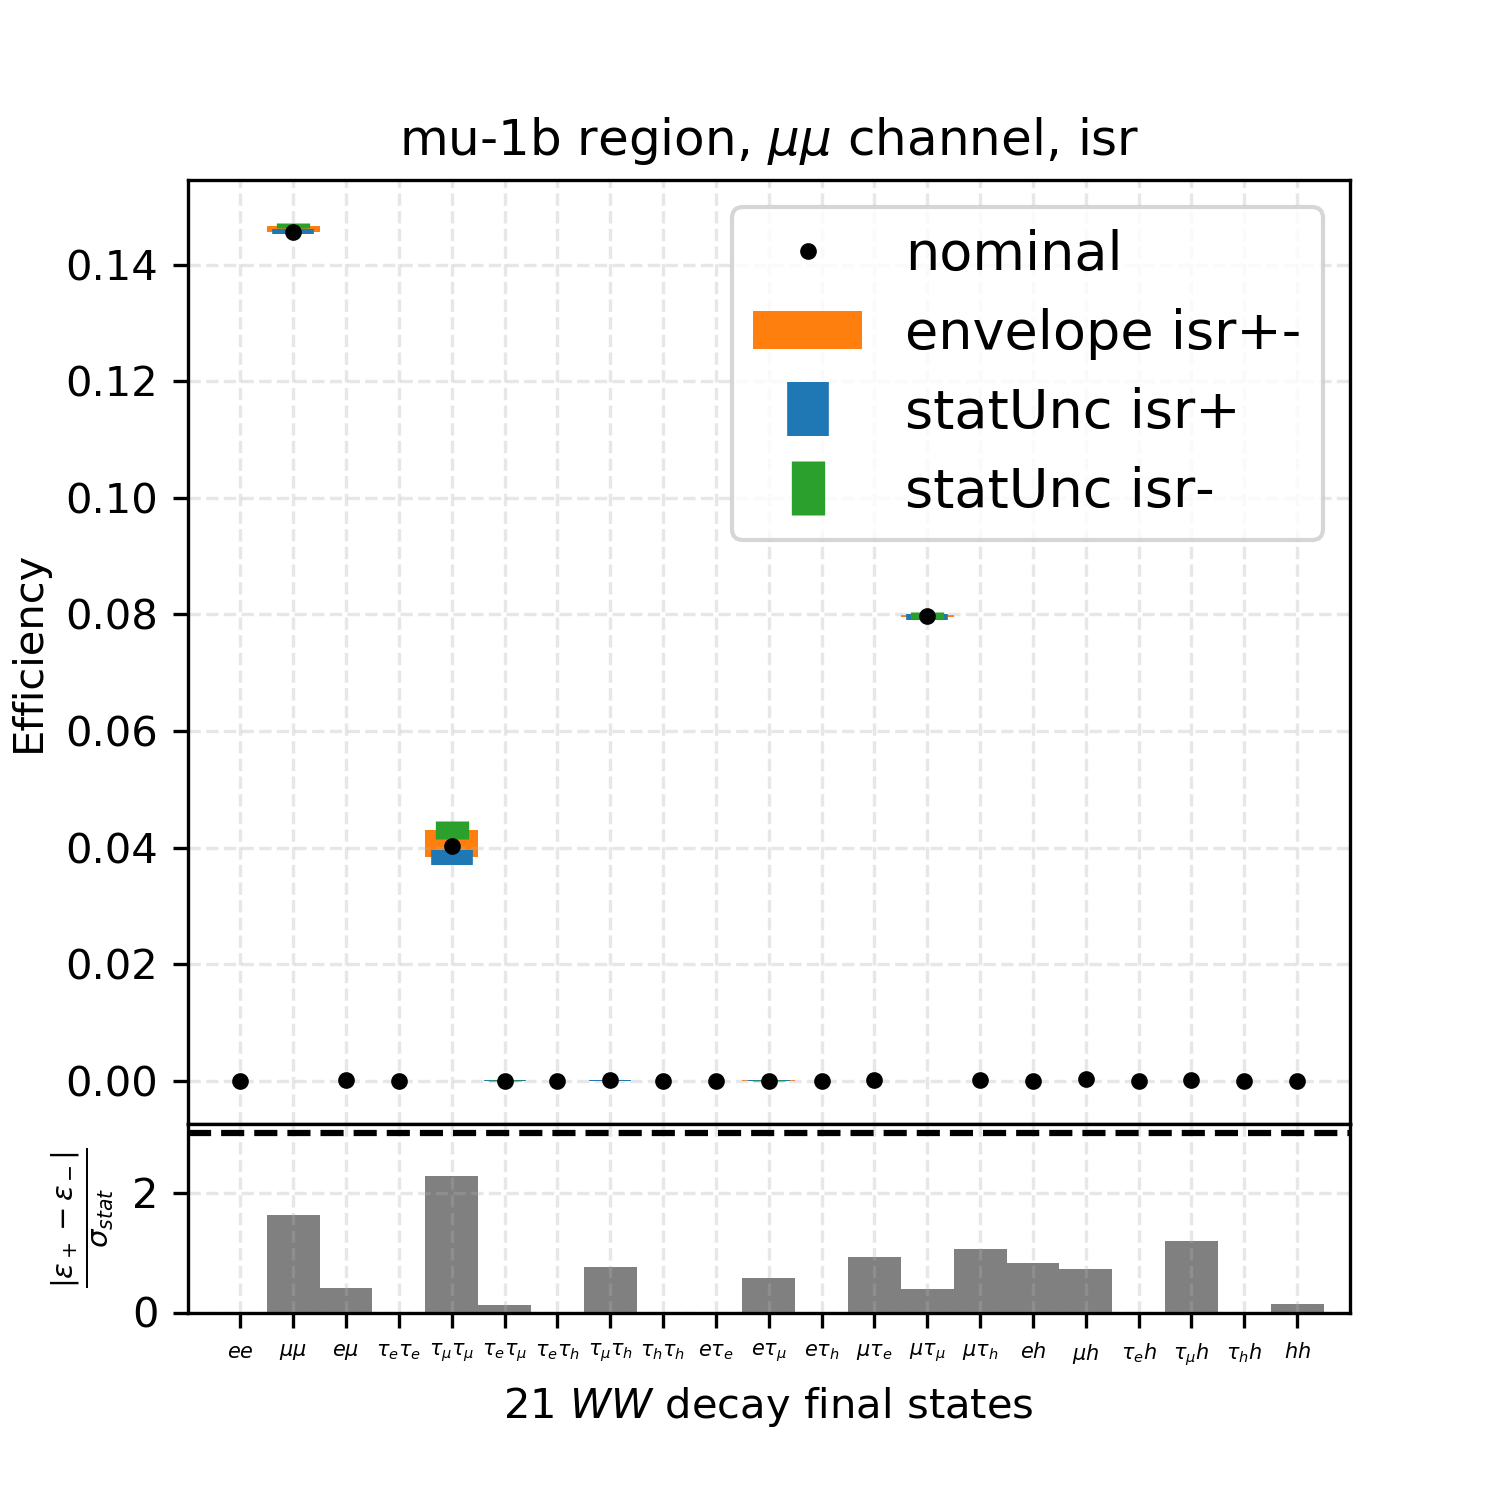
\includegraphics[width=0.24\textwidth]{chapters/Appendix/sectionTTSyst/figures/afterCorr/icata0_ch1_isr.png}
    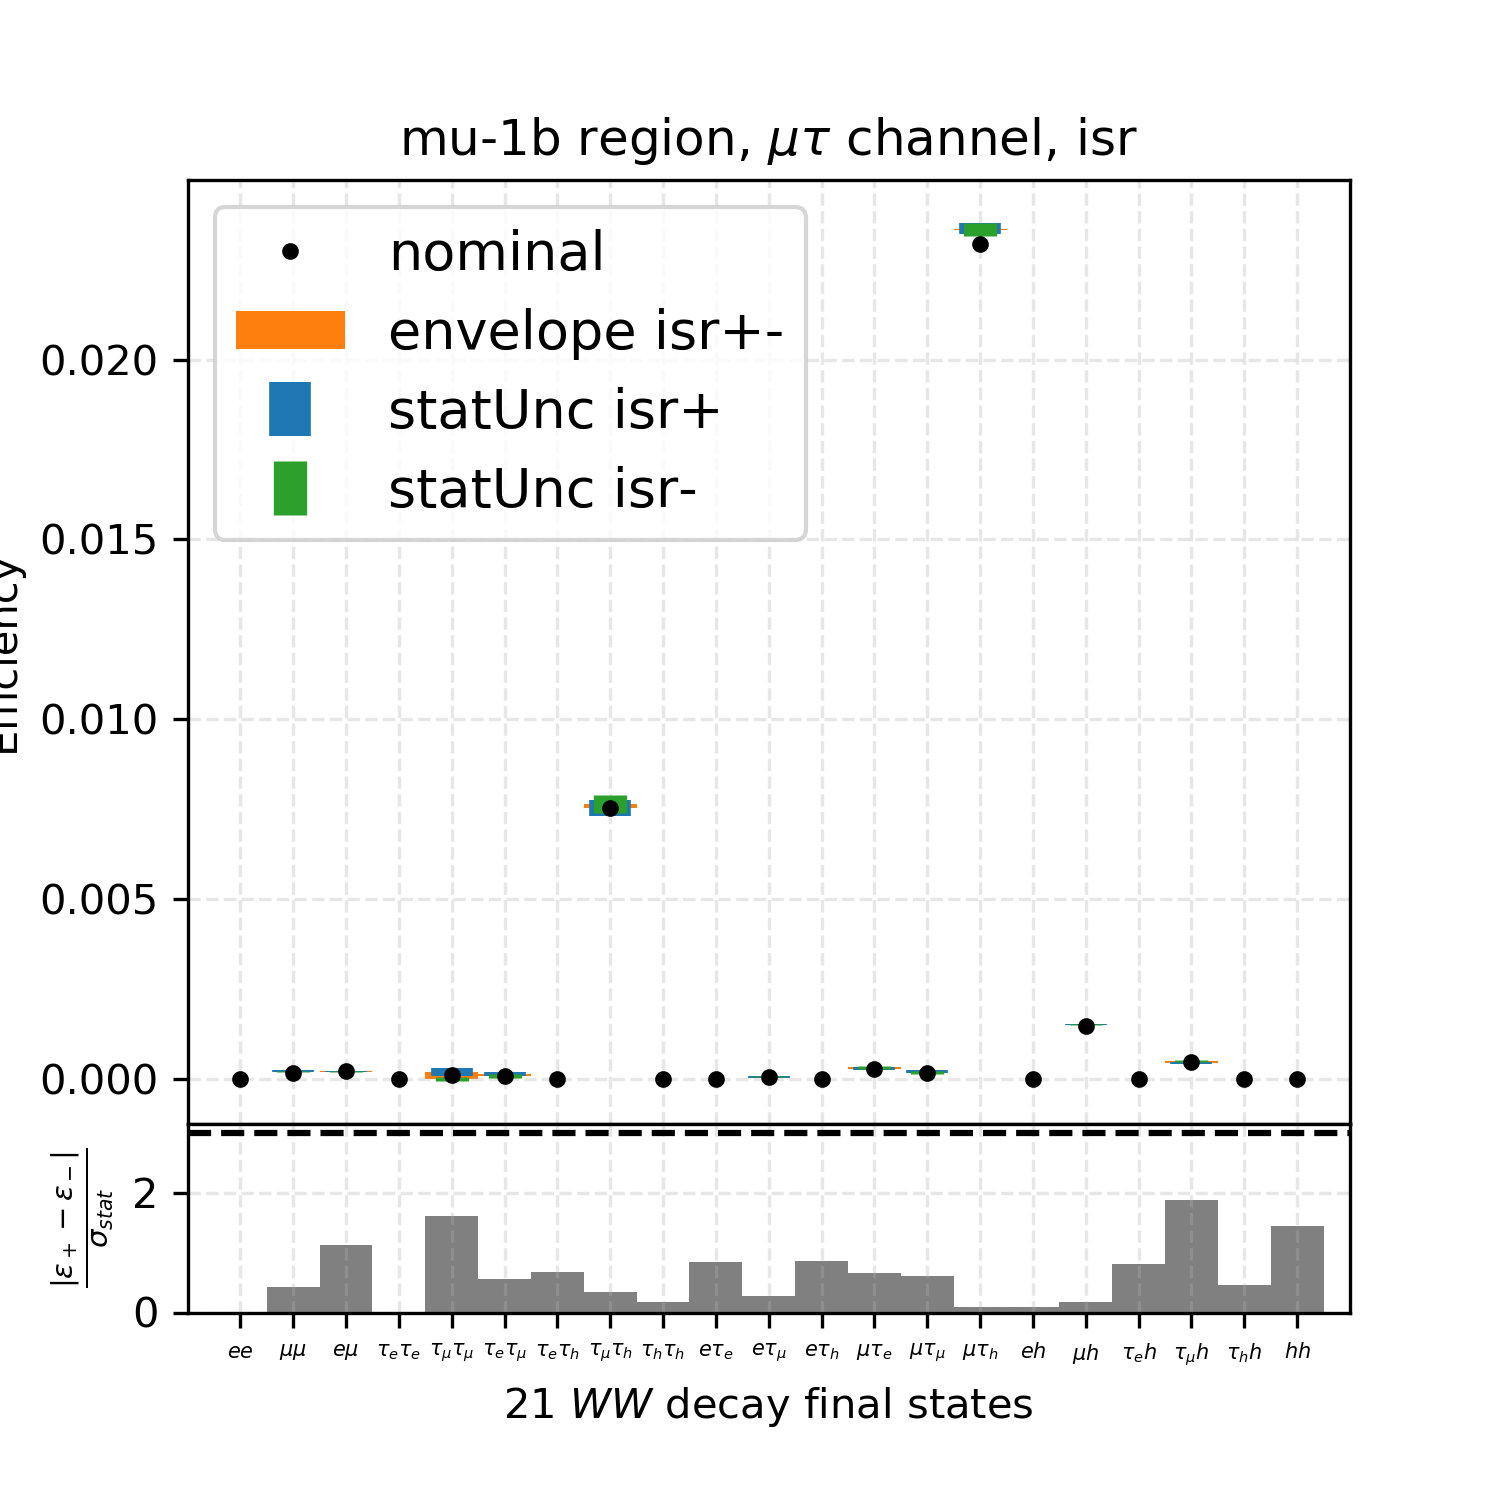
\includegraphics[width=0.24\textwidth]{chapters/Appendix/sectionTTSyst/figures/afterCorr/icata0_ch2_isr.png}
    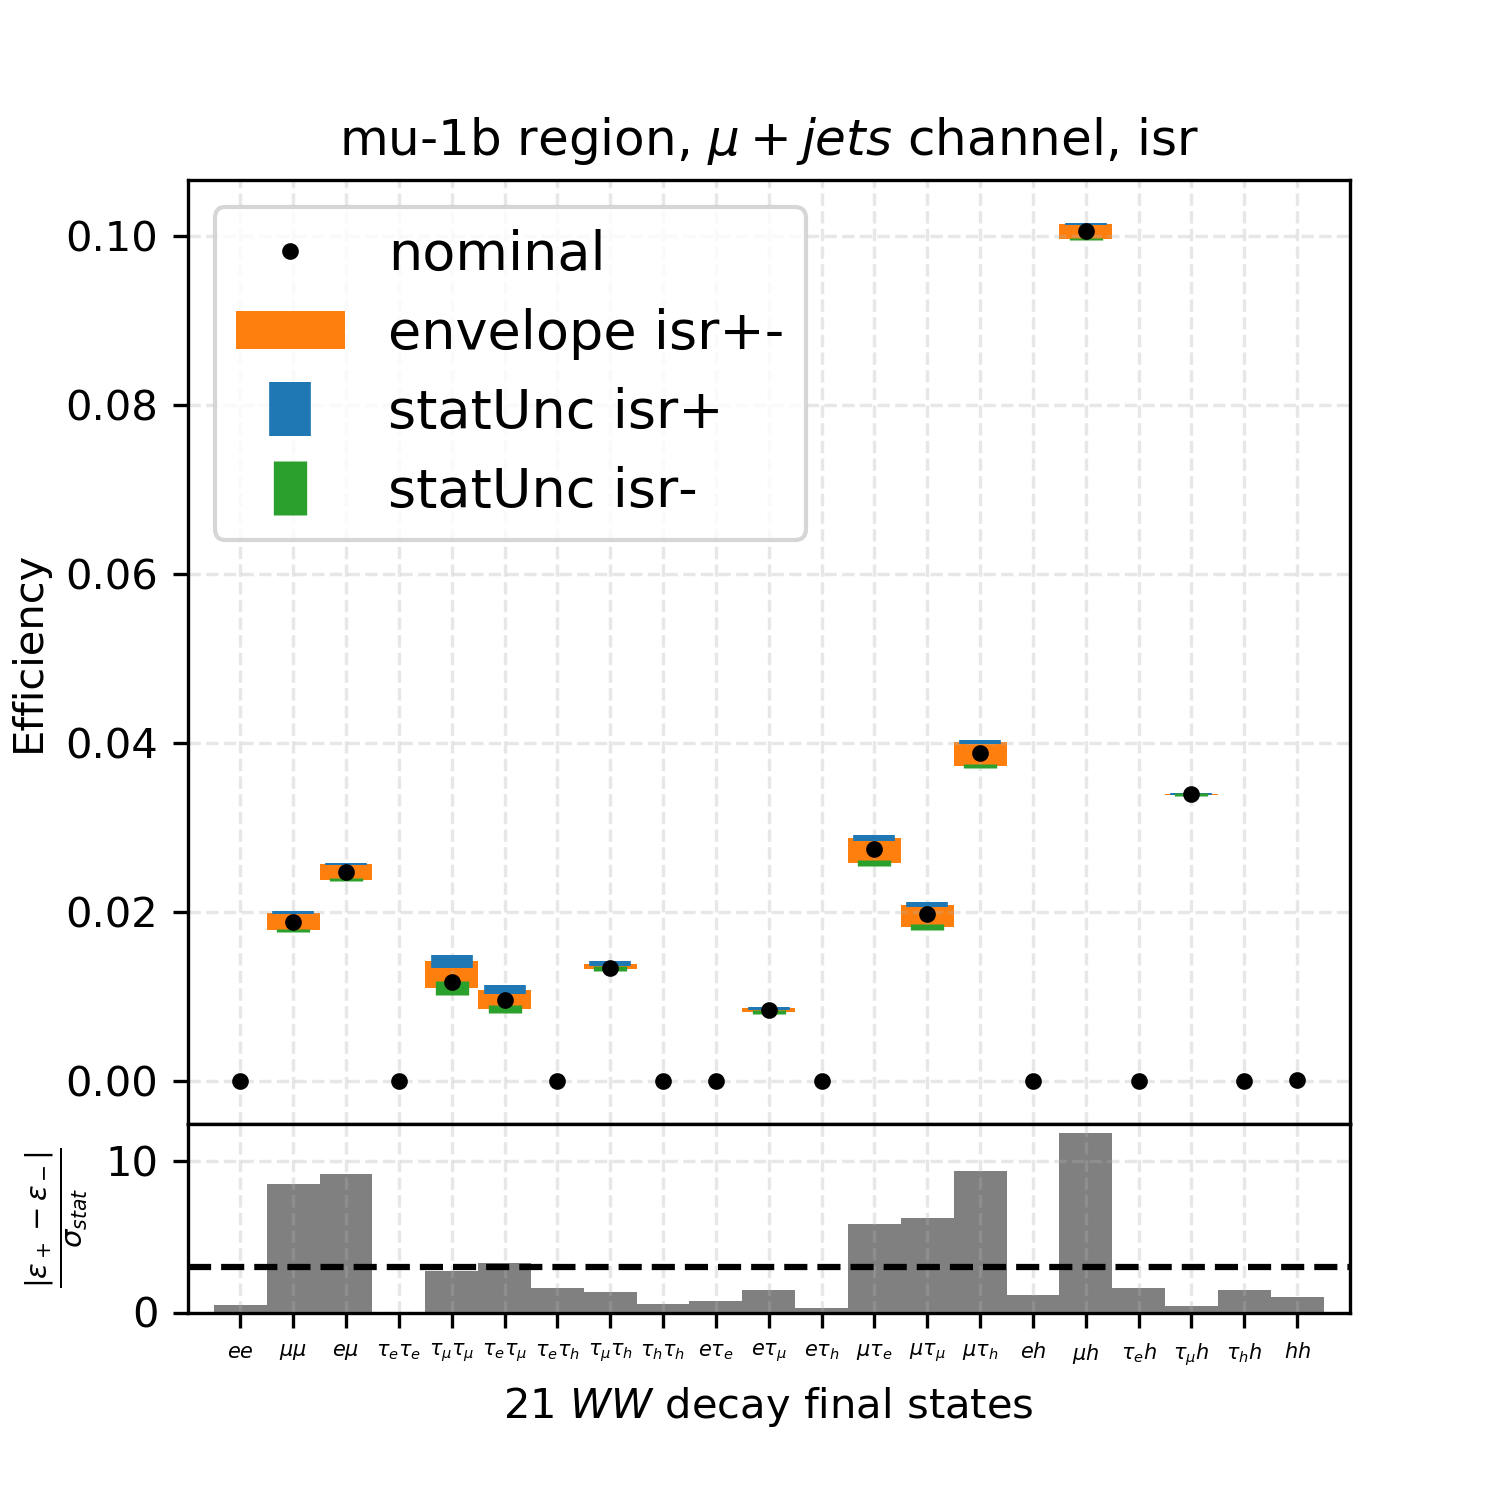
\includegraphics[width=0.24\textwidth]{chapters/Appendix/sectionTTSyst/figures/afterCorr/icata0_ch3_isr.png}

    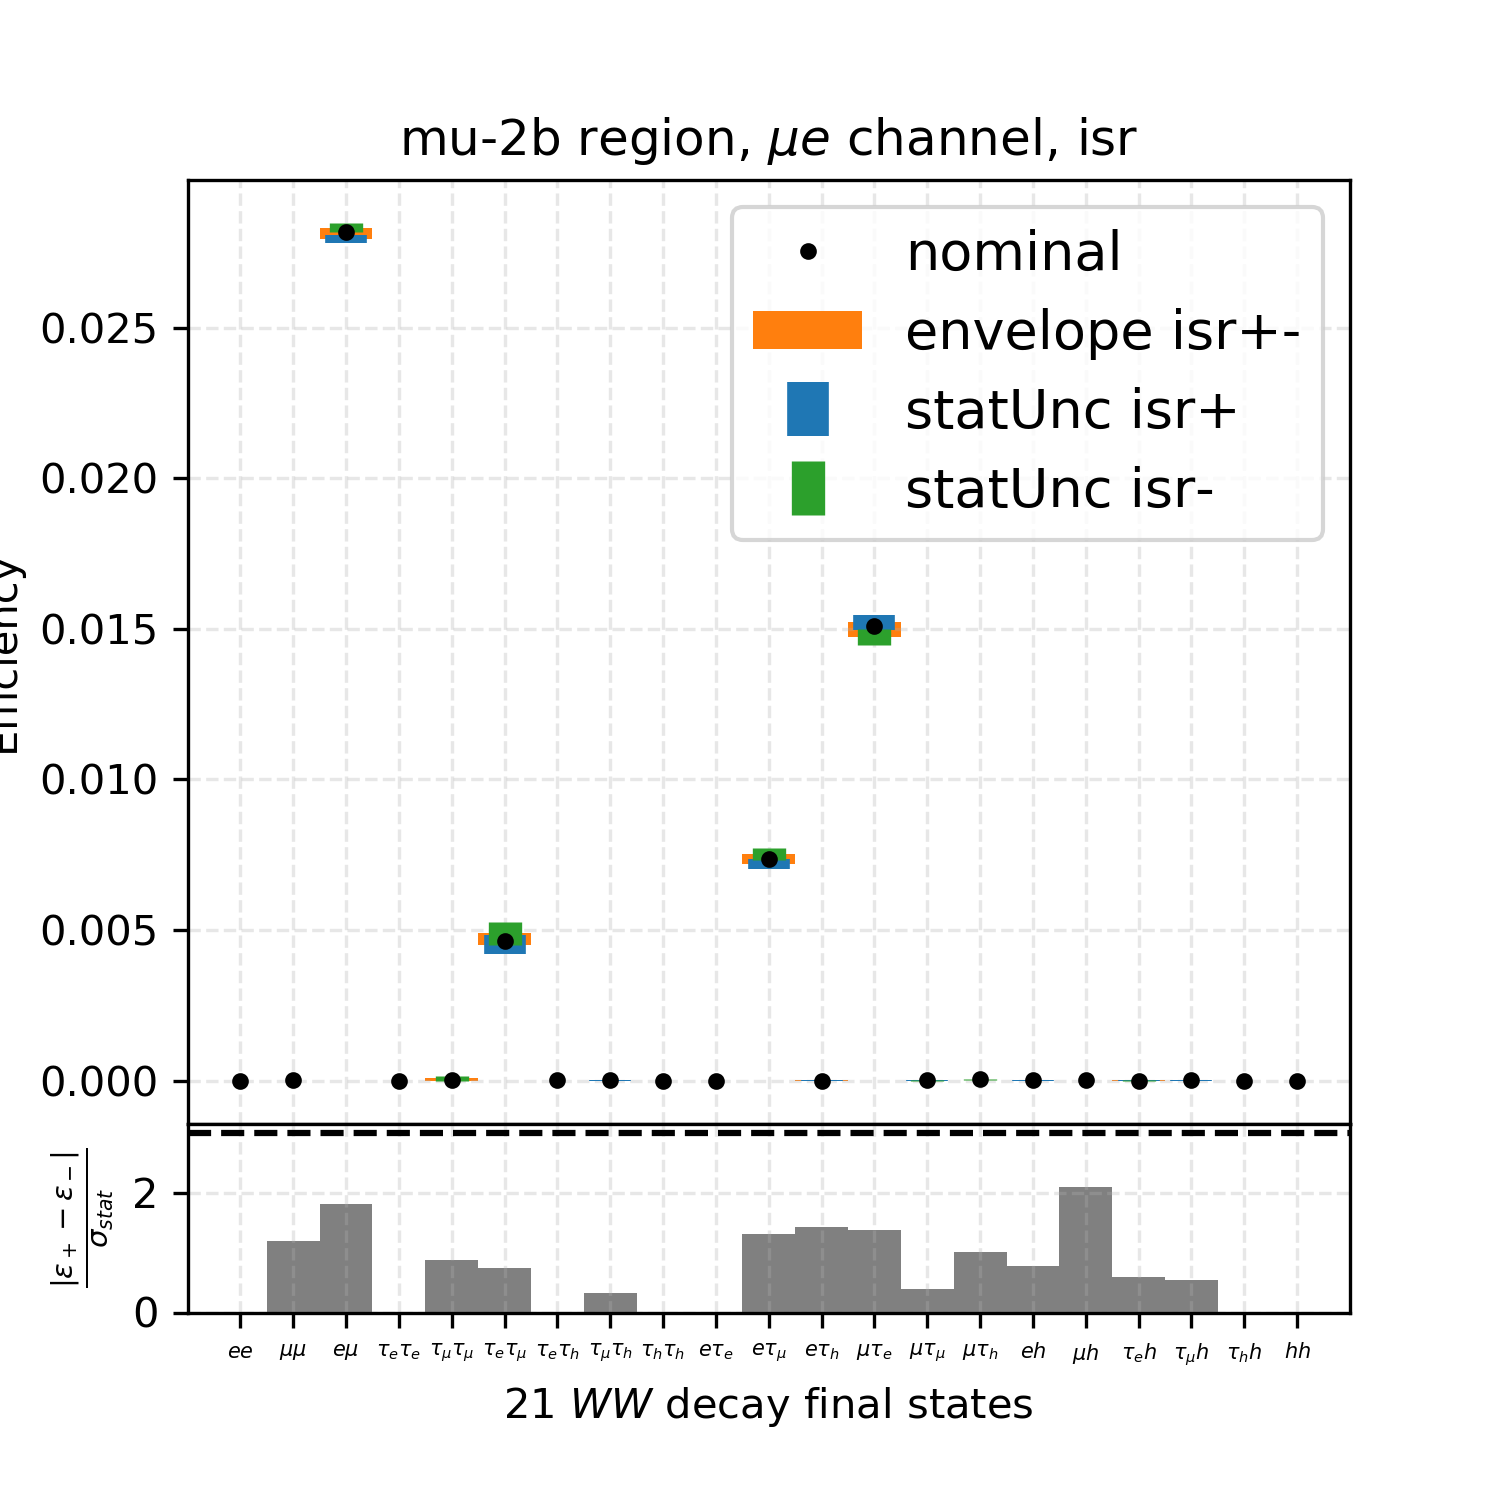
\includegraphics[width=0.24\textwidth]{chapters/Appendix/sectionTTSyst/figures/afterCorr/icata1_ch0_isr.png}
    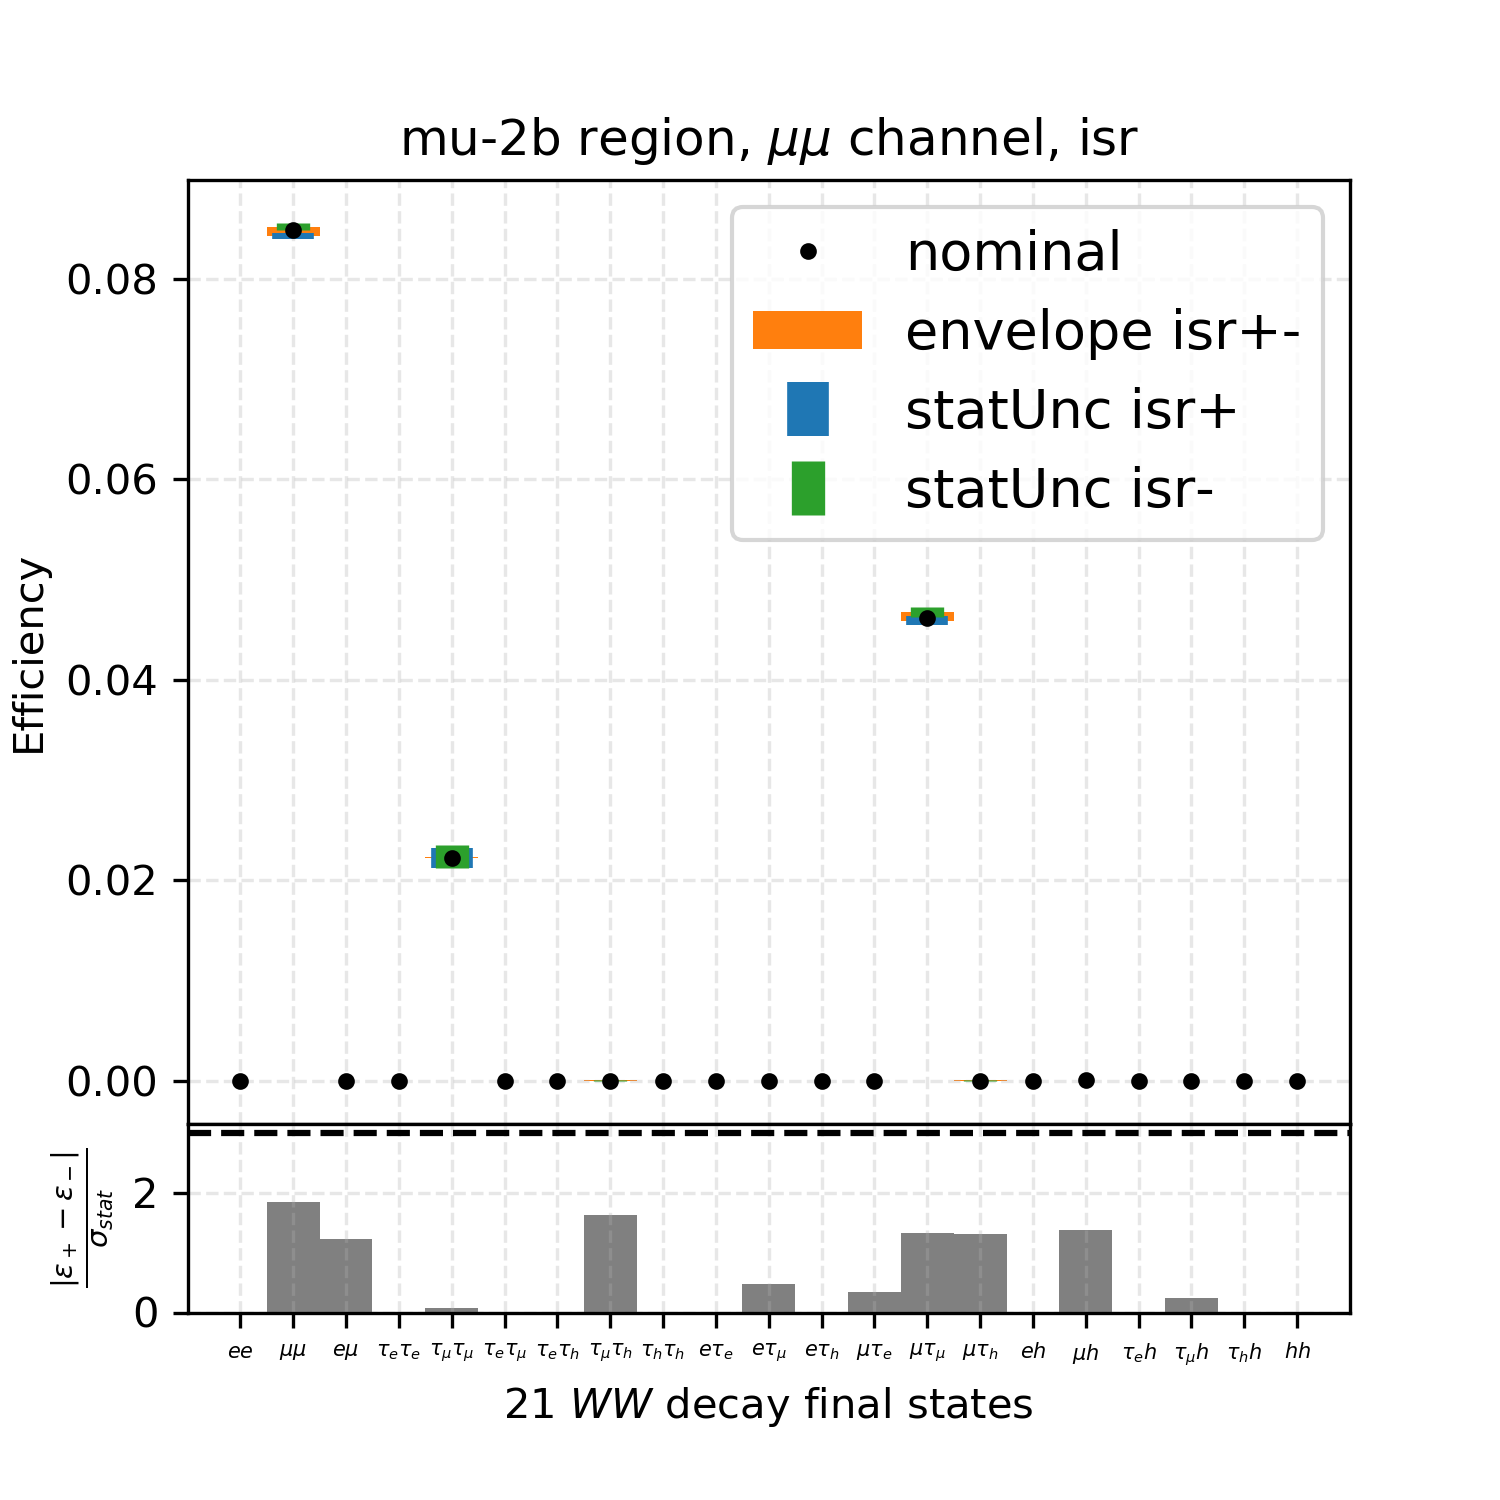
\includegraphics[width=0.24\textwidth]{chapters/Appendix/sectionTTSyst/figures/afterCorr/icata1_ch1_isr.png}
    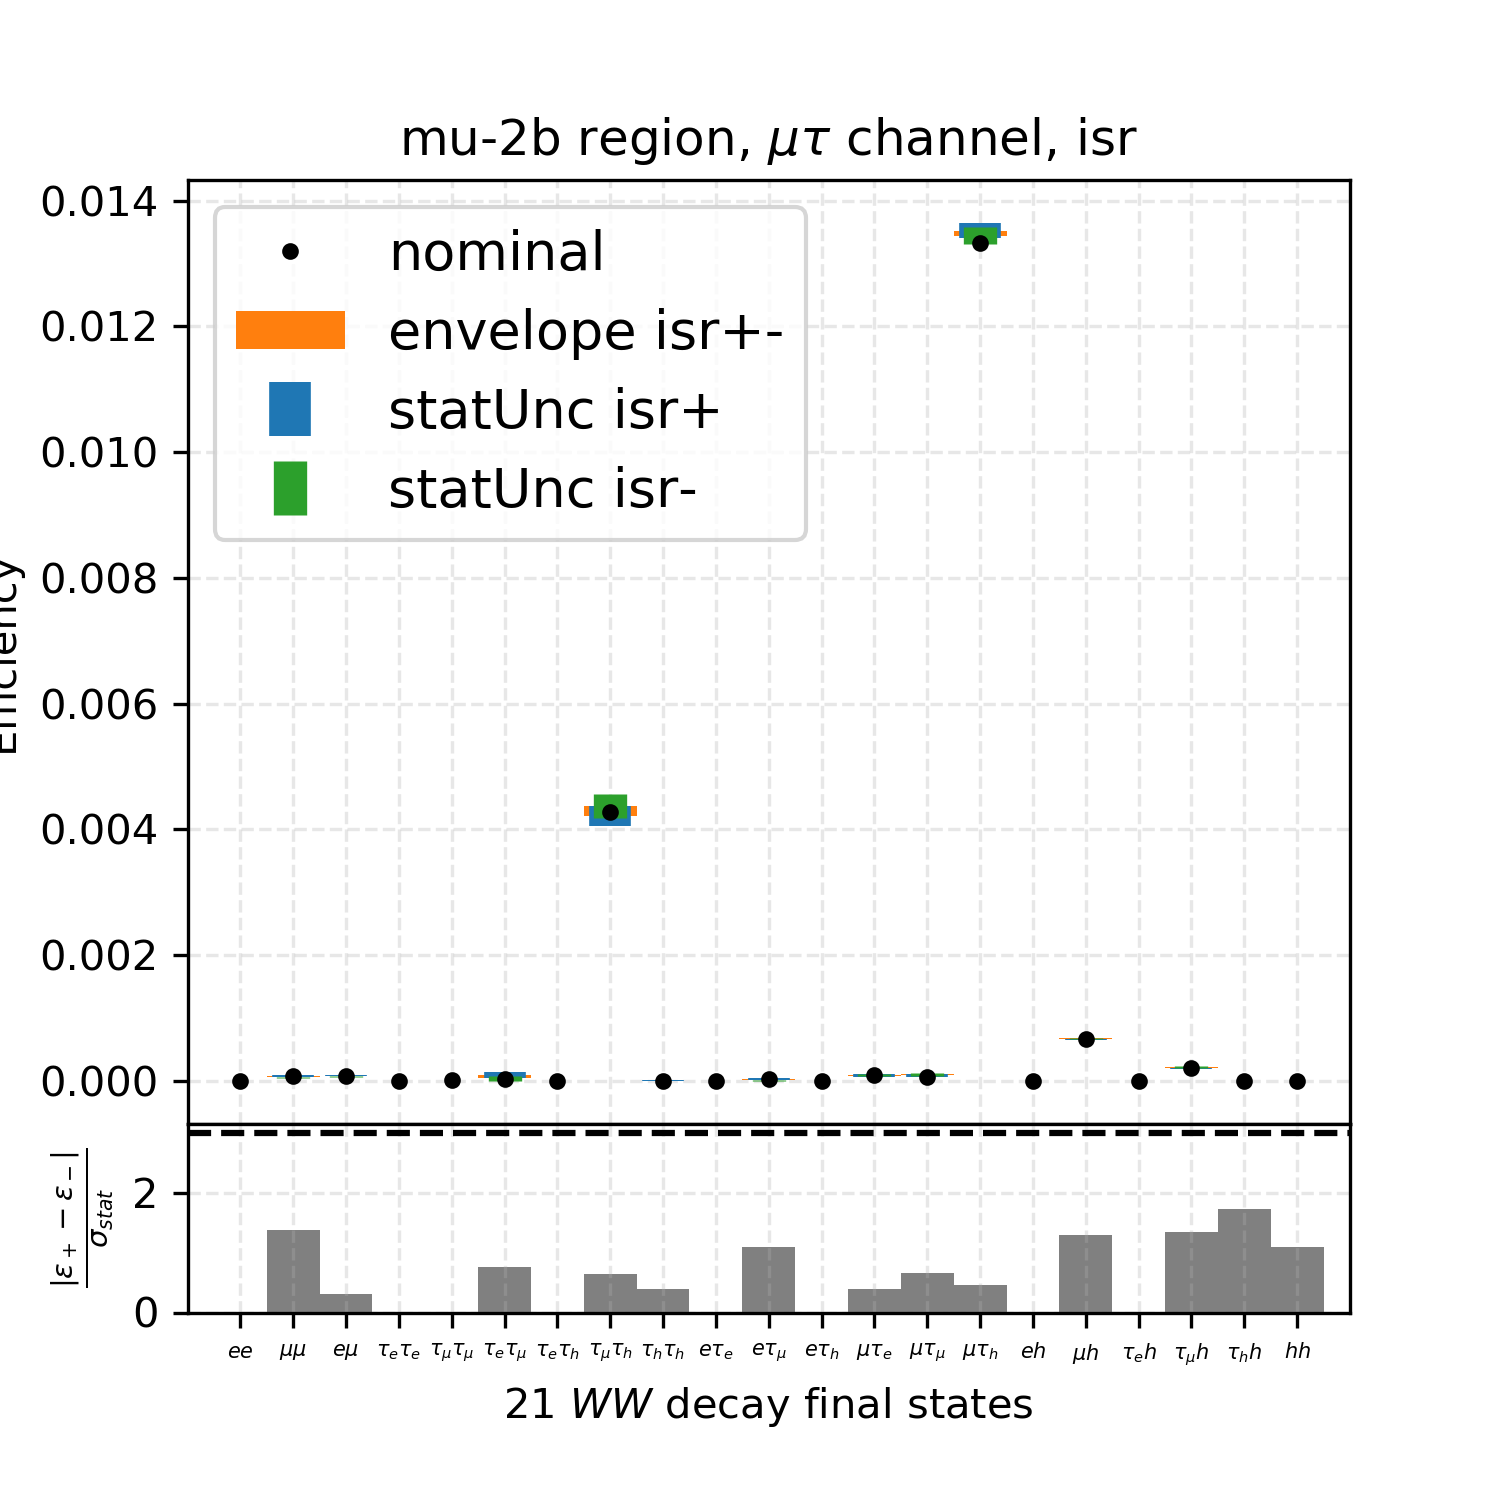
\includegraphics[width=0.24\textwidth]{chapters/Appendix/sectionTTSyst/figures/afterCorr/icata1_ch2_isr.png}
    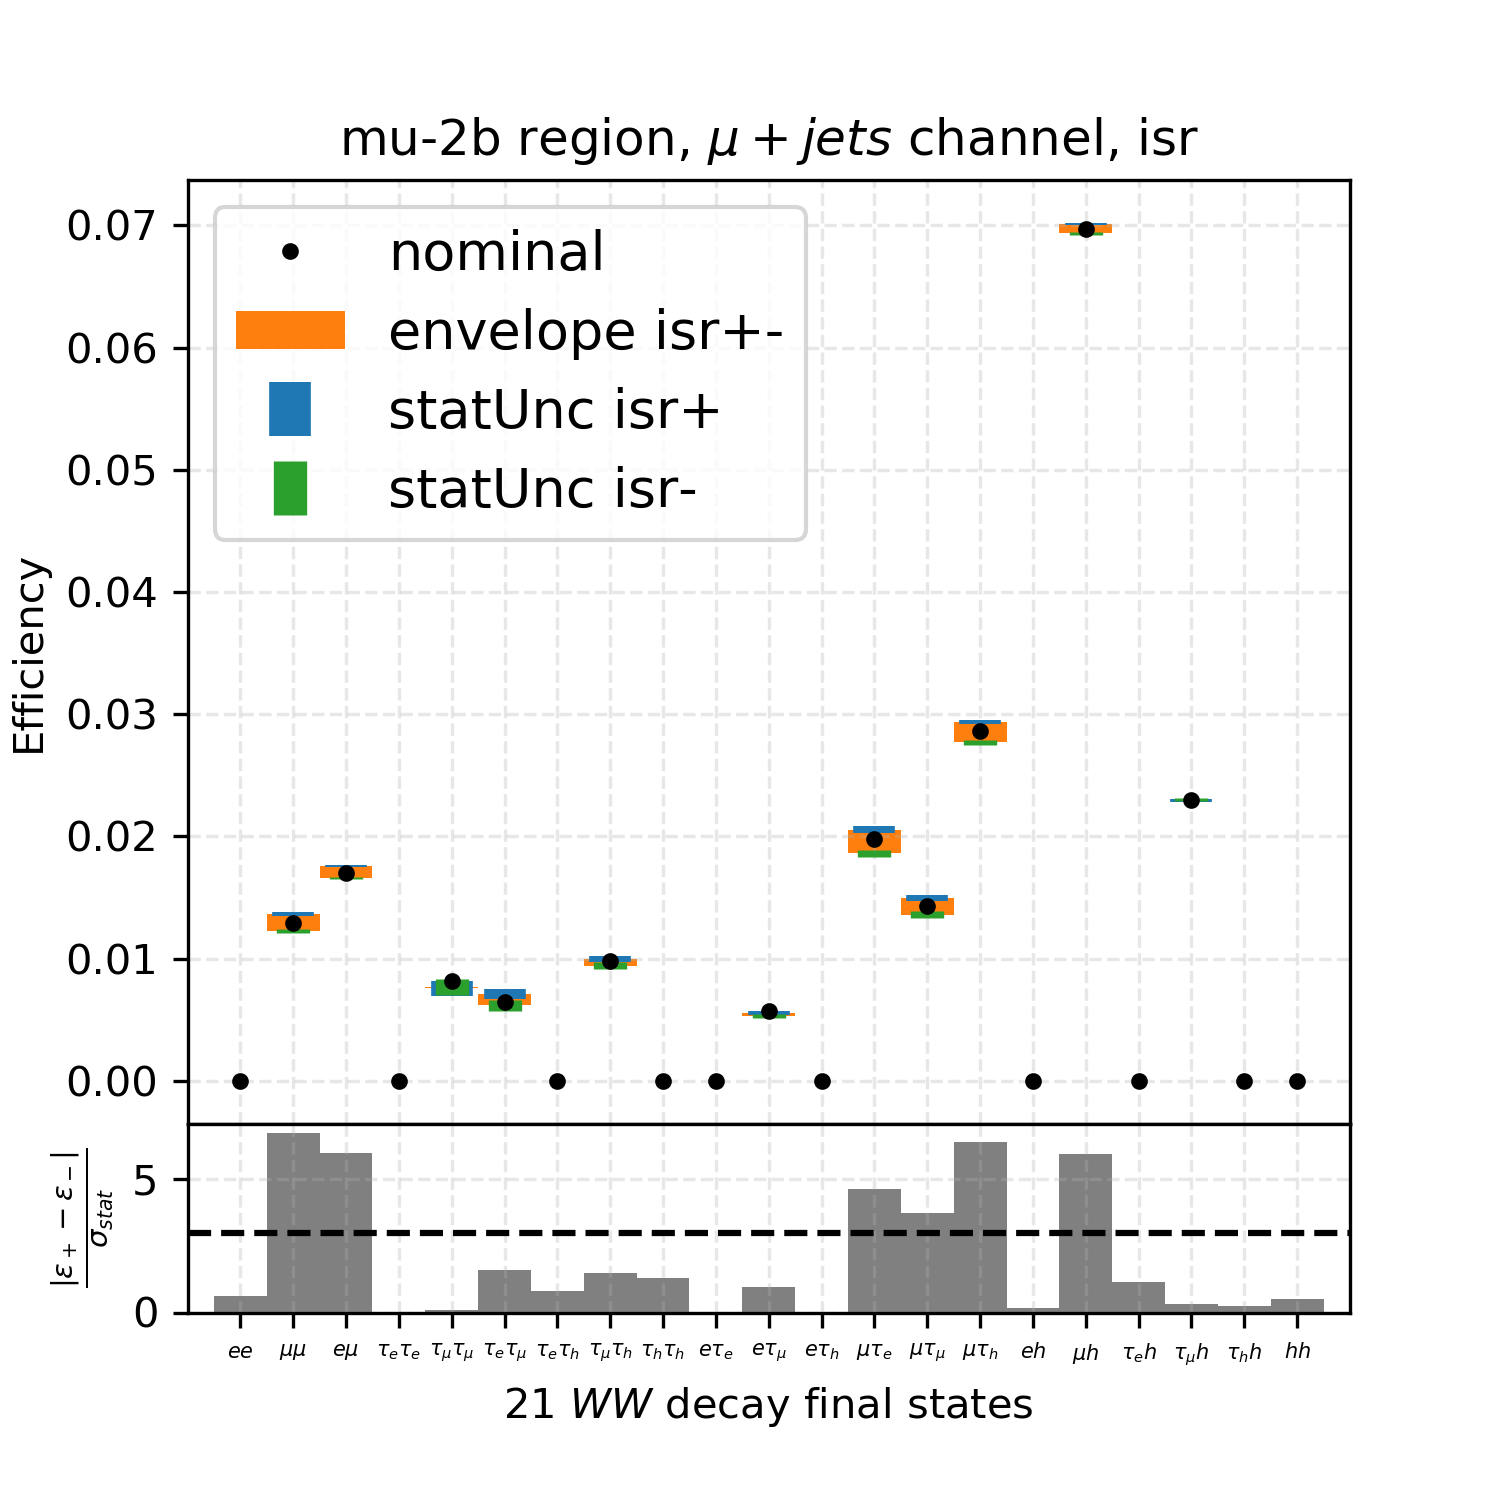
\includegraphics[width=0.24\textwidth]{chapters/Appendix/sectionTTSyst/figures/afterCorr/icata1_ch3_isr.png}
    
    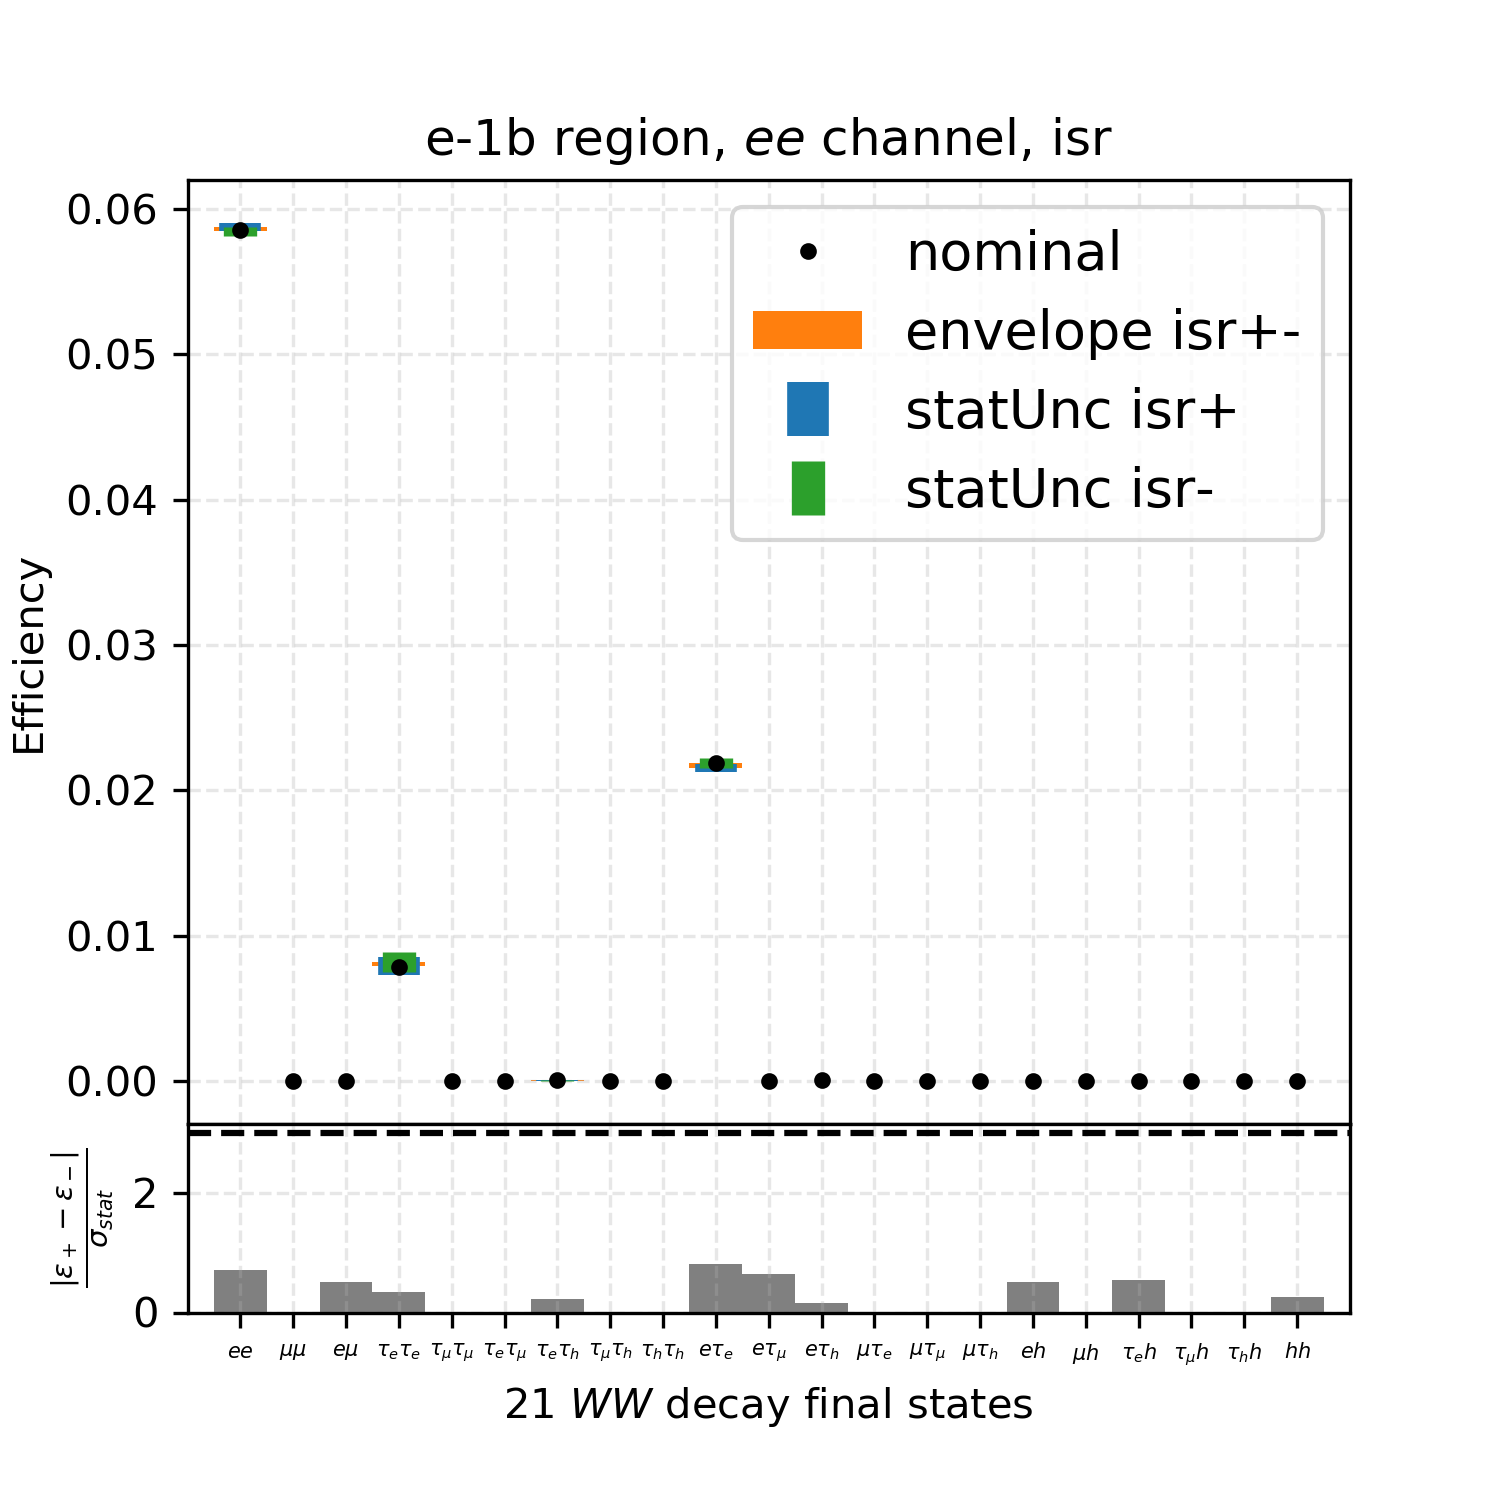
\includegraphics[width=0.24\textwidth]{chapters/Appendix/sectionTTSyst/figures/afterCorr/icata2_ch0_isr.png}
    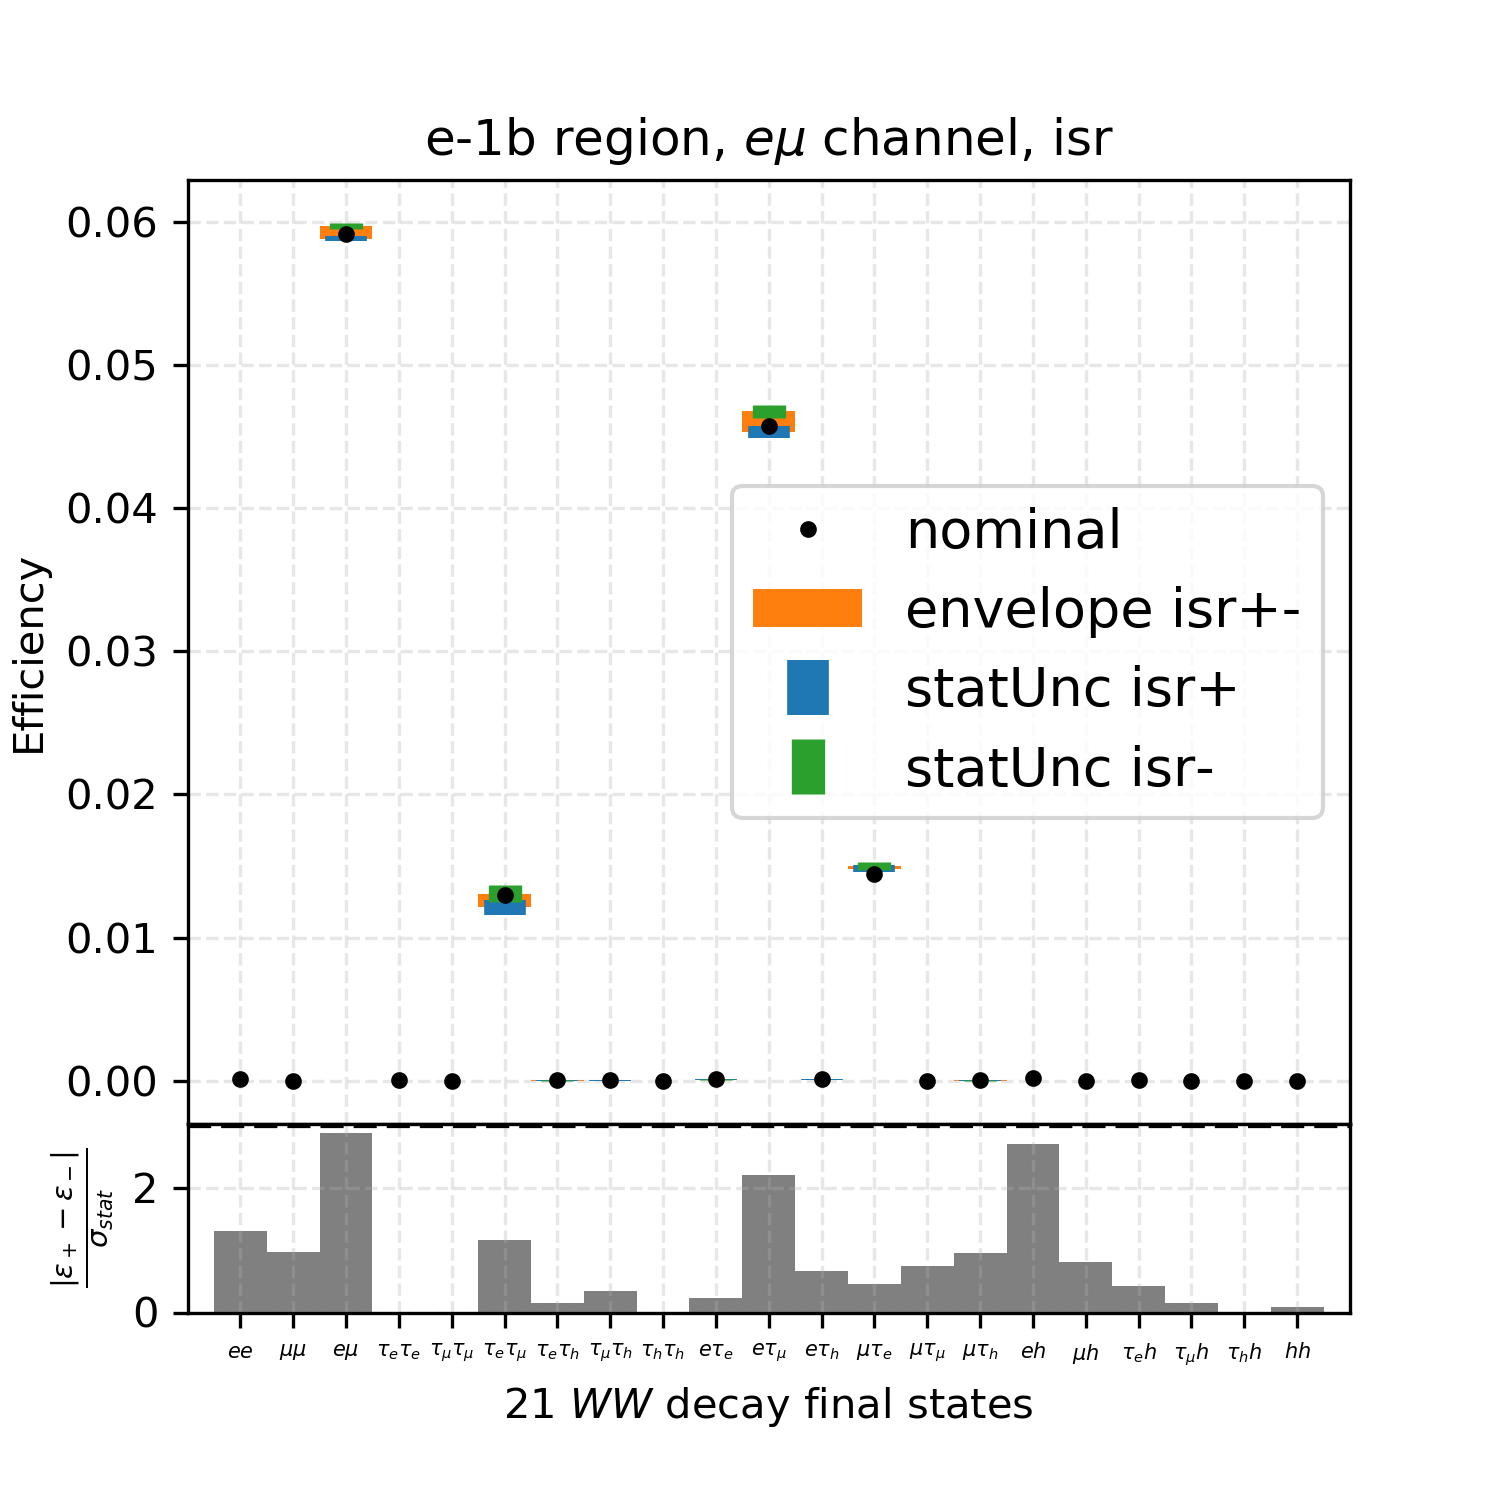
\includegraphics[width=0.24\textwidth]{chapters/Appendix/sectionTTSyst/figures/afterCorr/icata2_ch1_isr.png}
    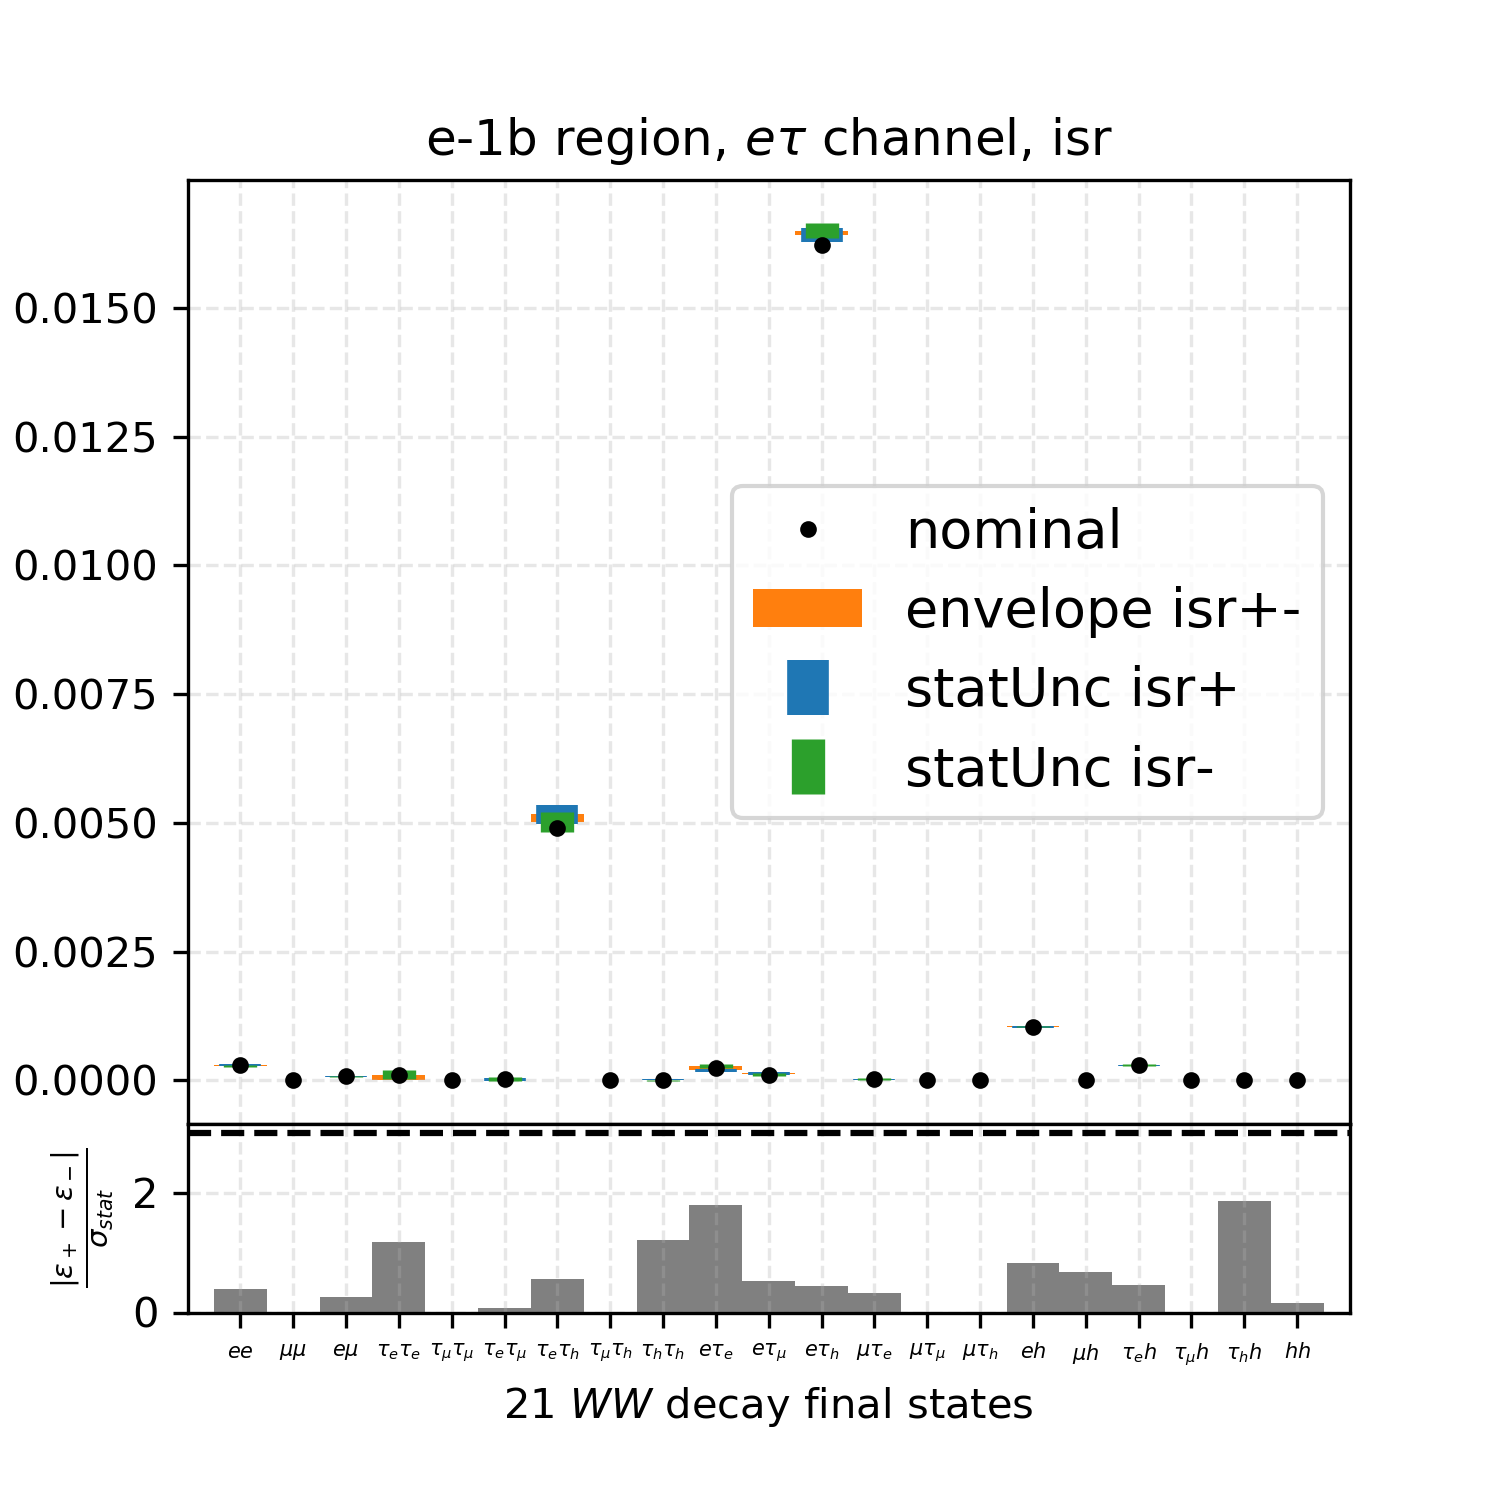
\includegraphics[width=0.24\textwidth]{chapters/Appendix/sectionTTSyst/figures/afterCorr/icata2_ch2_isr.png}
    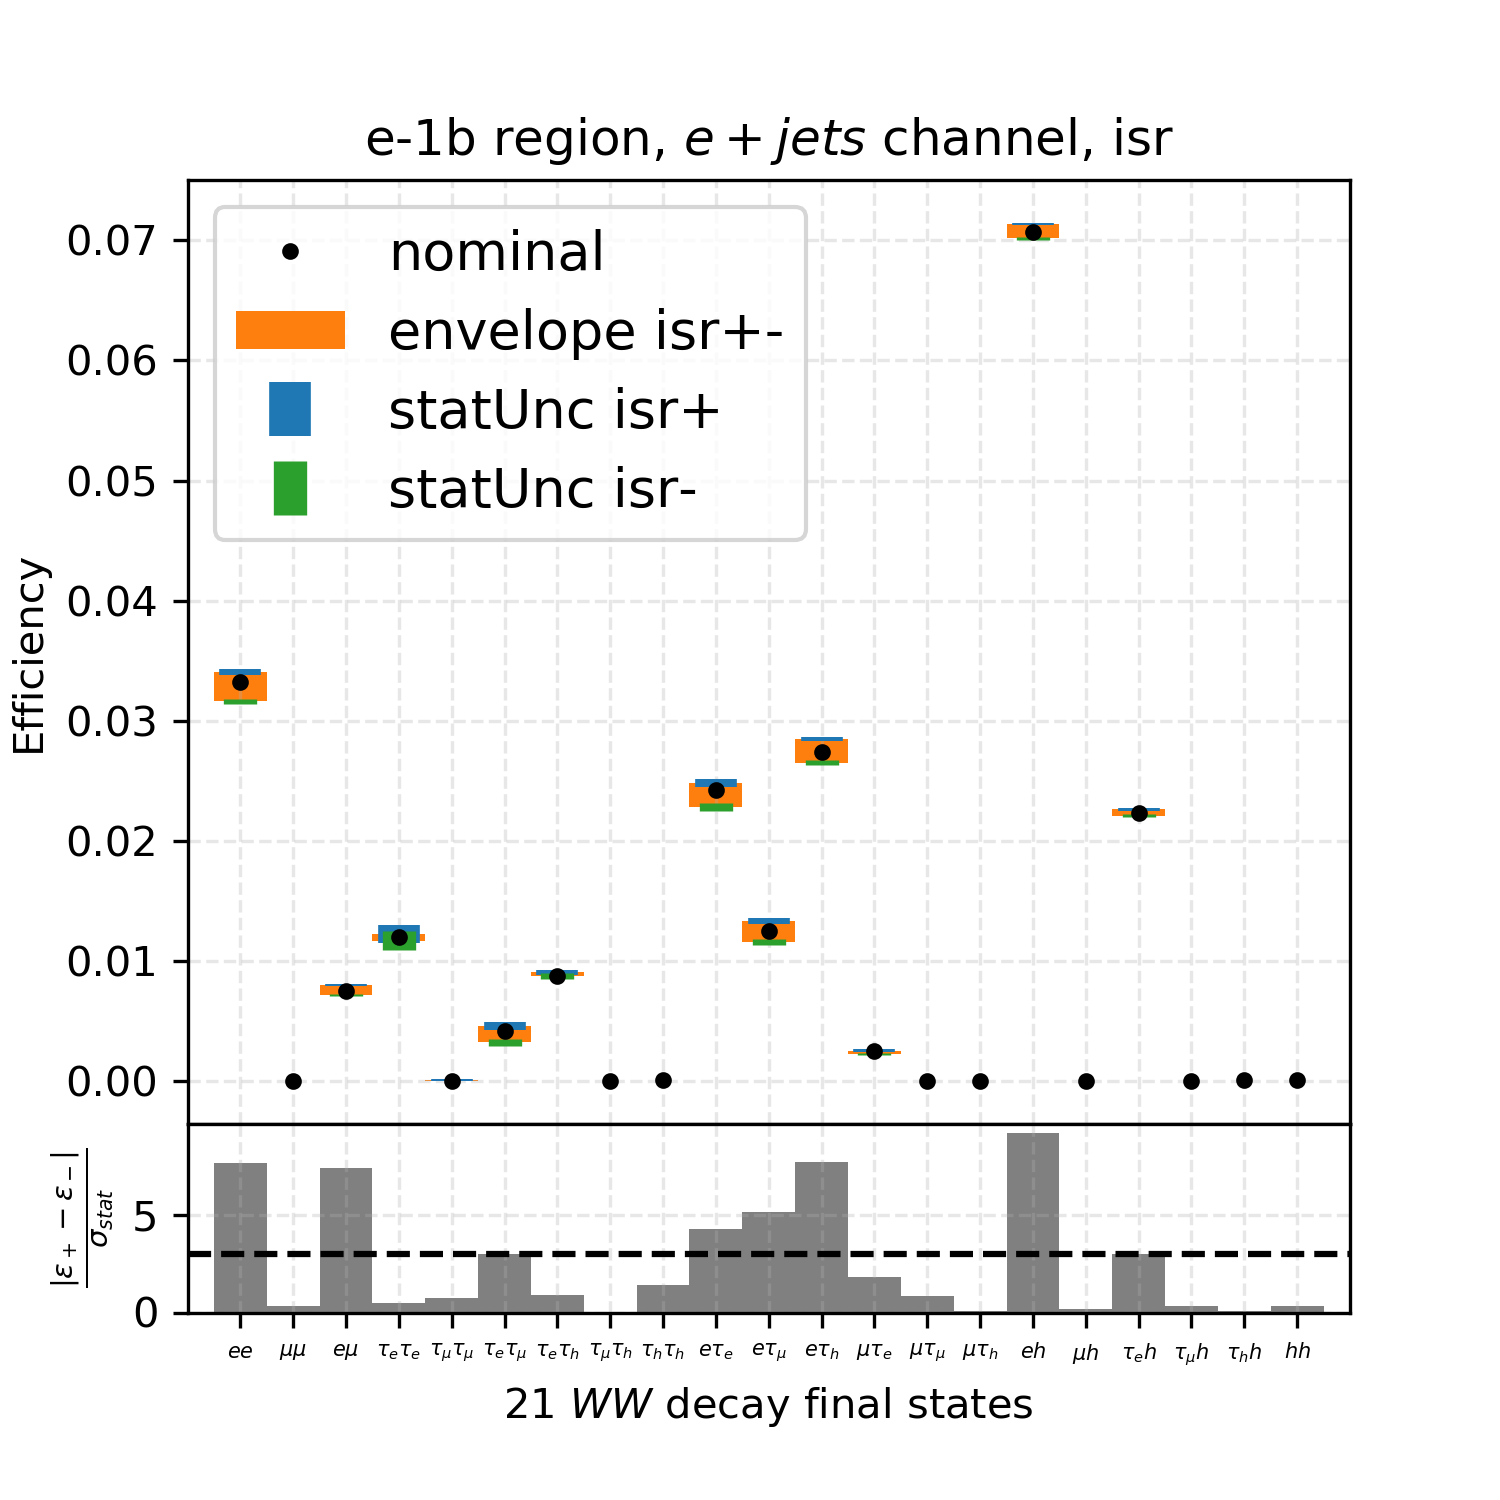
\includegraphics[width=0.24\textwidth]{chapters/Appendix/sectionTTSyst/figures/afterCorr/icata2_ch3_isr.png}

    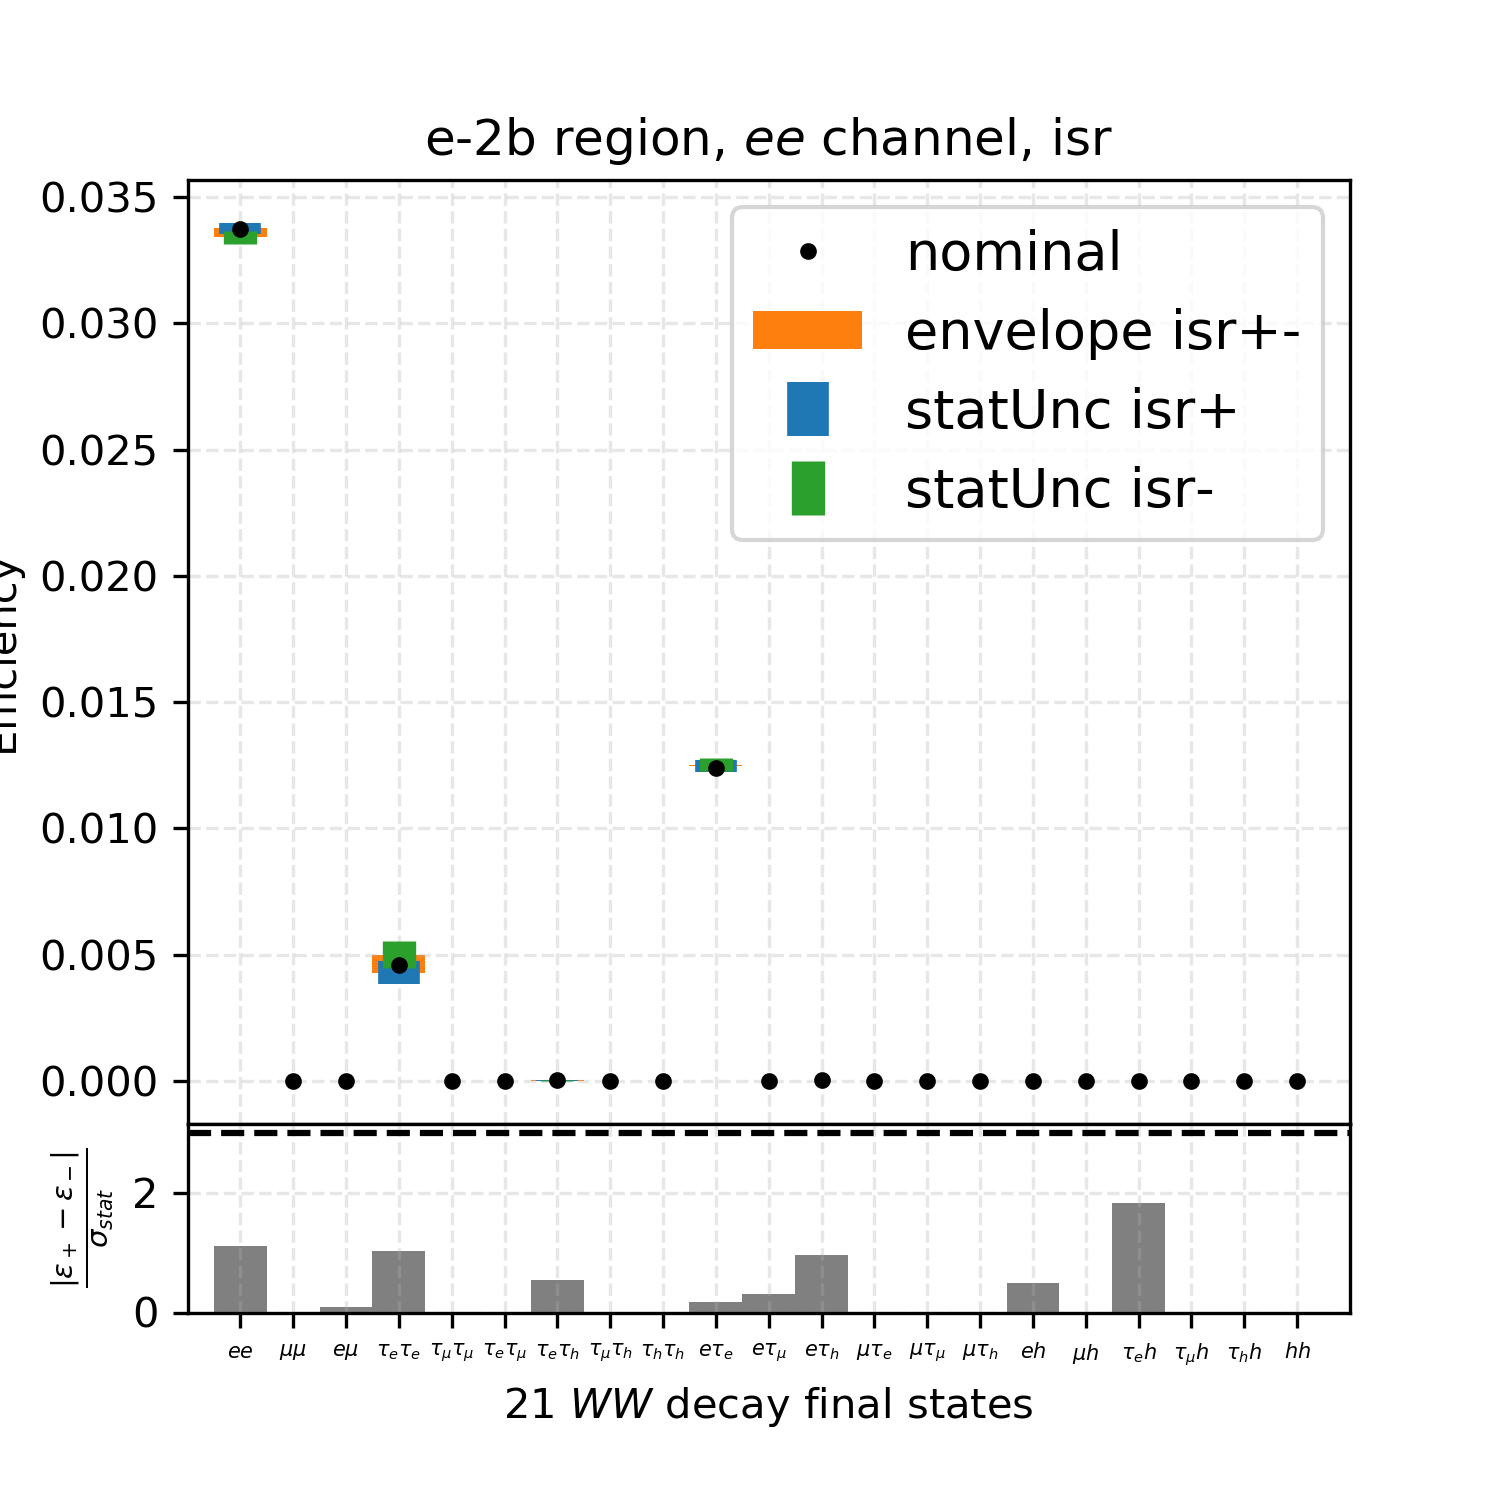
\includegraphics[width=0.24\textwidth]{chapters/Appendix/sectionTTSyst/figures/afterCorr/icata3_ch0_isr.png}
    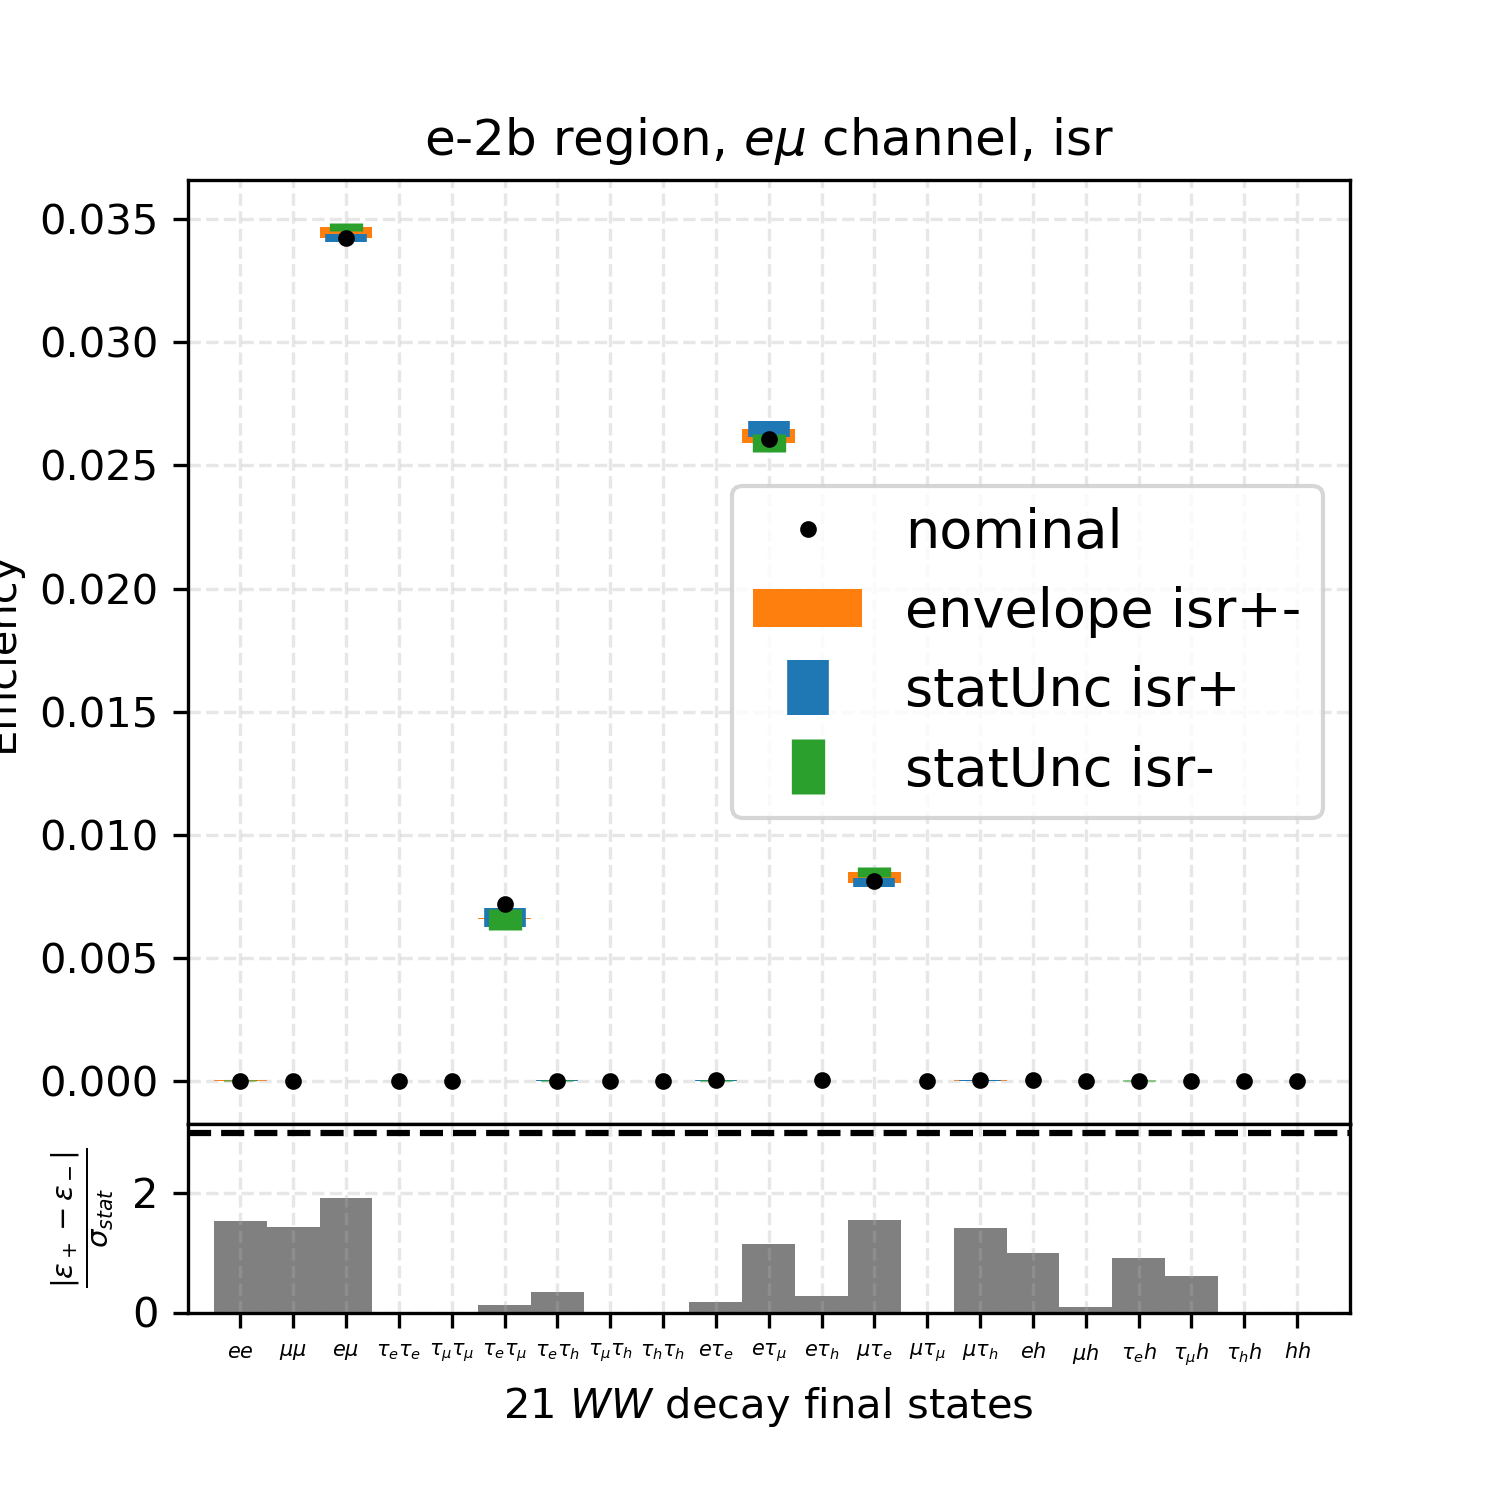
\includegraphics[width=0.24\textwidth]{chapters/Appendix/sectionTTSyst/figures/afterCorr/icata3_ch1_isr.png}
    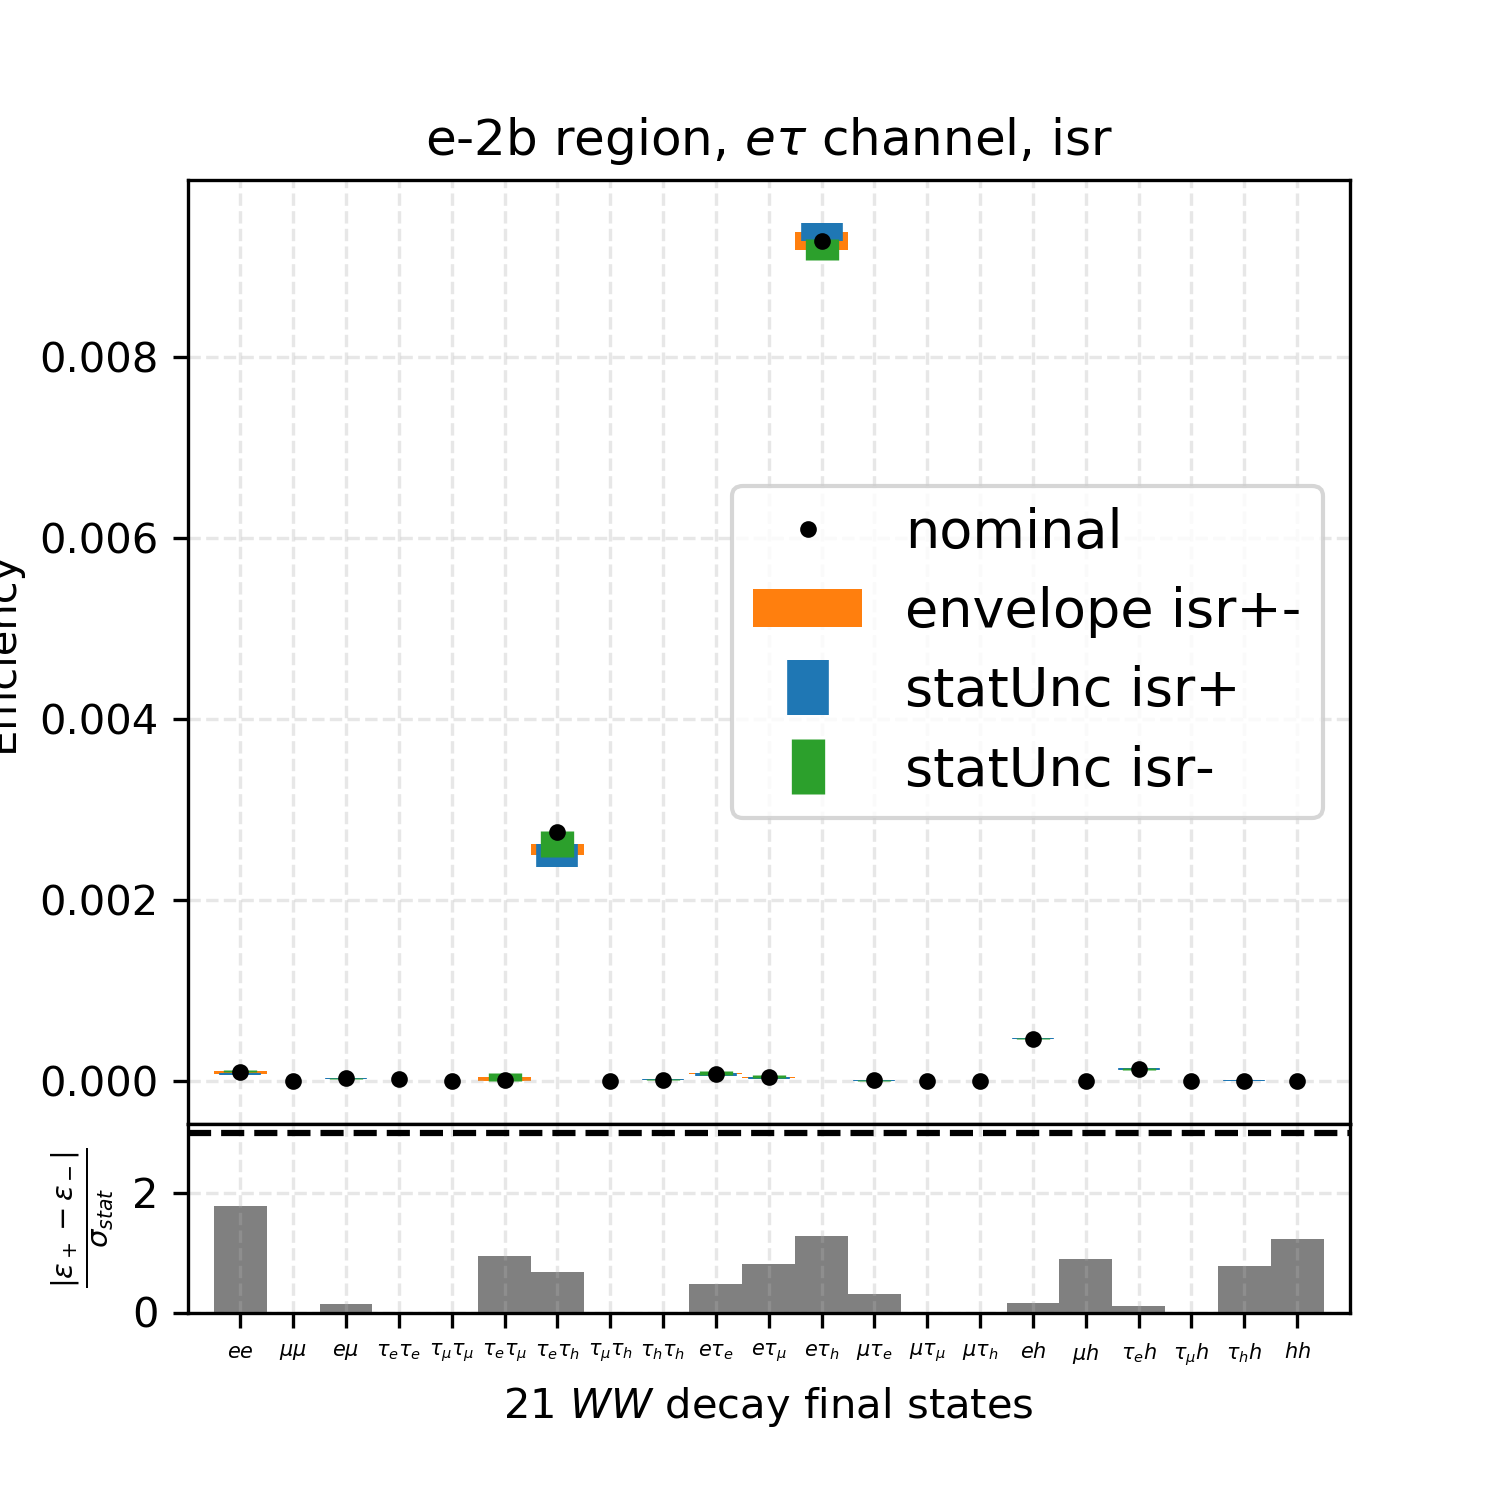
\includegraphics[width=0.24\textwidth]{chapters/Appendix/sectionTTSyst/figures/afterCorr/icata3_ch2_isr.png}
    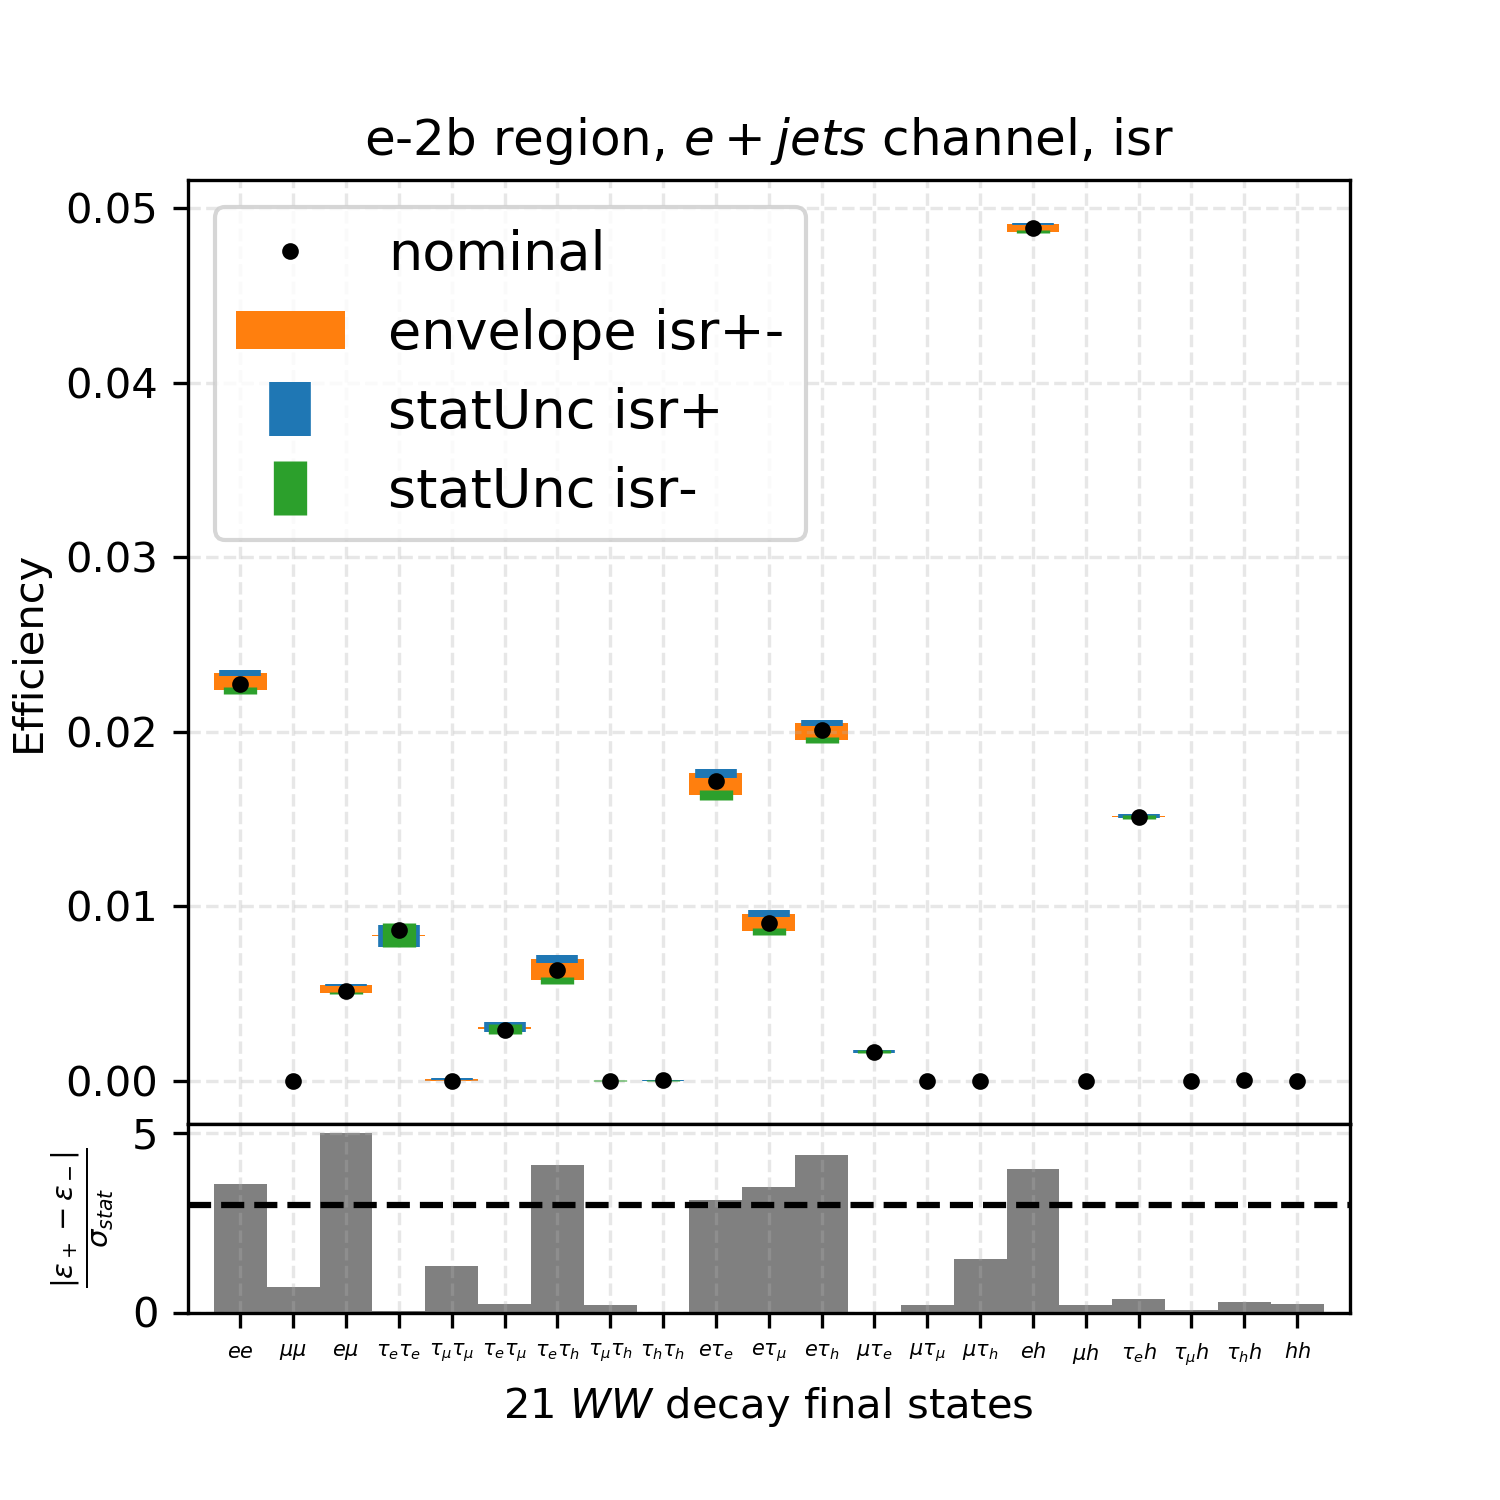
\includegraphics[width=0.24\textwidth]{chapters/Appendix/sectionTTSyst/figures/afterCorr/icata3_ch3_isr.png}
    
    \caption{Reweight $\tau_h$ and $j \to \tau_h$ efficiencies in the dedicated FSR, ISF, MEPS, UE ttbar samples}
    \label{fig:appendix:reweighttt:effAfterCorrFSR}
\end{figure}




\begin{figure}
    \centering
    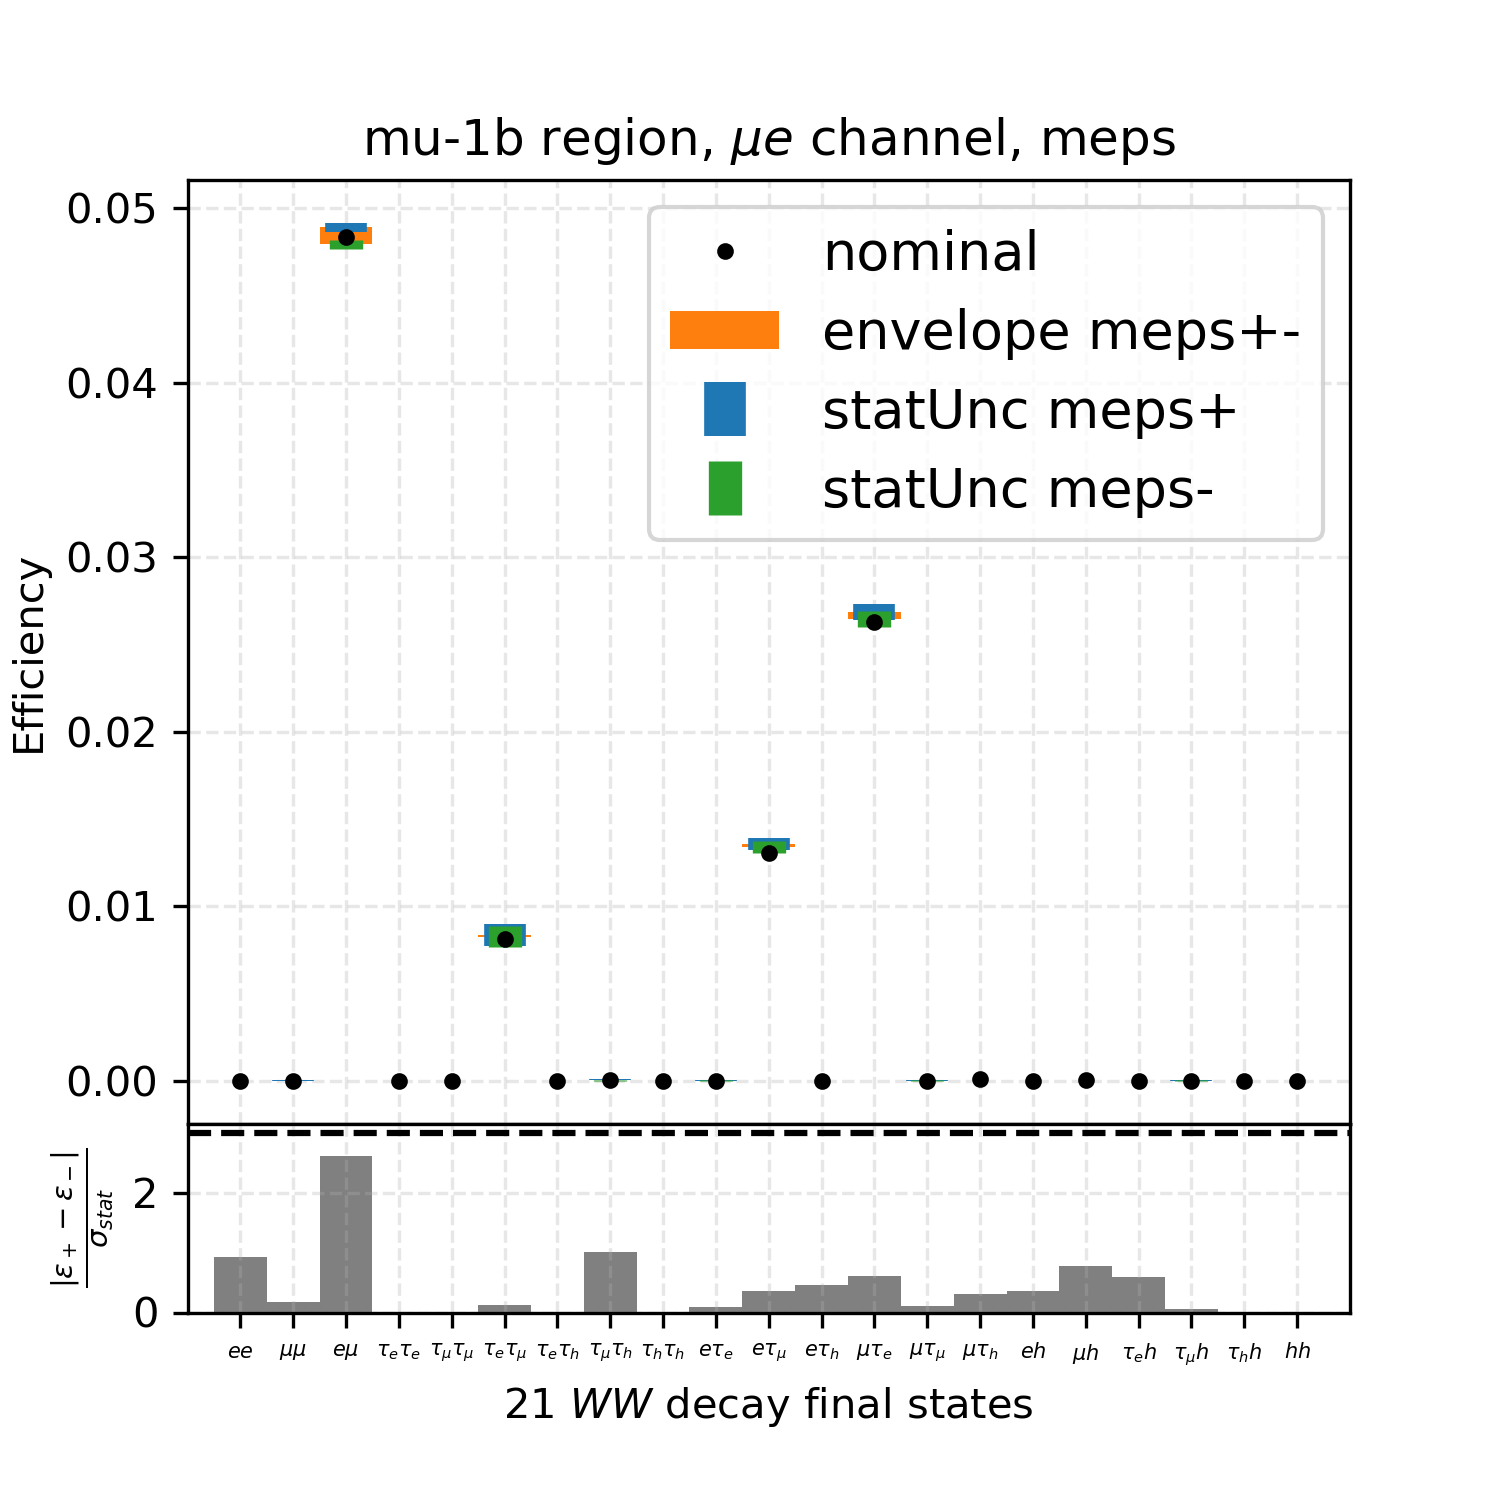
\includegraphics[width=0.24\textwidth]{chapters/Appendix/sectionTTSyst/figures/afterCorr/icata0_ch0_meps.png}
    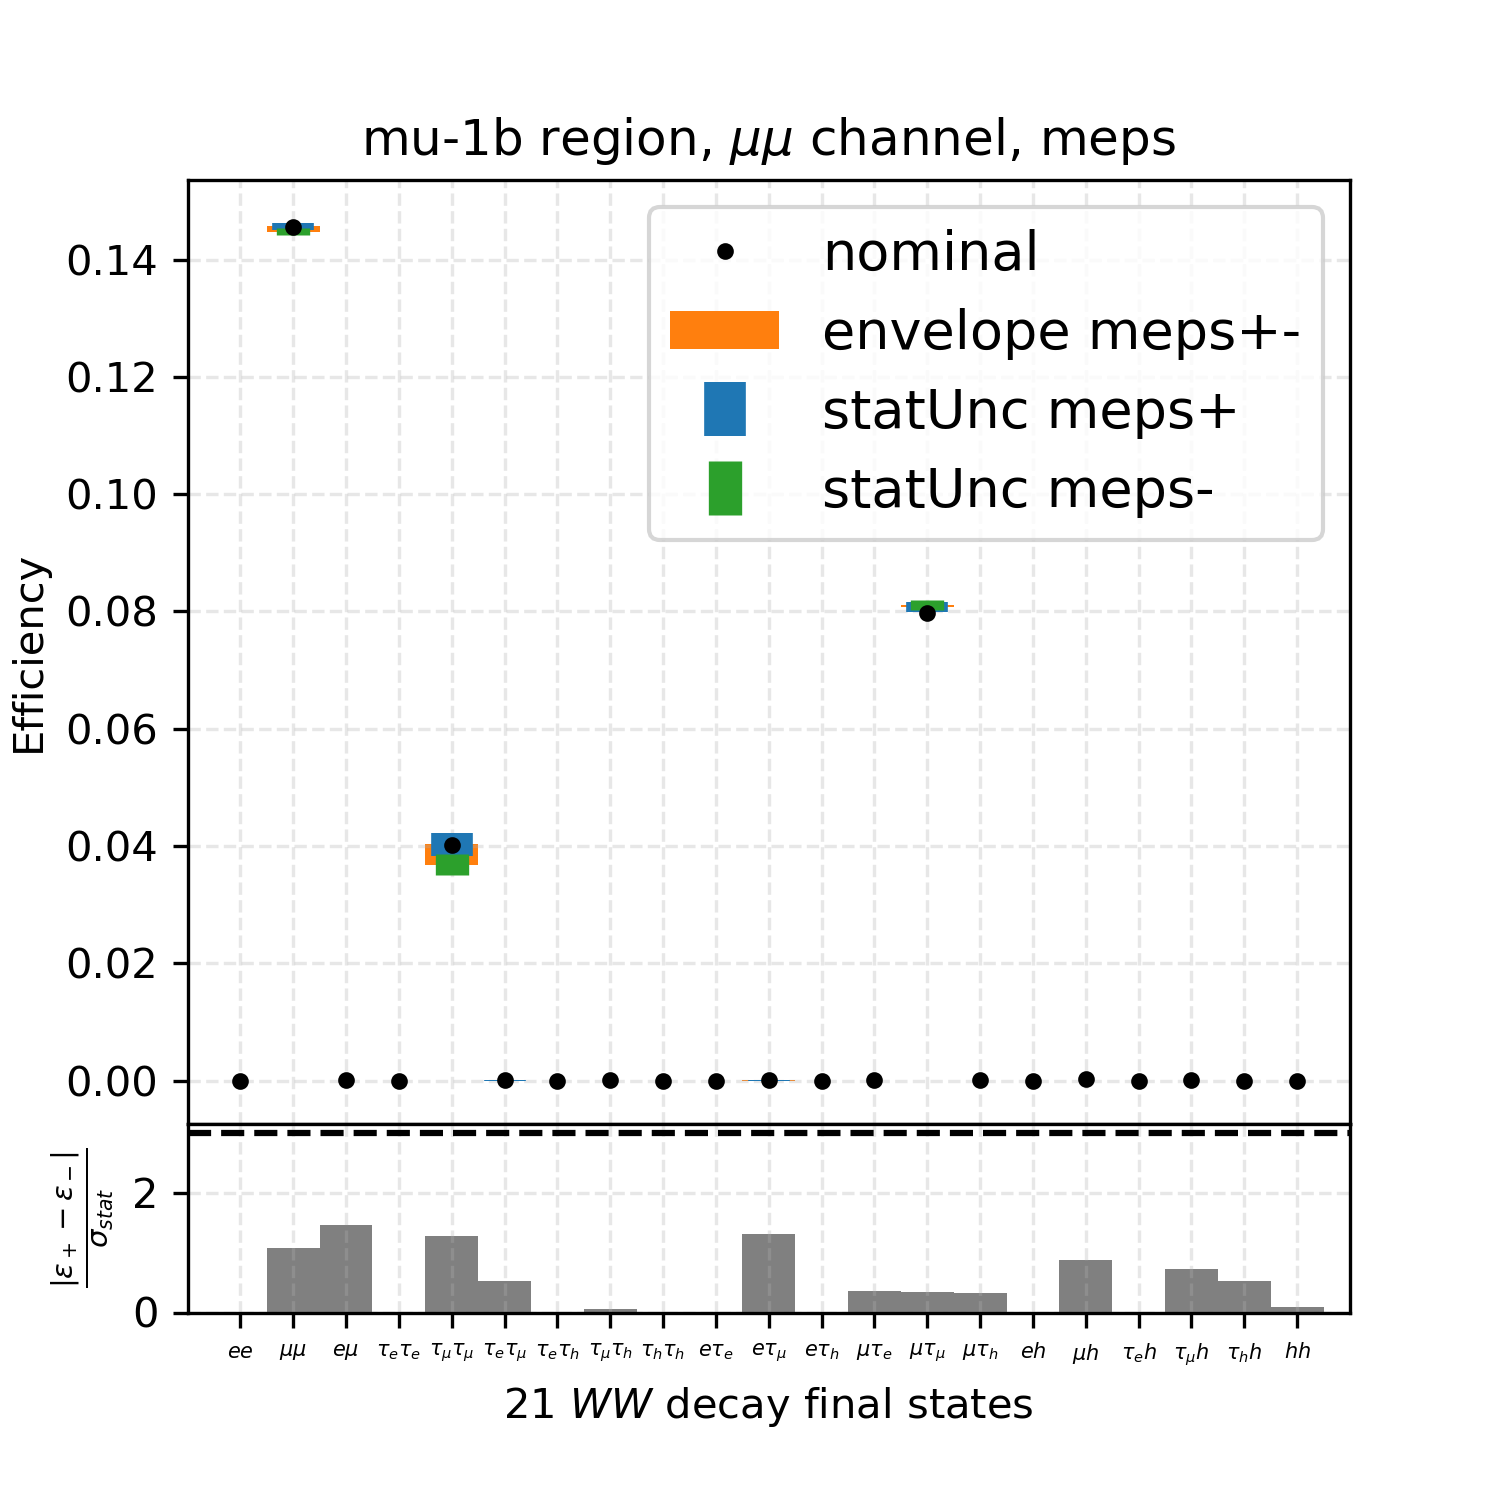
\includegraphics[width=0.24\textwidth]{chapters/Appendix/sectionTTSyst/figures/afterCorr/icata0_ch1_meps.png}
    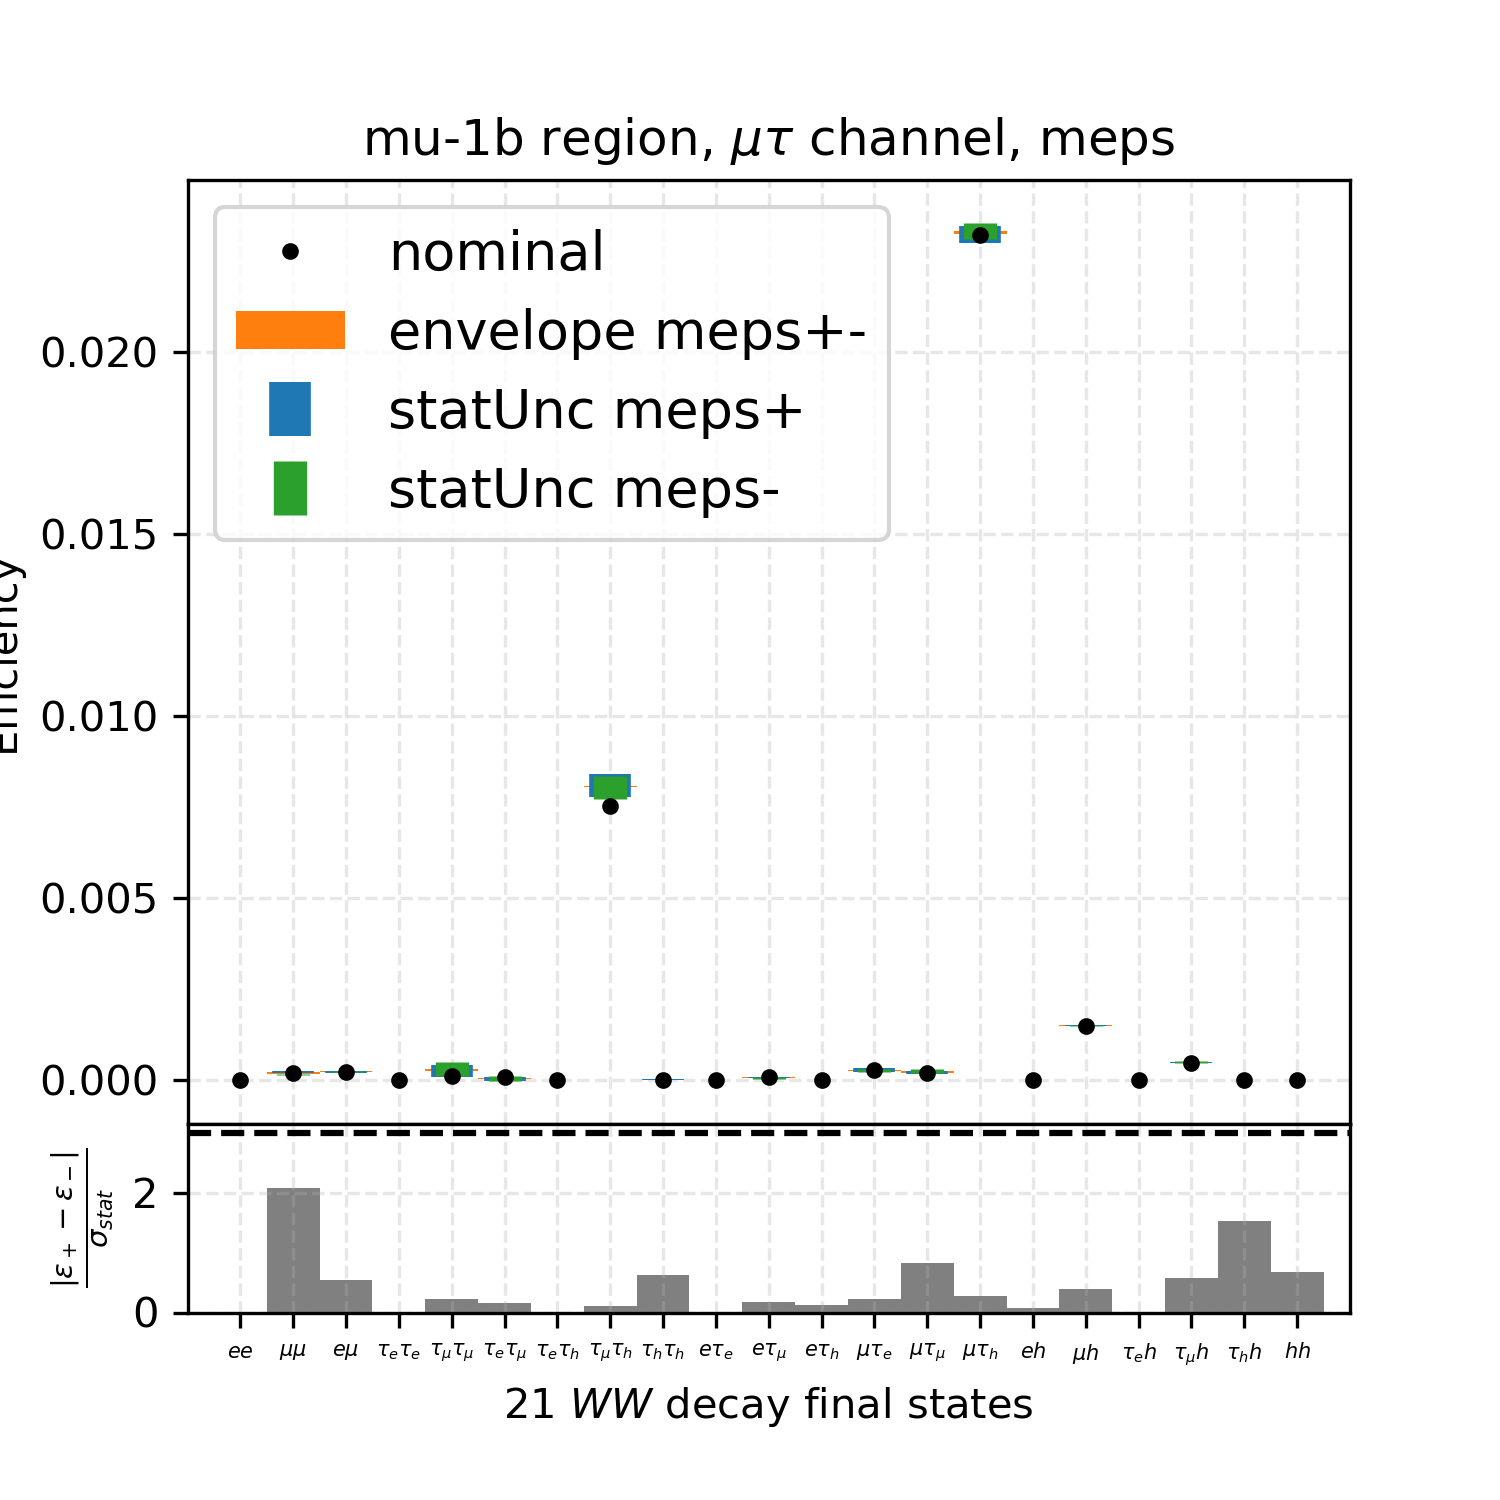
\includegraphics[width=0.24\textwidth]{chapters/Appendix/sectionTTSyst/figures/afterCorr/icata0_ch2_meps.png}
    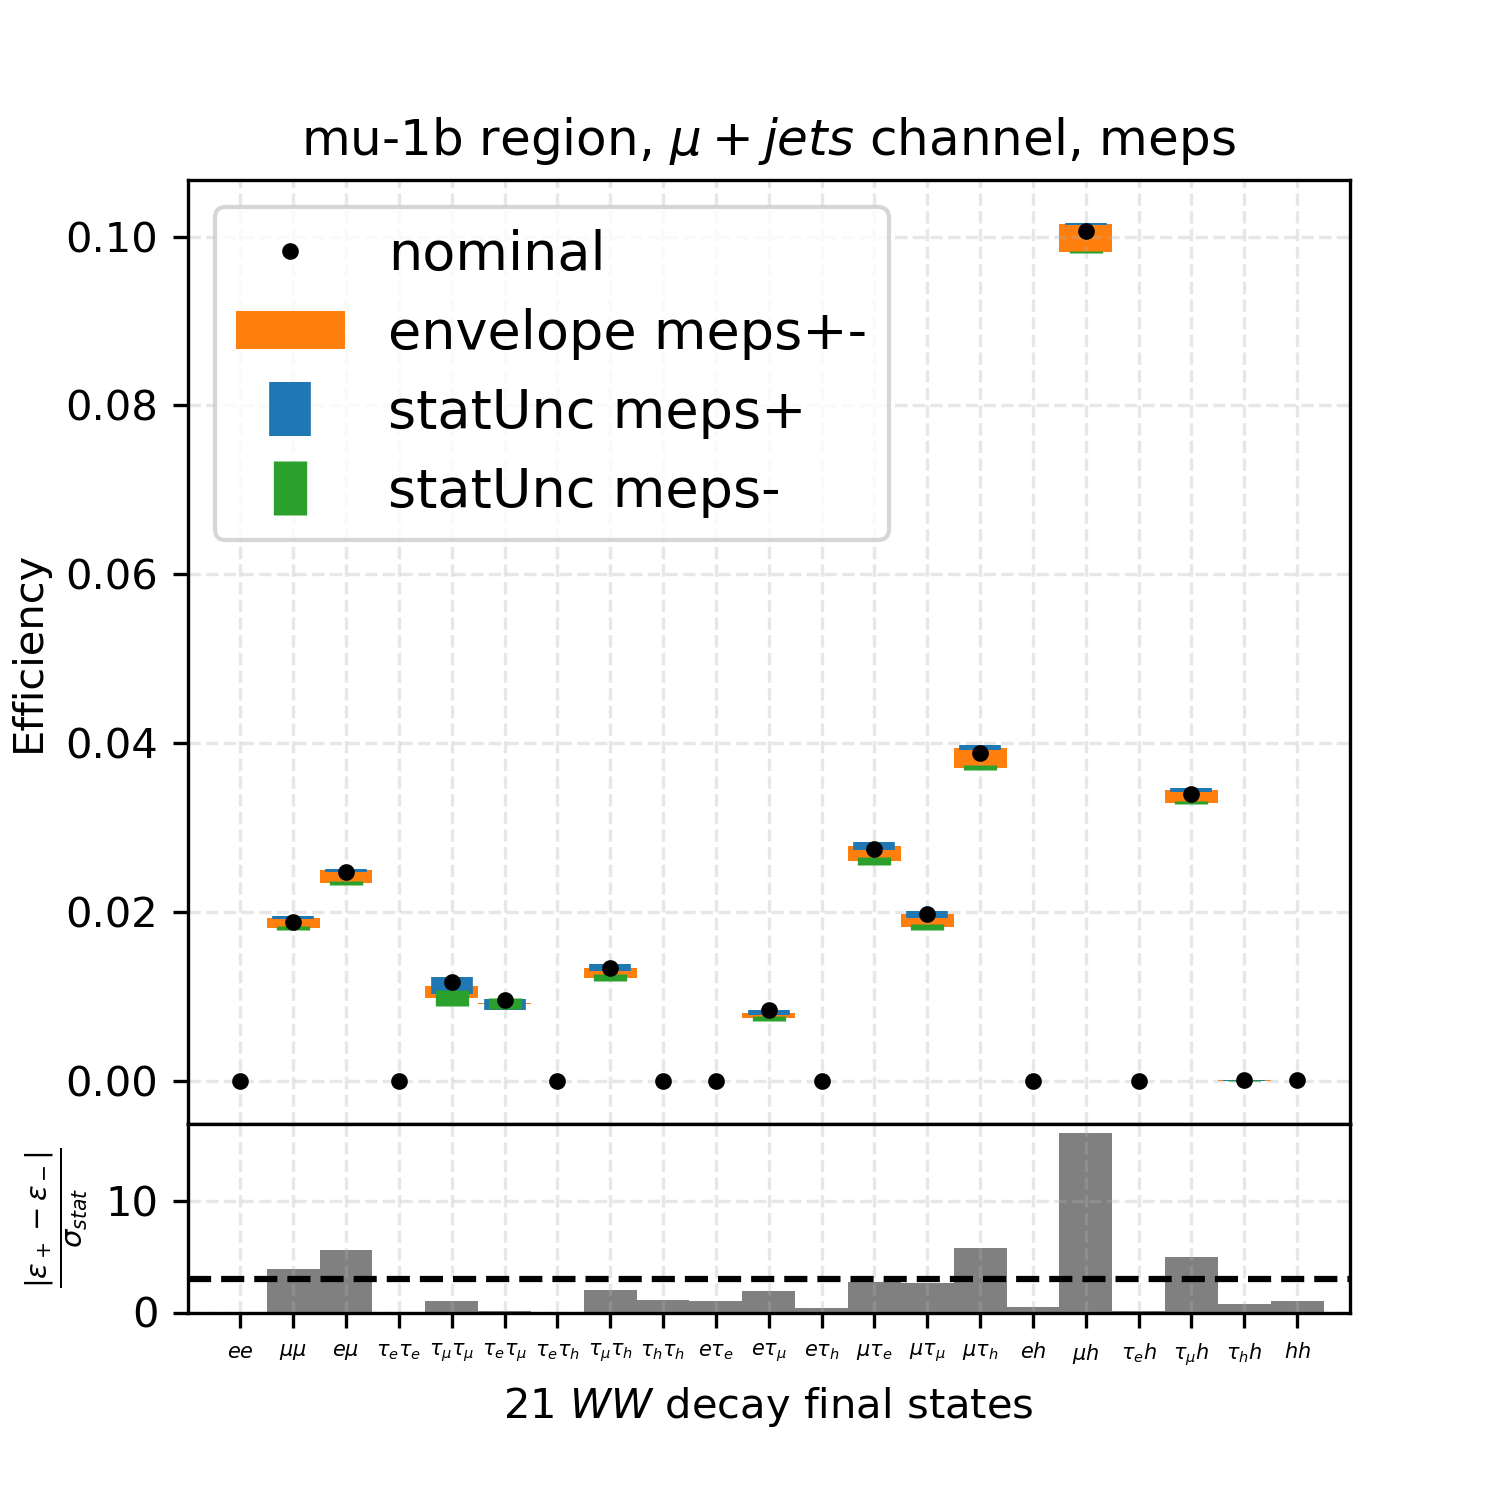
\includegraphics[width=0.24\textwidth]{chapters/Appendix/sectionTTSyst/figures/afterCorr/icata0_ch3_meps.png}

    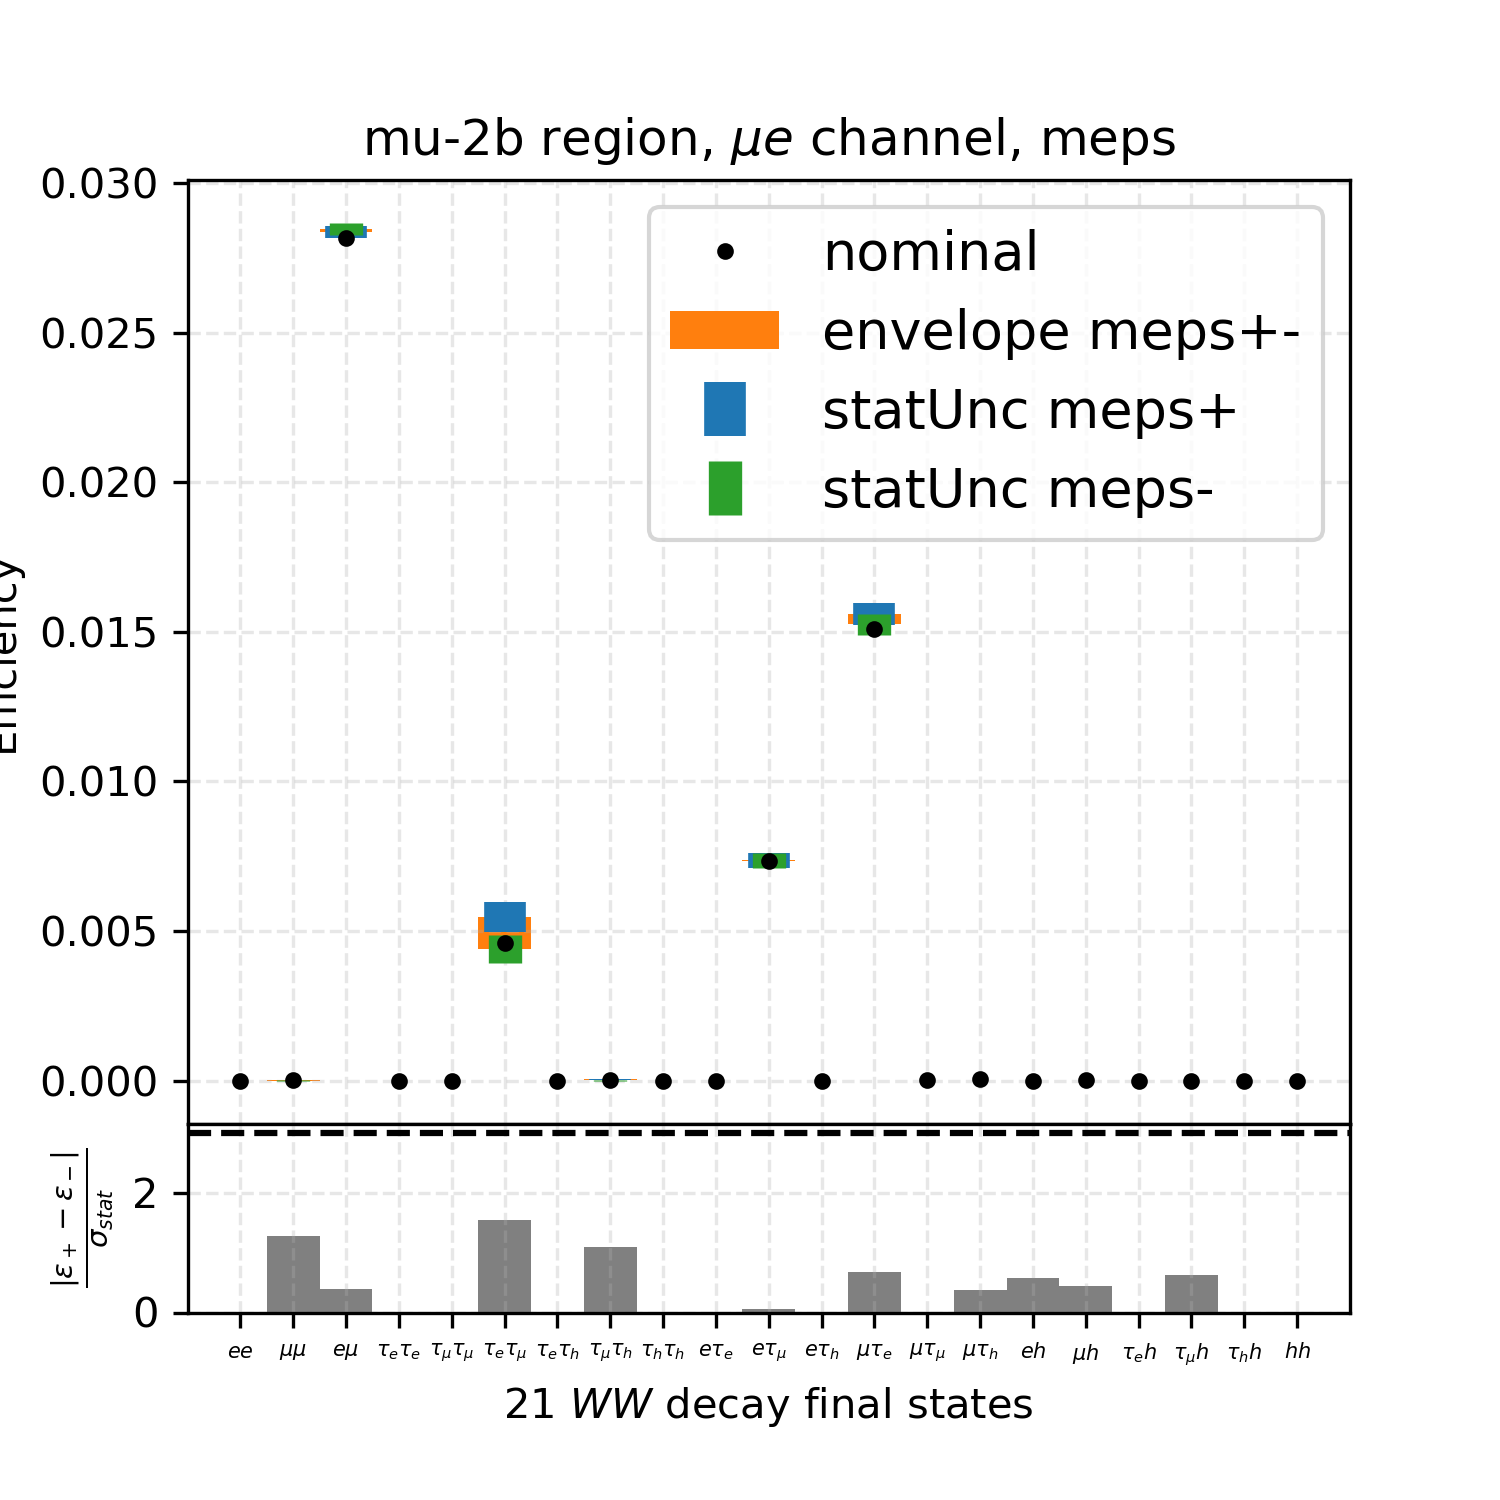
\includegraphics[width=0.24\textwidth]{chapters/Appendix/sectionTTSyst/figures/afterCorr/icata1_ch0_meps.png}
    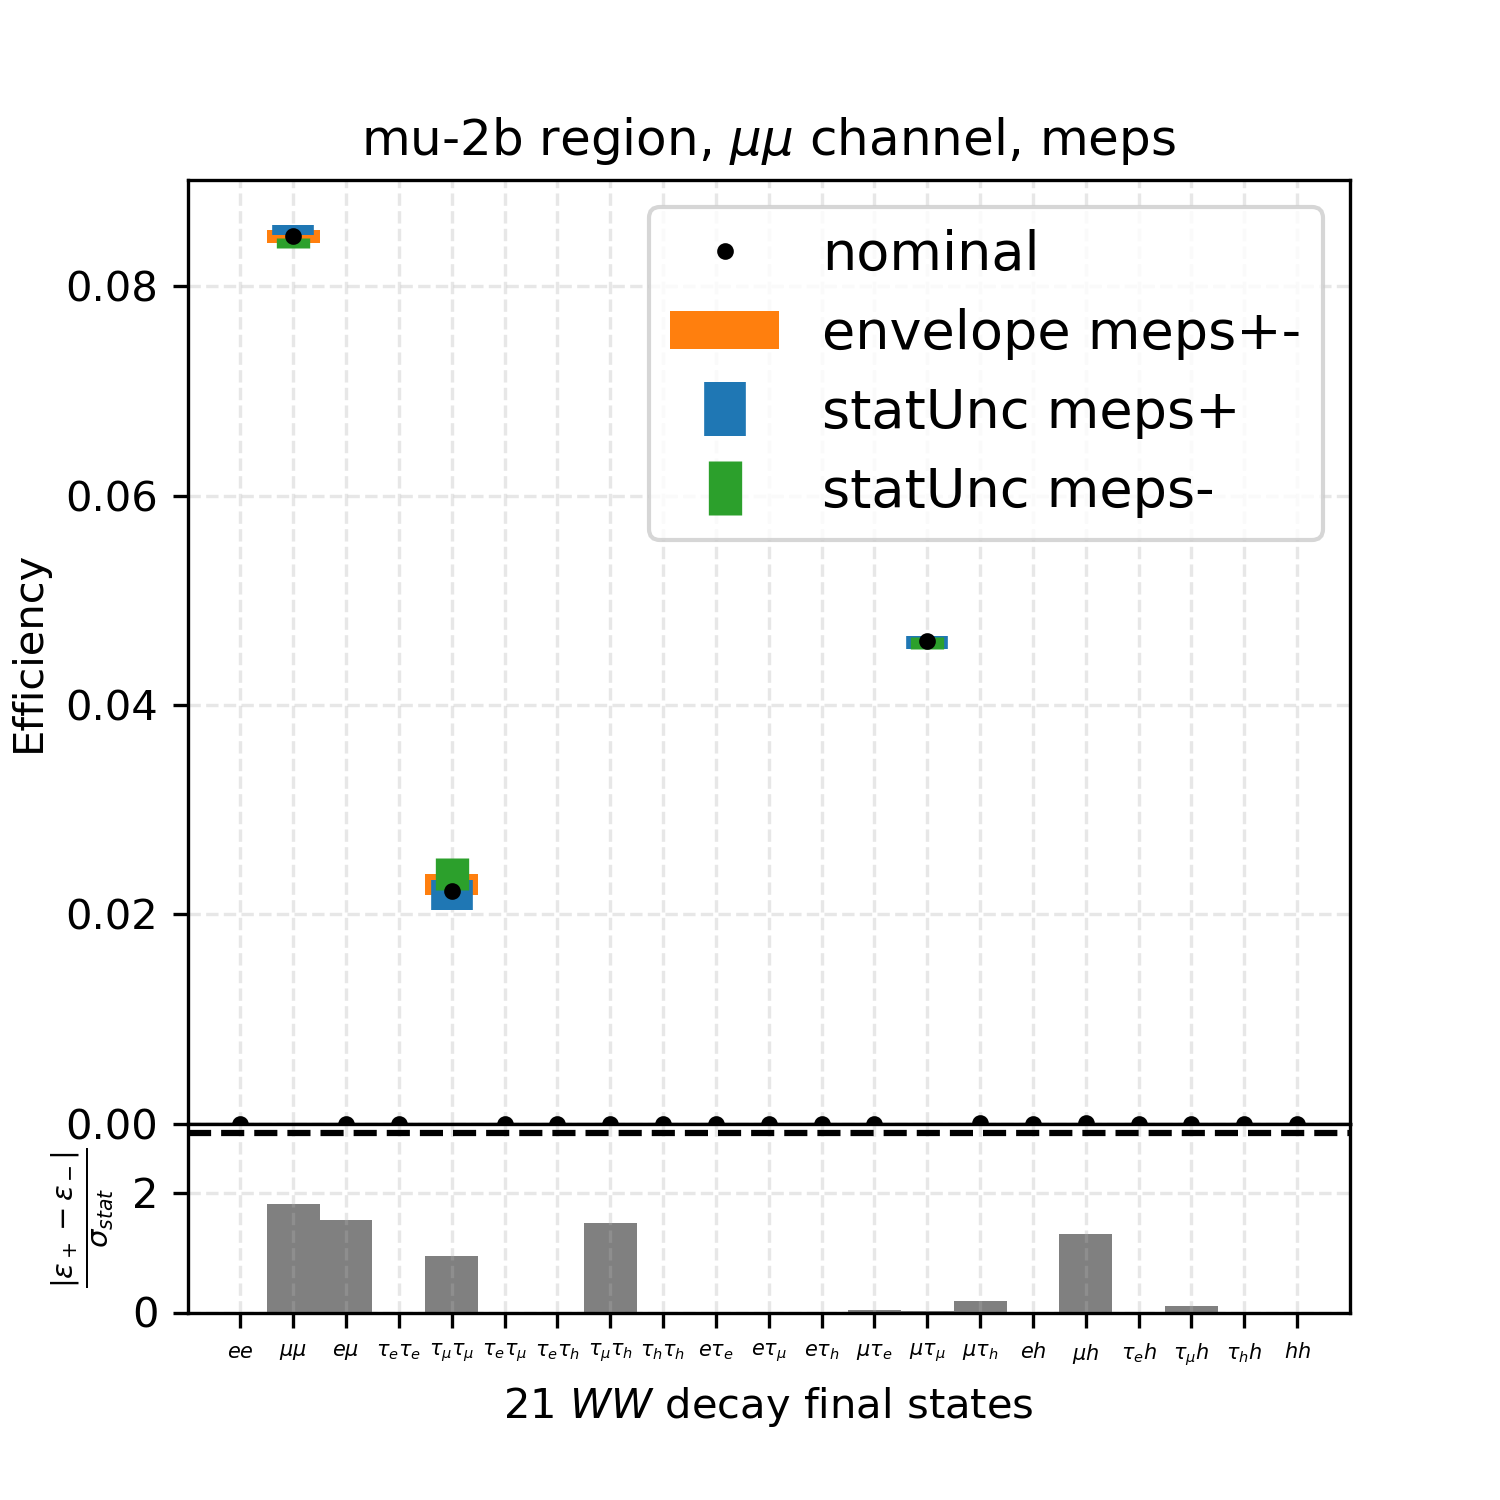
\includegraphics[width=0.24\textwidth]{chapters/Appendix/sectionTTSyst/figures/afterCorr/icata1_ch1_meps.png}
    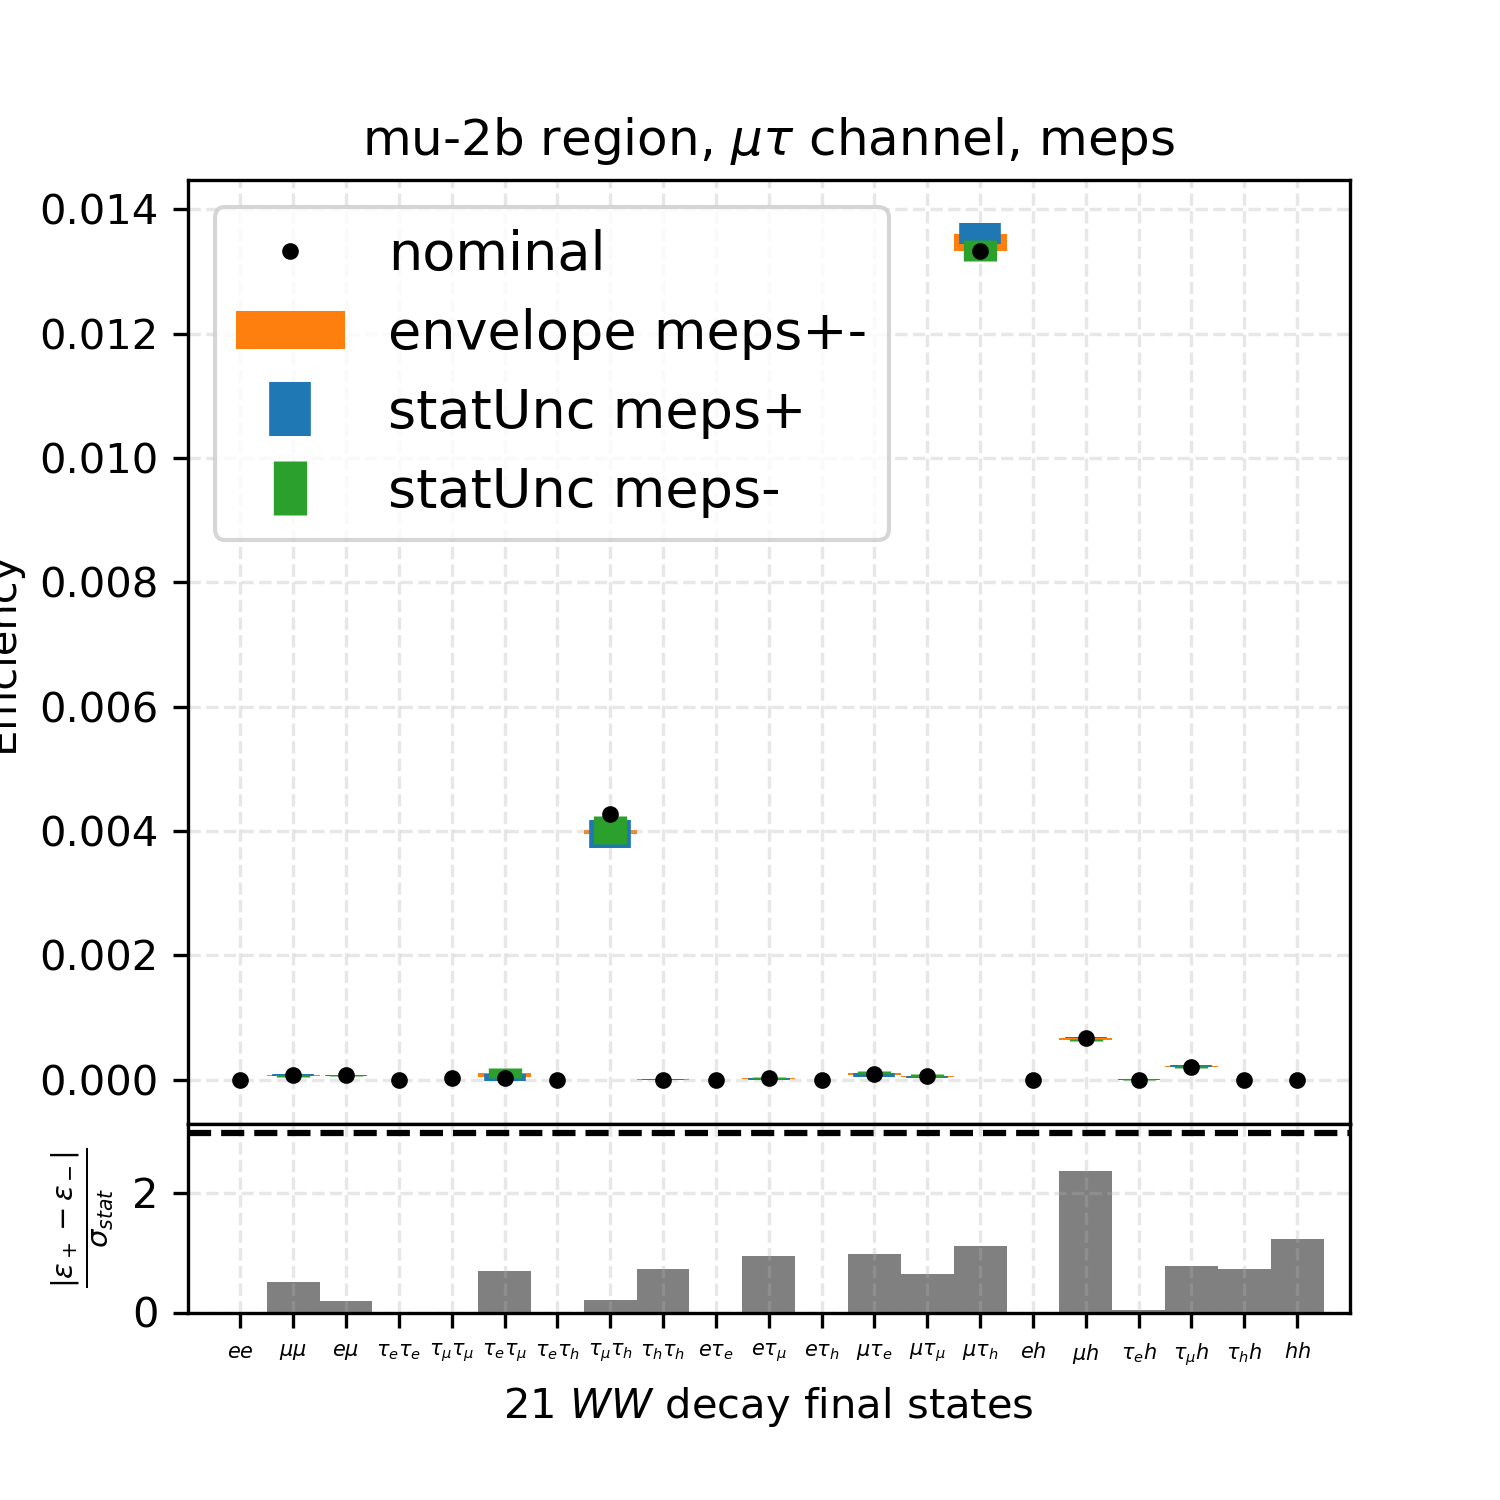
\includegraphics[width=0.24\textwidth]{chapters/Appendix/sectionTTSyst/figures/afterCorr/icata1_ch2_meps.png}
    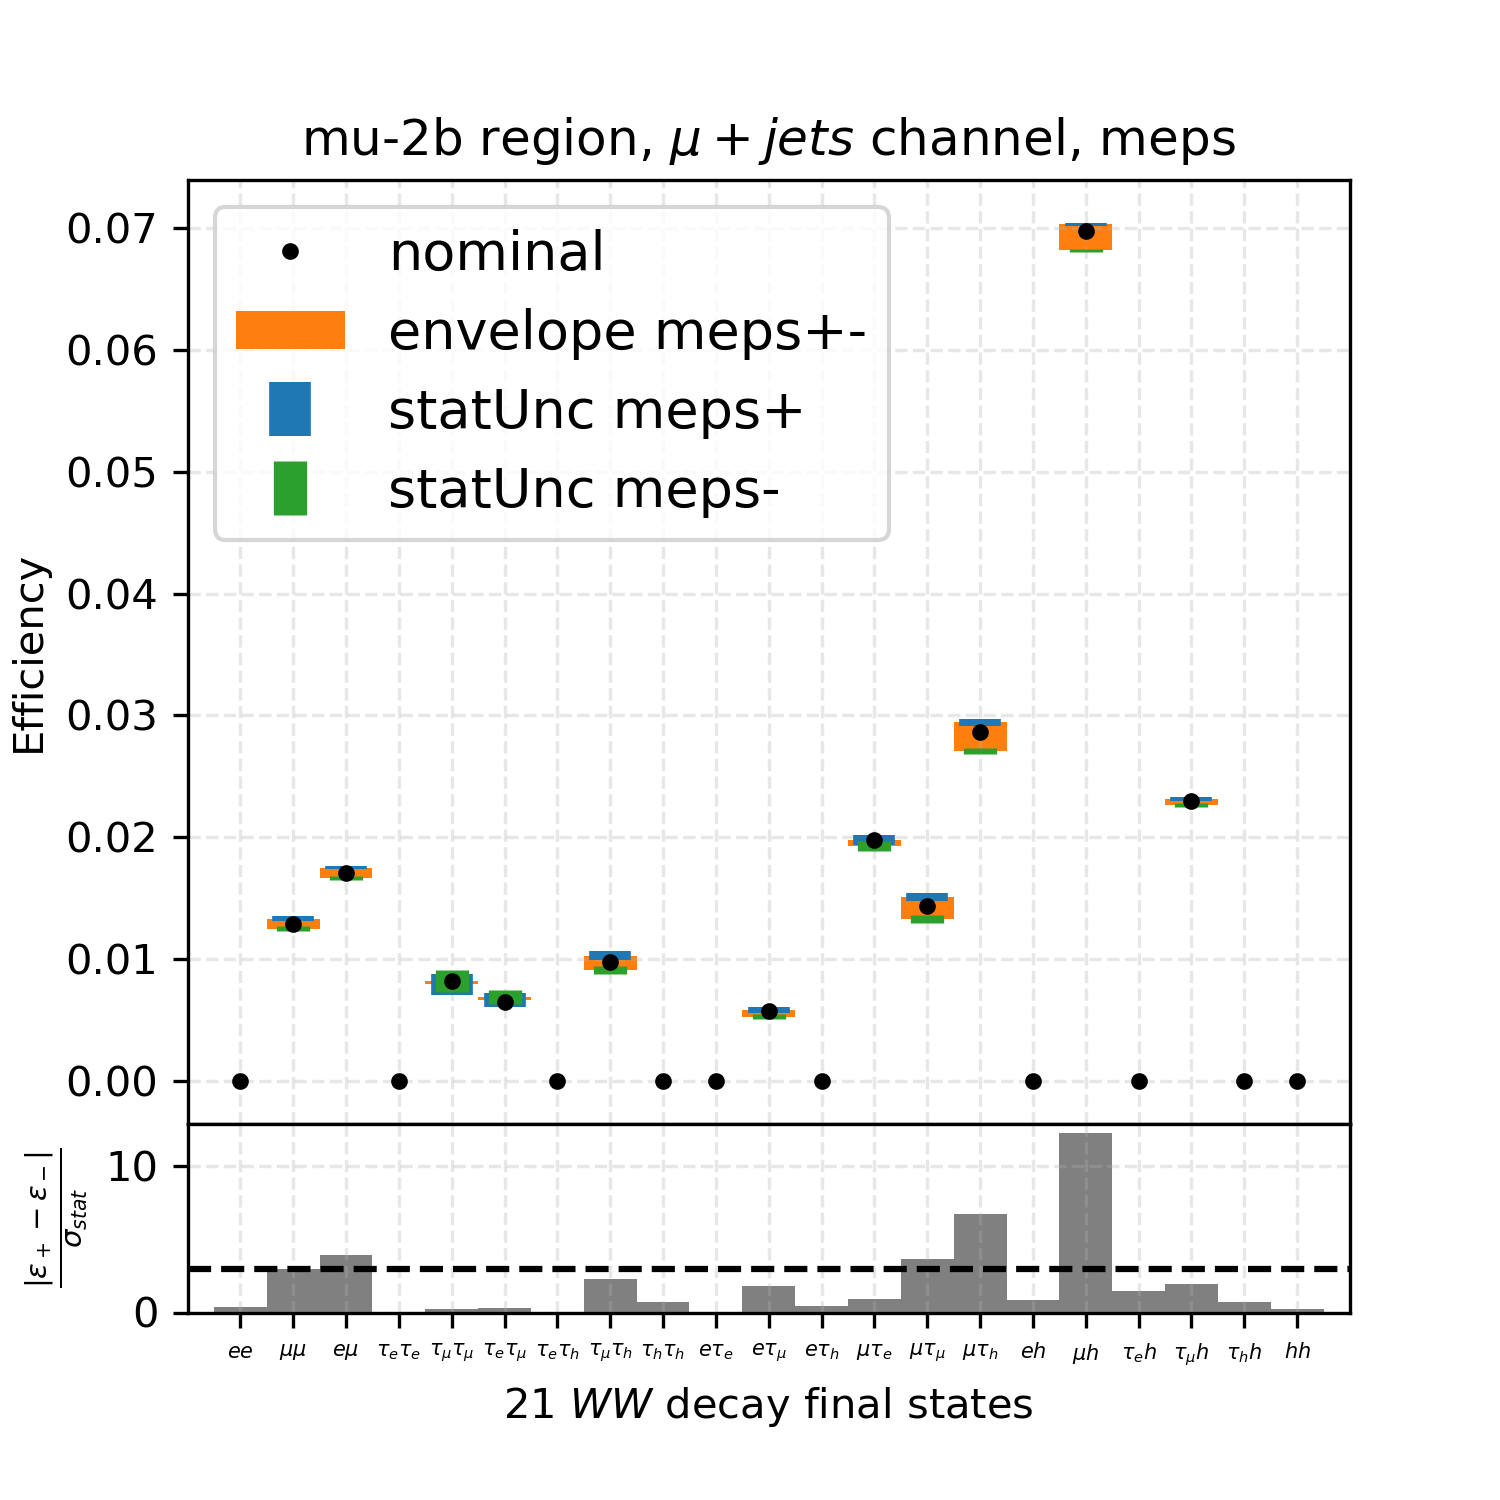
\includegraphics[width=0.24\textwidth]{chapters/Appendix/sectionTTSyst/figures/afterCorr/icata1_ch3_meps.png}
    
    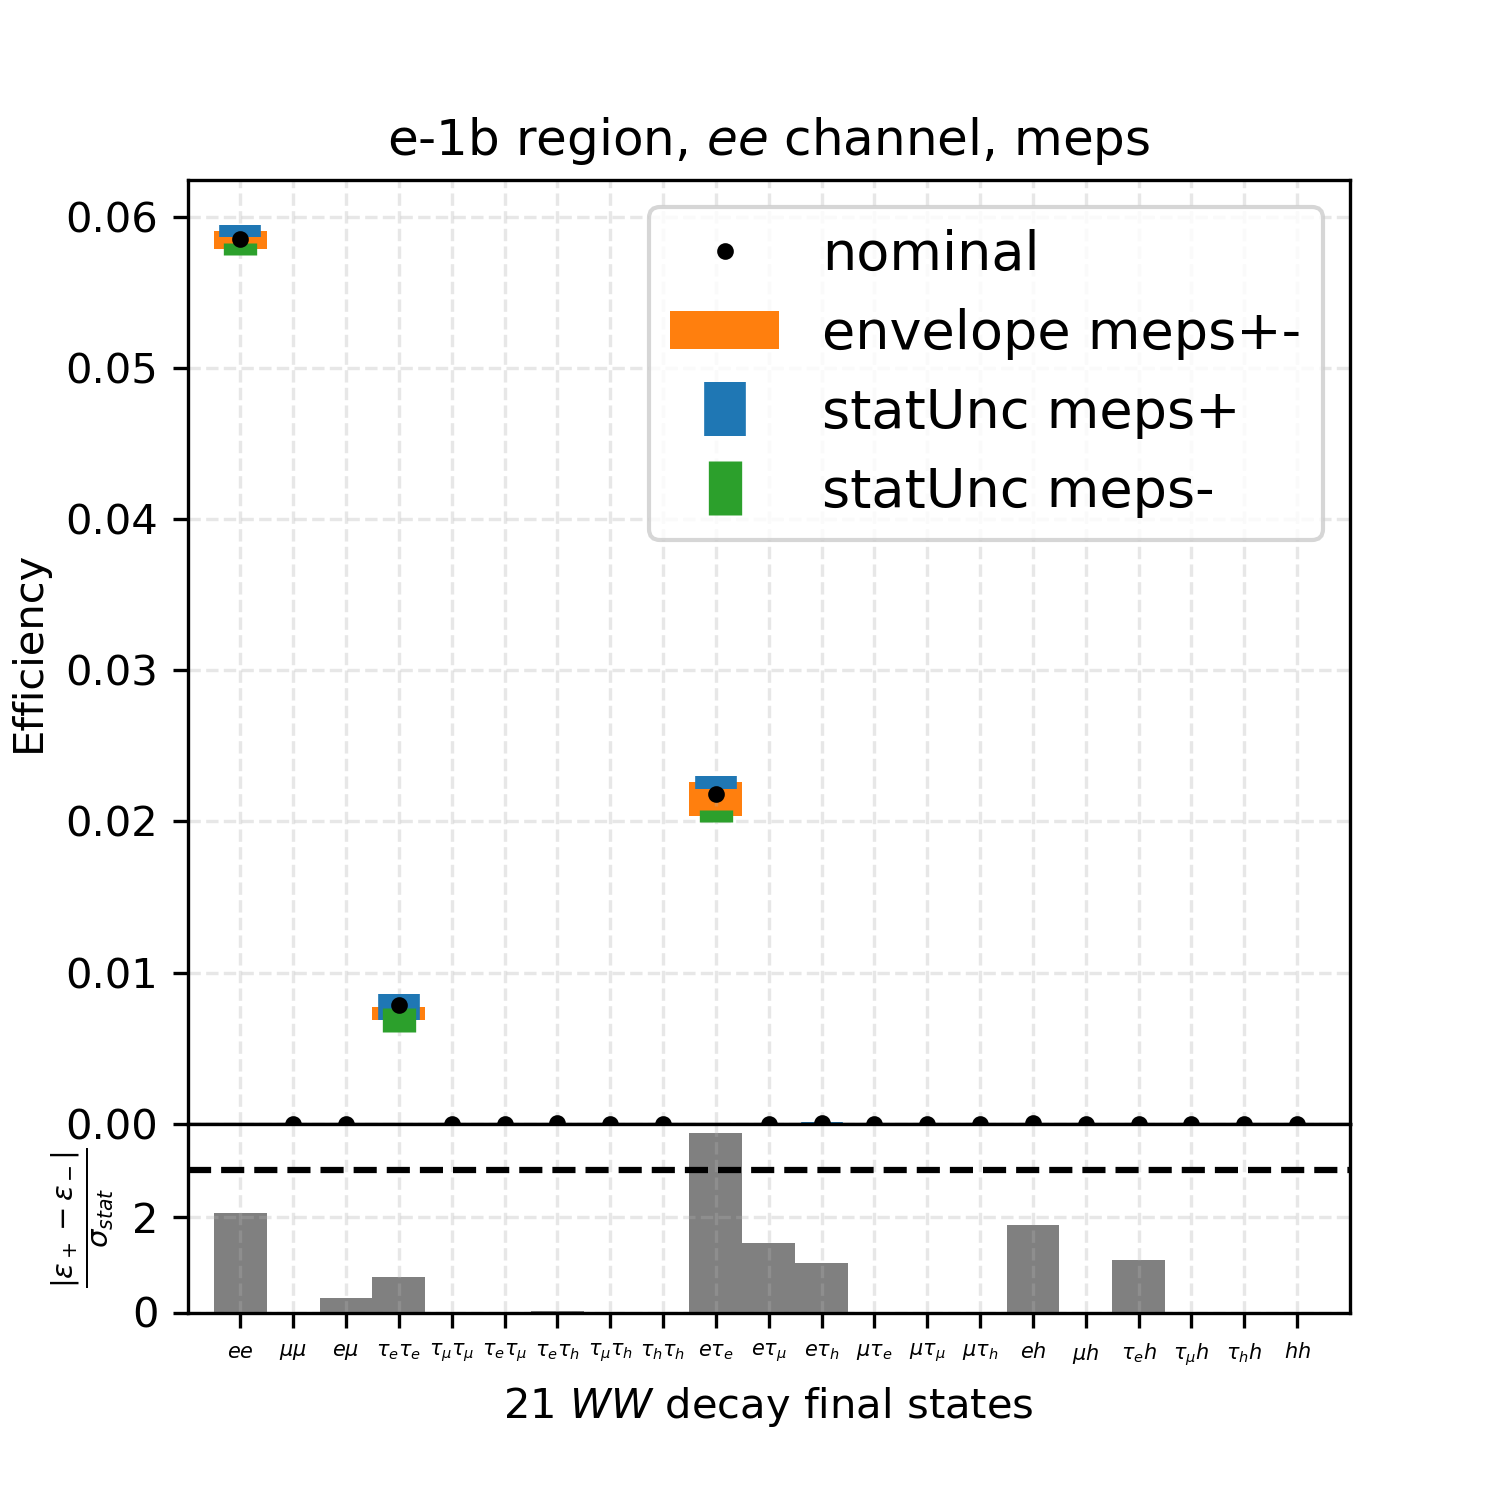
\includegraphics[width=0.24\textwidth]{chapters/Appendix/sectionTTSyst/figures/afterCorr/icata2_ch0_meps.png}
    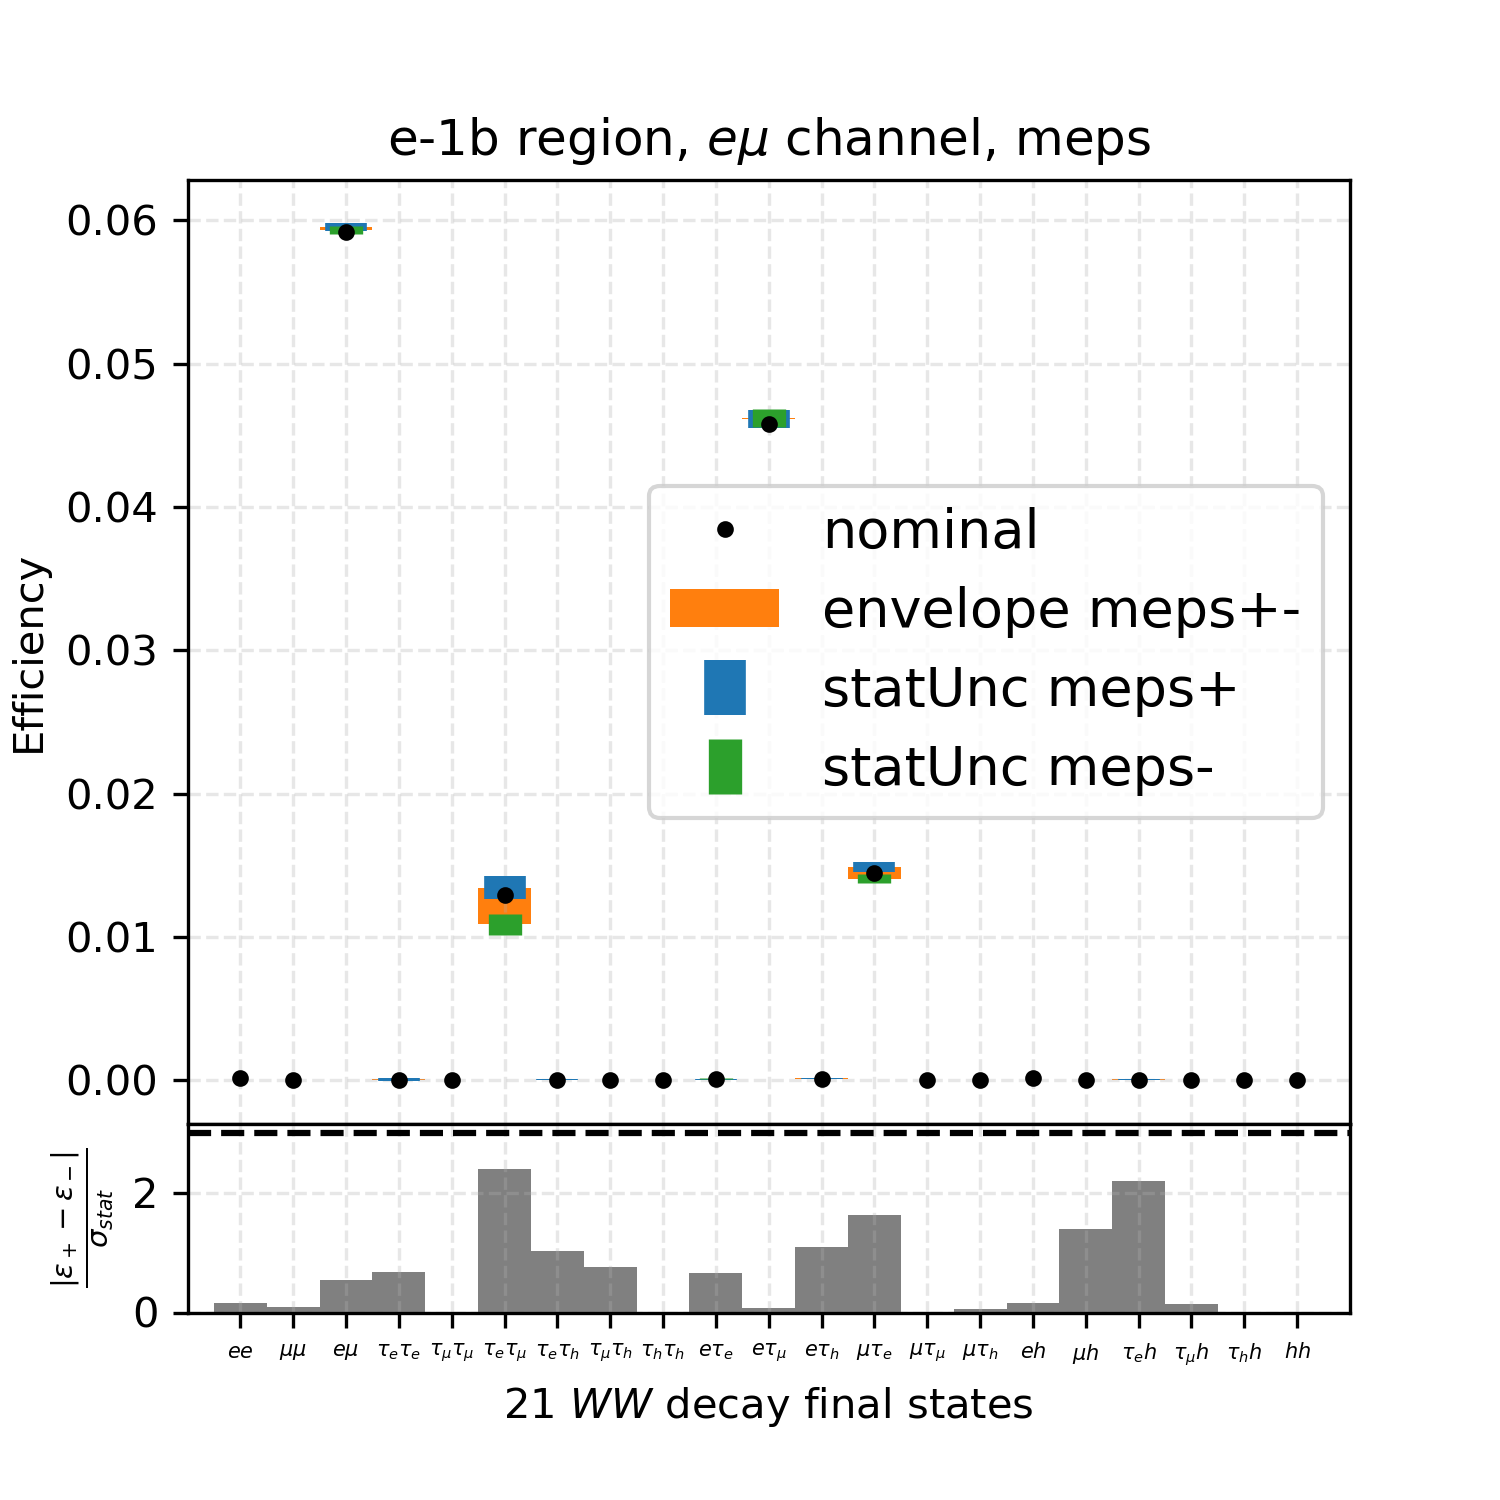
\includegraphics[width=0.24\textwidth]{chapters/Appendix/sectionTTSyst/figures/afterCorr/icata2_ch1_meps.png}
    \includegraphics[width=0.24\textwidth]{chapters/Appendix/sectionTTSyst/figures/afterCorr/icata2_ch2_meps.png}
    \includegraphics[width=0.24\textwidth]{chapters/Appendix/sectionTTSyst/figures/afterCorr/icata2_ch3_meps.png}

    \includegraphics[width=0.24\textwidth]{chapters/Appendix/sectionTTSyst/figures/afterCorr/icata3_ch0_meps.png}
    \includegraphics[width=0.24\textwidth]{chapters/Appendix/sectionTTSyst/figures/afterCorr/icata3_ch1_meps.png}
    \includegraphics[width=0.24\textwidth]{chapters/Appendix/sectionTTSyst/figures/afterCorr/icata3_ch2_meps.png}
    \includegraphics[width=0.24\textwidth]{chapters/Appendix/sectionTTSyst/figures/afterCorr/icata3_ch3_meps.png}
    
    \caption{Reweight $\tau_h$ and $j \to \tau_h$ efficiencies in the dedicated FSR, ISF, MEPS, UE ttbar samples}
    \label{fig:appendix:reweighttt:effAfterCorrFSR}
\end{figure}


\begin{figure}
    \centering
    \includegraphics[width=0.24\textwidth]{chapters/Appendix/sectionTTSyst/figures/afterCorr/icata0_ch0_ue.png}
    \includegraphics[width=0.24\textwidth]{chapters/Appendix/sectionTTSyst/figures/afterCorr/icata0_ch1_ue.png}
    \includegraphics[width=0.24\textwidth]{chapters/Appendix/sectionTTSyst/figures/afterCorr/icata0_ch2_ue.png}
    \includegraphics[width=0.24\textwidth]{chapters/Appendix/sectionTTSyst/figures/afterCorr/icata0_ch3_ue.png}

    \includegraphics[width=0.24\textwidth]{chapters/Appendix/sectionTTSyst/figures/afterCorr/icata1_ch0_ue.png}
    \includegraphics[width=0.24\textwidth]{chapters/Appendix/sectionTTSyst/figures/afterCorr/icata1_ch1_ue.png}
    \includegraphics[width=0.24\textwidth]{chapters/Appendix/sectionTTSyst/figures/afterCorr/icata1_ch2_ue.png}
    \includegraphics[width=0.24\textwidth]{chapters/Appendix/sectionTTSyst/figures/afterCorr/icata1_ch3_ue.png}
    
    \includegraphics[width=0.24\textwidth]{chapters/Appendix/sectionTTSyst/figures/afterCorr/icata2_ch0_ue.png}
    \includegraphics[width=0.24\textwidth]{chapters/Appendix/sectionTTSyst/figures/afterCorr/icata2_ch1_ue.png}
    \includegraphics[width=0.24\textwidth]{chapters/Appendix/sectionTTSyst/figures/afterCorr/icata2_ch2_ue.png}
    \includegraphics[width=0.24\textwidth]{chapters/Appendix/sectionTTSyst/figures/afterCorr/icata2_ch3_ue.png}

    \includegraphics[width=0.24\textwidth]{chapters/Appendix/sectionTTSyst/figures/afterCorr/icata3_ch0_ue.png}
    \includegraphics[width=0.24\textwidth]{chapters/Appendix/sectionTTSyst/figures/afterCorr/icata3_ch1_ue.png}
    \includegraphics[width=0.24\textwidth]{chapters/Appendix/sectionTTSyst/figures/afterCorr/icata3_ch2_ue.png}
    \includegraphics[width=0.24\textwidth]{chapters/Appendix/sectionTTSyst/figures/afterCorr/icata3_ch3_ue.png}
    
    \caption{Reweight $\tau_h$ and $j \to \tau_h$ efficiencies in the dedicated FSR, ISF, MEPS, UE ttbar samples}
    \label{fig:appendix:reweighttt:effAfterCorrFSR}
\end{figure}


\FloatBarrier
